% Improving Precipitation Phase Classification in Mountain Hydrology:
% A Machine Learning Framework Using Citizen Science and Gridded
% Meteorological Data
%
% Draft manuscript -- targeting AMS Artificial Intelligence for the
% Earth Systems (AIES). Uses the official AMS class ametsocv6.1.cls and
% bib style ametsocV6.bst 

% ======================================================================
% Submission/draft mode above (one column, 1.5 spacing, numbered lines).
% For a personal two-column, journal-style preview ONLY, use:
%   \documentclass[twocol]{ametsocV6.1}
% Always submit to AMS with \documentclass{ametsocV6.1}.

% \documentclass{ametsocV6.1} % uncomment for submission-ready format (figures pushed to end)
\documentclass[twocol]{ametsocV6.1} % uncomment to read personal review

% NOTE: ametsocv6.1.cls and the AMS bib style ametsocV6.bst ship with the
% official AMS LaTeX package (and the AMS Overleaf template). Place both
% files alongside this manuscript, or compile on Overleaf, to build the
% PDF -- they are not part of a standard TeX Live installation.

% Limit math alphabets to avoid "too many math alphabets" with newtxmath.
% \newcommand{\hmmax}{0}
% \newcommand{\bmmax}{0}

% ametsocv6.1.cls already loads: graphicx, amsmath, amsfonts, amssymb,
% bm, mathptmx, newtxtext, newtxmath, epstopdf, helvet, fancyhdr, natbib,
% url, xcolor, indentfirst, multicol, ifthen, rotating, appendix,
% setspace, lineno. Do NOT reload these. (Do not use subcaption or
% subfigure -- AMS disallows them; combine multi-panel figures into a
% single file instead.)
% Tables use the AMS-native \topline/\midline/\botline rules (no booktabs).

\graphicspath{{figures/}}

\newcommand{\degC}[1]{\ensuremath{#1\,^{\circ}\mathrm{C}}}
% --- TODO helper: red inline flags for unverified/missing content ---
\newcommand{\todo}[1]{\textcolor{red}{\textbf{[TODO: #1]}}}

%% ---------------------------------------------------------------------
%% Front matter. In the AMS class, \title, \authors, \affiliation, and
%% \abstract all precede \begin{document}.
%% ---------------------------------------------------------------------
\title{Improving Precipitation Phase Classification in Mountain
Hydrology: A Machine Learning Framework Using Citizen Science and
Gridded Meteorological Data}

% A more claim-orientied version, but doesn't start with ideal key words:
% \title{A Machine Learning Framework Based on Citizen Science and
% Gridded Meteorological Data Improves Precipitation Phase Classification in Mountain
% Hydrology}

\authors{Emma Golub,\aff{a}\correspondingauthor{Emma Golub,
emmaa.golub@gmail.com}
Nayoung Hur,\aff{a}
Meghan Collins,\aff{b}
and the Mountain Rain or Snow Citizen Scientists\aff{c}}

\affiliation{%
\aff{a}{Lynker, Louisville, CO}\\
\aff{b}{Desert Research Institute, Reno, NV}\\
\aff{c}{Mountain Rain or Snow project, \todo{coordinating institution}}}

\abstract{
  % TODO: one last past through, avoid repetition
Precipitation phase partitioning is a leading source of uncertainty in
mountain hydrology, where rain--snow misclassification degrades
streamflow forecasting and water-resource management. Conventional
methods that rely on sparse station networks and near-surface thermodynamic
thresholds are limited near freezing, where rain and snow distributions
overlap. We explore whether citizen-science observations and gridded
data can better predict phase there. Our framework
assimilates crowdsourced phase reports from the Mountain Rain or Snow
(MRoS) network with station meteorology and satellite-derived
probability of liquid precipitation, interpolates every source to an
hourly 1-km grid, and trains a calibrated machine learning model 
on held-out MRoS labels across California's Sierra Nevada and 
Colorado's Rocky Mountains from October 2022 to May 2026. 
Because mixed precipitation is difficult to classify as a distinct
phase, we instead compare observer-reported mixed events against the
model's own region of uncertainty, which flags where mixed phase is
likely. 
We benchmark against nine standard partitioning methods and quantify
significance with a paired cluster bootstrap. Test AUROC was 0.965 in
both domains (95\% CI 0.957--0.972 in California; 0.942--0.982 in
Colorado). Against the best benchmark, the model gained 11.1 percentage
points of accuracy in California (9.0--13.4) and 16.5 points near
freezing (12.2--21.1). Colorado's gains were smaller on accuracy (3.6
points, 0.2--6.9) but clearer on macro F1 (0.096, 0.042--0.152).
Ablations that retrain with inputs withheld trace these gains to the
assimilated predictors, above all the crowdsourced surfaces.
}

\begin{document}

\maketitle

%% ---------------------------------------------------------------------
%% Significance Statement (AMS: 120 words maximum). 
%% ---------------------------------------------------------------------
\statement
Predicting whether mountain precipitation falls as rain or snow is
essential for water-supply and flood forecasting. However, the process is challenging
and prone to errors near freezing temperatures, where sparse weather stations and simple
temperature-based partitioning methods struggle to correctly classify precipitation phase. 
We show that combining crowdsourced phase reports from volunteer observers 
with station, satellite, and terrain data on a common 1-km grid substantially 
improves rain--snow prediction across California and Colorado, especially near freezing.

% ======================================================================
\section{Introduction}
\label{sec:intro}

% Paragraph 1 -- Why phase matters: mountain hydrology and its forecast chain
% TODO: improve flow of this paragraph. snowpack --> streamflow timing --> melt vs runoff (seems a little back-forth)
Determining whether cold-season precipitation falls as rain or snow is a 
critical yet challenging area of research in mountain hydrology. 
Seasonal mountain snowpack supplies water to more than one-sixth of
the global population \citep{barnett2005} and governs streamflow timing and
magnitude. In the western United States, 53\% of total runoff originates as
snowmelt, rising to roughly 70\% in mountainous terrain
\citep{li2017snowrunoff}. Precipitation phase largely determines how that water is delivered. 
Snow accumulates through the winter and is released gradually during melt, whereas
rain runs off within hours, so a single storm can either recharge water supply
or trigger flooding depending on its phase. An error in phase classification
propagates quickly downstream, leading to inaccurate snowpack estimates, runoff timing,
flood magnitude estimation, and weather forecasts issued to mountain communities
and backcountry users \citep{harpold2017rain, jennings2019sensitivity}.
Morevoer, warming temperatures have been responsible in shifting cold-season
precipitation from snow to rain and increasing rain-on-snow flood risk across
western North America \citep{musselman2018}, both of which contribute to higher
uncertainty in water supply planning and hazards forecasting.

% Paragraph 2a -- Why it is hard: observational limits and mixed phase
Phase remains difficult to classify accurately, especially near freezing.
Precipitation gauges located in mountainous terrain are geographically sparse relative 
to the heterogeneous conditions they are intended to record. 
Few stations report phase at all, and those that do often sit where cold-air pooling, 
wind exposure, and steep elevation gradients decouple recorded estimates from true 
conditions in their surroundings \citep{lundquist2008rain, minder2011, wayand2016}. 
Precipitation phase also resists a clean definition: near freezing, 
hydrometeors may arrive as graupel, ice pellets, freezing rain, or wet mixtures that 
share a range of surface air temperatures (Section~\ref{sec:mix}). 
This known physical ambiguity has made classifying mixed precipitation separately
from rain or snow a predictive challenge and 
significant source of error.

% Paragraph 2b -- Why it is hard: methods and the predictor ceiling
Conventional phase partitioning models struggle to accurately predict phase. 
Most land surface, hydrologic, and snow models partition rain from snow with a single
near-surface air-temperature threshold or a smooth transition around one
\citep{ding2014, dai2008}. This approach measurably alters simulated
accumulation and melt \citep{jennings2019sensitivity} without translating to regions
where transitional phase temperatures can vary by more than \degC{4} \citep{jennings2018spatial}. 
Wet-bulb temperature supplements phase classification by capturing 
the cooling of hydrometeors falling through unsaturated air
\citep{harder2013, sims2015, wang2019}, but no surface measurement resolves
melting and refreezing aloft, so errors concentrate near freezing
\citep{feiccabrino2015}. Increasing model complexity does not necessarily fix the issue either; 
\citet{jennings2025} found that fine-tuning machine learning models
marginally improves phase predictions that rely on simple partitioning 
rules and near-surface meteorology.

% Paragraph 3 -- The observational gap and crowdsourcing
% TODO: fix this paragraph
Addressing this predictive accuracy ceiling requires exploring new model inputs. 
Ground-based phase reports at transition-zone elevations can supplement 
synoptic weather stations, which are sparse and typically biased toward
lower elevations and airports. Crowdsourcing helps fill atmospheric
observations where instruments are absent \citep{muller2015}, and the
Mountain Rain or Snow (MRoS) project explores this through collecting
timestamped, geolocated visual reports from citizen scientist volunteers across mountain
regions \citep{arienzo2021}. Such reports have helped in characterizing rain--snow
from mixed conditions and have been used in benchmarking phase partitioning methods 
\citep{jennings2023mros,jennings2025}. To our knowledge, their value as a 
predictor---assimilated alongside station and satellite data into a spatially continuous, 
probabilistic field---has yet to be explored.

% Paragraph 4 -- This study: research questions and contributions
This study explores how to overcome existing limitations in phase prediction. 
The following three research questions frame this work:
\begin{enumerate}
  % TODO: refine these questions
  \item Do assimilated predictors (i.e., interpolated
  crowdsourced phase observations, interpolated station meteorology, 
  and satellite-derived probability of liquid precipitation (pLP)) 
  improve rain--snow accuracy beyond what near-surface thermodynamics alone can supply?
  \item Does this data assimilation approach enhance predictive phase accuracy 
  near freezing where conventional threshold partititioning methods fail?
  \item Can mixed precipitation, which is usually discarded or
  forced into an ill-defined third class, exhibit meaningful signal in a model's
  region of predictive uncertainty?
\end{enumerate}

\noindent The framework we propose combines four complementary sources of data:
crowdsourced phase reports from MRoS, hourly station meteorology,
satellite pLP from GPM IMERG \citep{huffman2020imerg}, and topographical elevation. 
The combination of these data types makes up in strength for what each lacks on its own. 
Stations are typically accurate but provide sparse data points. Satellite products
capture a precipitating column but with coarse resolution. Crowdsourced observations
are similarly sparse and can be biased to one storm but can report phase that actually 
reached the ground where stations are absent. 
The station meteorology and crowdsourced observations are interpolated into their own surfaces,
which are then assimilated with resampled IMERG pLP and elevation onto a common hourly 1-km grid.

We train an XGBoost classifier \citep{chen2016} on held-out MRoS phase labels and
evaluate it in two climatologically distinct ranges, California's Sierra
Nevada and Colorado's Rocky Mountains, which differ in precipitation pattern, terrain, 
and observer density. After bootstrapping with clustered resampling to quantify significance
and produce confidence intervals for each prediction, we benchmark against the standard partitioning methods 
surveyed by \citet{jennings2025}.

% ======================================================================
\section{Study domains and period}
\label{sec:domains}

Two mountain domains are processed independently through an identical
pipeline: the California Sierra Nevada / Lake Tahoe region (UTM Zone 11N,
EPSG:26911) and the Colorado Rocky Mountains (UTM Zone 13N, EPSG:32613).
Each area of interest is bounded by a polygon over mountain terrain, the
study period spans 1 October 2022 to 1 May 2026 (excluding June, July, and August 
as the summer non-observation season), and all datasets are harmonized to a common 1-km
analysis grid whose coordinates and elevations derive from a digital
elevation model (DEM). The domains contrast usefully
(Figure~\ref{fig:domain}): California has much wider covariation of air
temperature with elevation, atmospheric-river-driven storms, and a
comparatively balanced observation mix, whereas Colorado's continental
snow climate is strongly snow-dominant with sparser rain.

\begin{figure*}[tp]
  \centering
  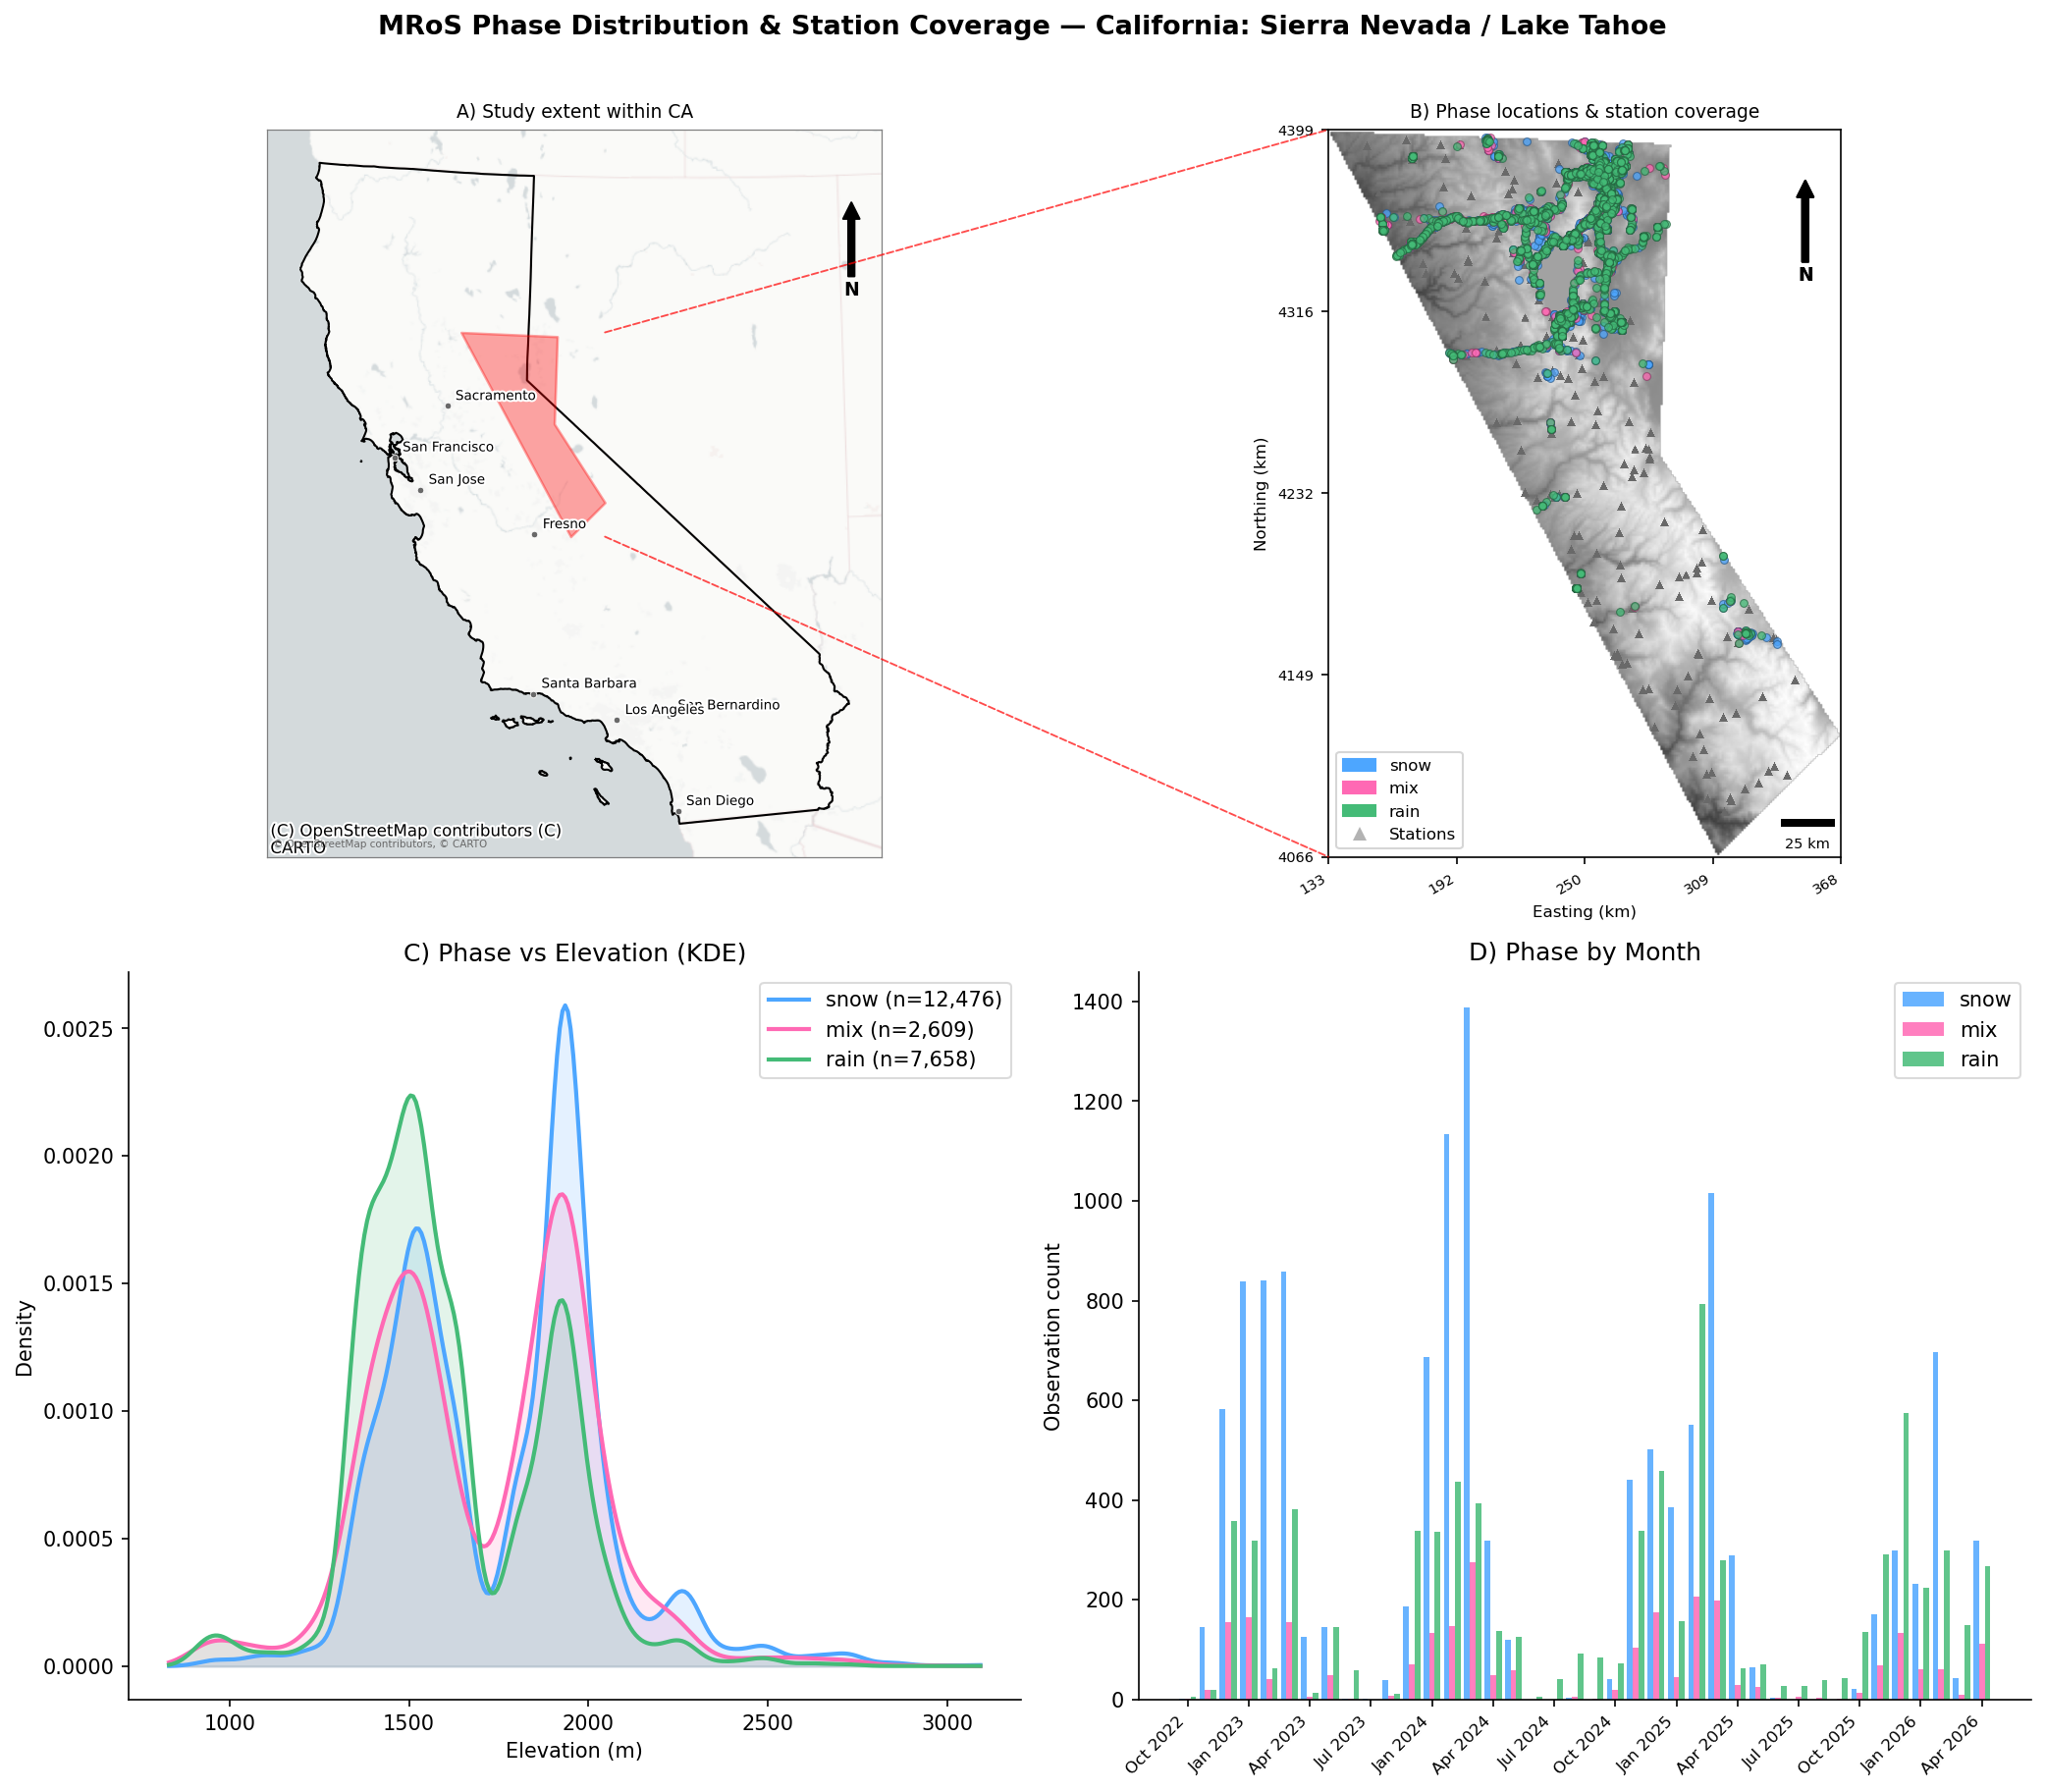
\includegraphics[width=\textwidth,height=0.42\textheight,keepaspectratio]{CA/mros_phase_diagnostics_combined_CA.png}\\[6pt]
  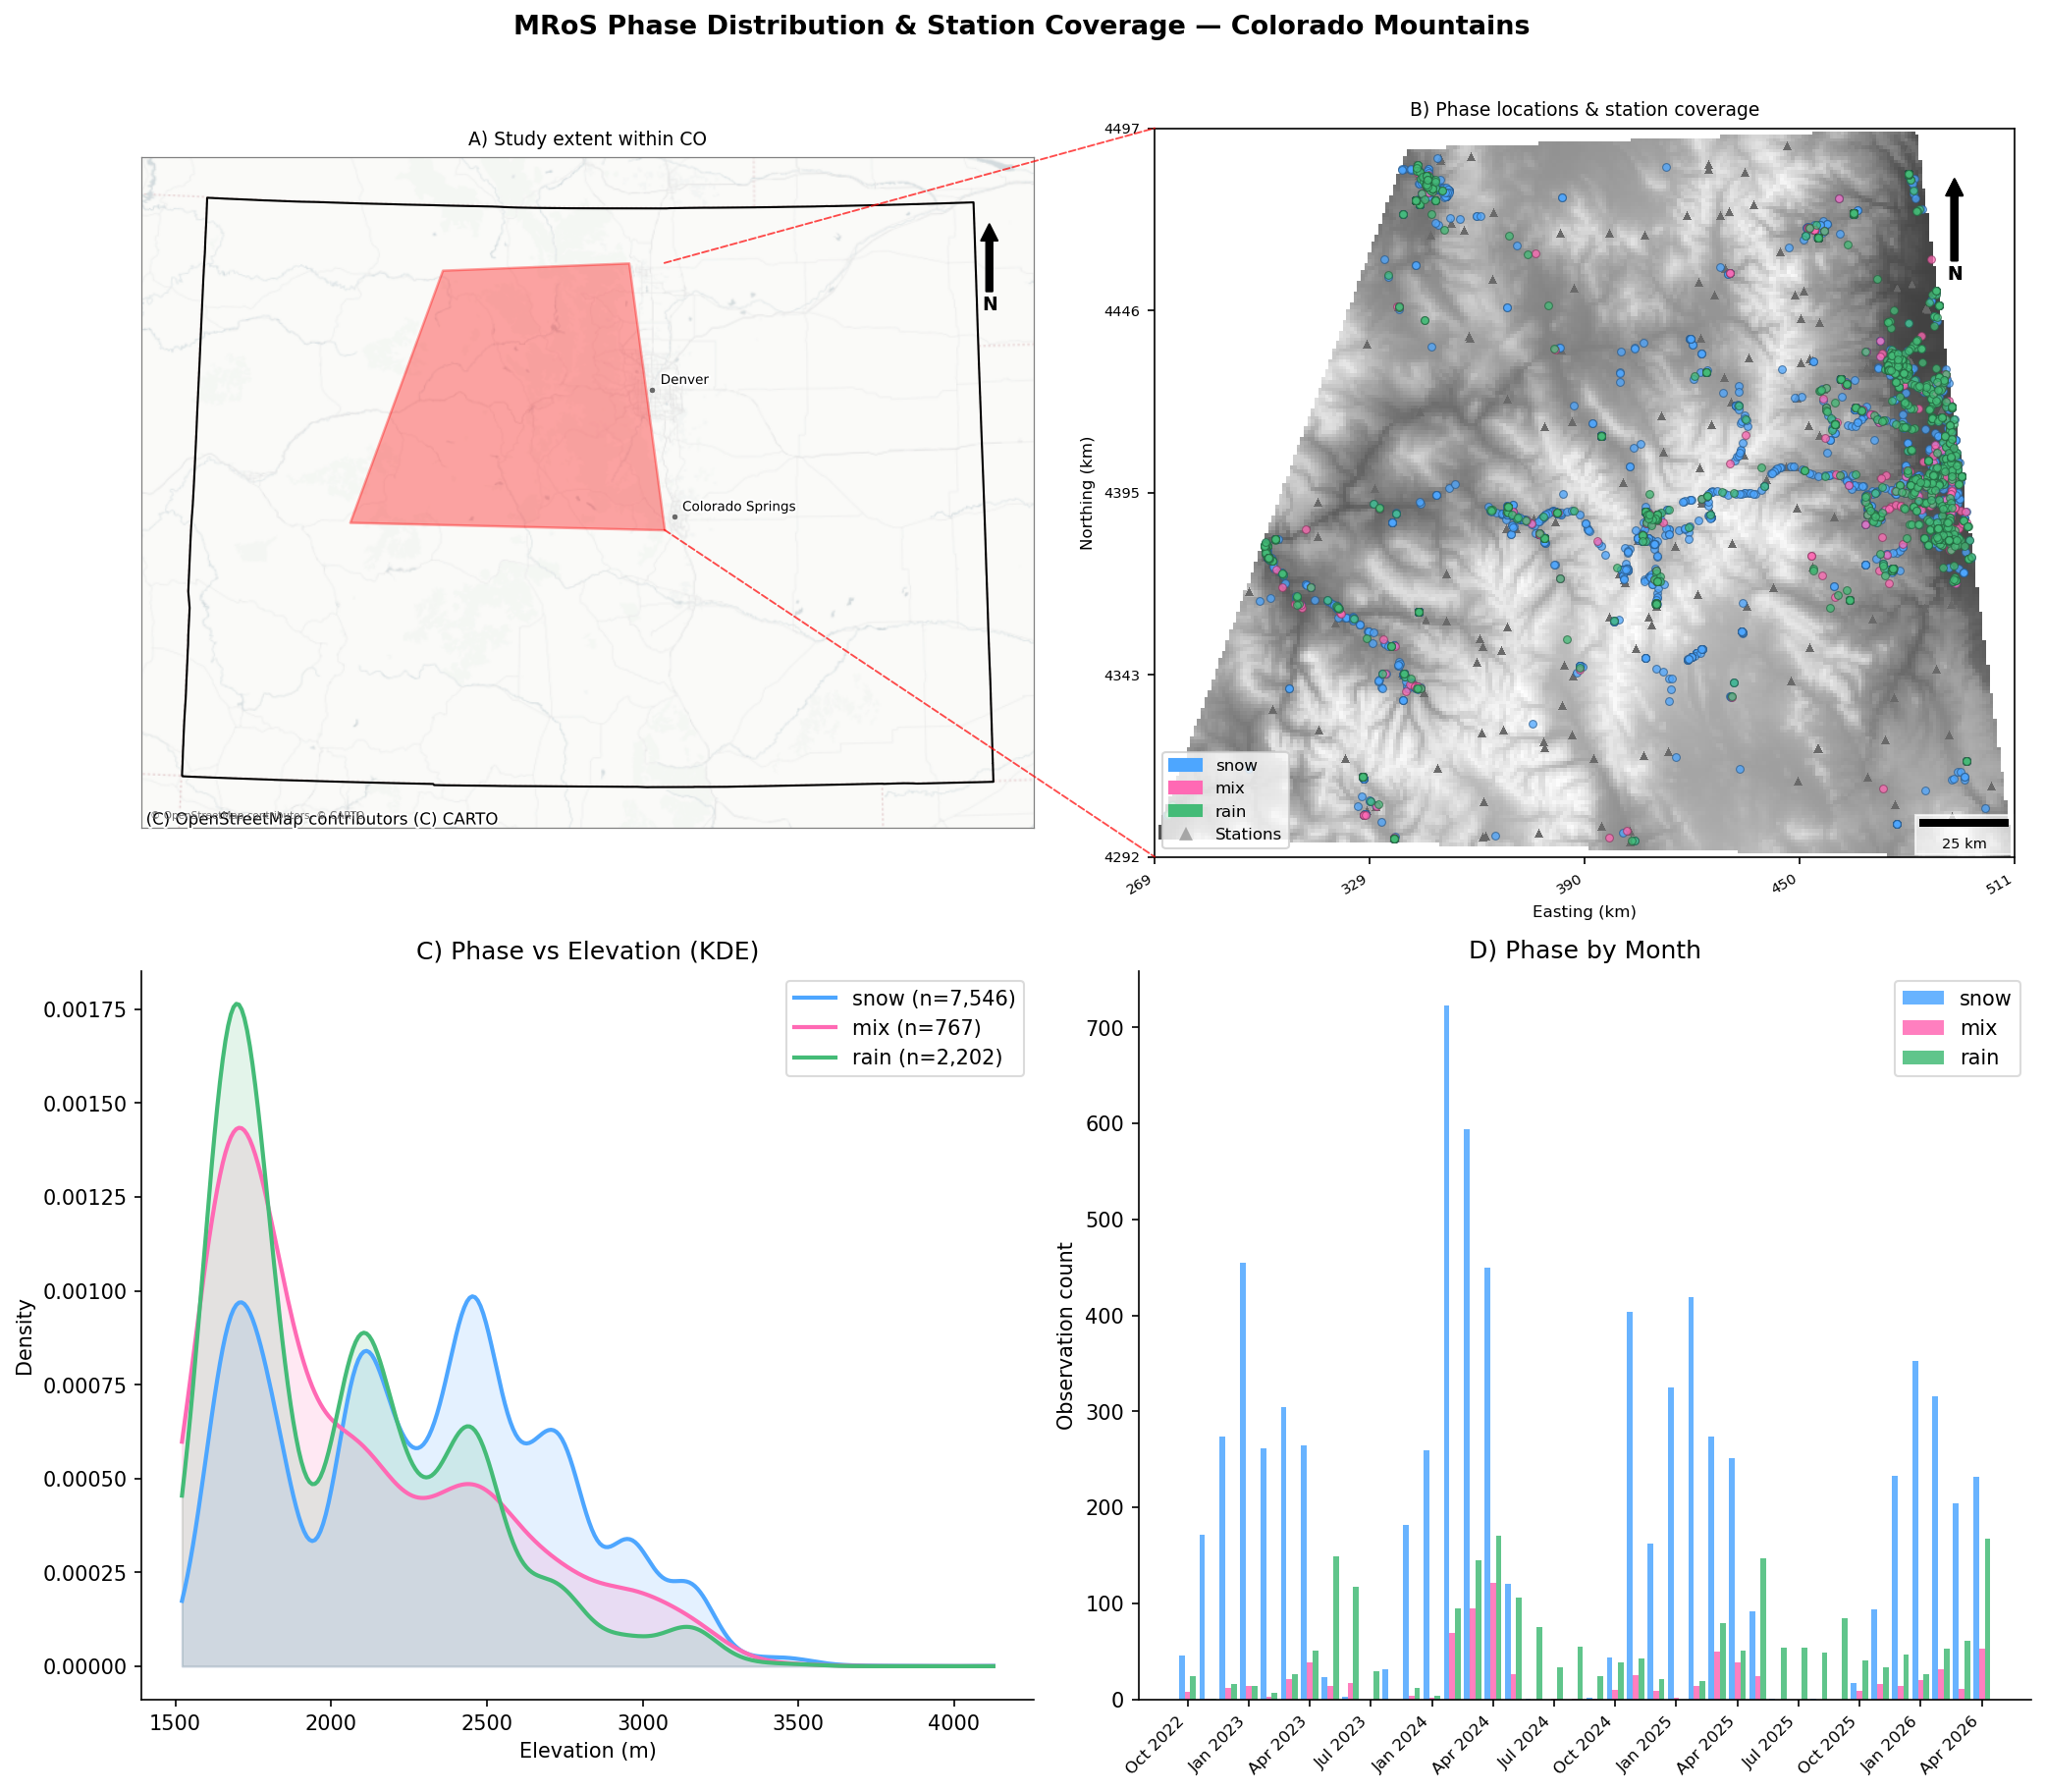
\includegraphics[width=\textwidth,height=0.42\textheight,keepaspectratio]{CO/mros_phase_diagnostics_combined_CO.png}
  \caption{Study domains and observation distribution for (a, top) California's
  Sierra Nevada and Lake Tahoe and (b, bottom) Colorado's Rocky
  Mountains. Within each block: (A) study extent (red) within the state;
  (B) MRoS reports over shaded relief, colored by reported phase, with
  assimilated surface stations as grey triangles; (C) kernel density of
  report elevation by phase; and (D) monthly report counts by phase.
  Panel C is density-normalized within each phase, so the curves compare
  shape rather than volume; phase totals appear in the legend
  (California 12{,}476 snow, 2{,}609 mix, 7{,}658 rain; Colorado 7{,}546
  snow, 767 mix, 2{,}202 rain).
  %
  California's reports are bimodal in elevation, rain-dominated near
  1500~m and snow-dominated near 1950~m, whereas Colorado's peak near
  1700~m with secondary snow modes above; this is the
  elevation--temperature covariation invoked later to explain
  California's non-monotonic skill structure. Two sampling caveats apply
  throughout: reports cluster along road corridors and near population
  centers, so panel B reflects observer access as much as precipitation
  frequency, and panel D counts are participation-driven with near-total
  summer gaps, so they are not storm climatology.}
  \label{fig:domain}
\end{figure*}

% ======================================================================
\section{Data}
\label{sec:data}

% TODO: reconcile language tense

\subsection{Crowdsourced phase observations}
MRoS citizen scientists submit timestamped, geolocated reports of
precipitation phase (rain, snow, or mixed) during storm events
\citep{arienzo2021}. Volunteers who have opted into storm text alerts,
issued when forecast surface temperatures fall in the rain--snow
uncertainty range of roughly $-2$ to \degC{10}, open a browser-based app
during precipitation and record what phase is currently falling; the
device supplies geolocation and timestamp automatically. The protocol
operationalizes the phase definitions of Section~\ref{sec:intro}:
observers report what is falling rather than what has accumulated,
classify graupel as snow and freezing rain as rain, exclude hail and true
sleet, and reserve the mixed label for genuinely ambiguous or rapidly
transitioning precipitation. That last instruction matters, because it
makes the mixed label an explicit report of observer uncertainty rather
than a claim about a distinct hydrometeor type. Neither temperature nor
intensity is entered by the observer, so each record reduces to a
geotagged, timestamped phase label.

Each submission is processed with the \texttt{rainOrSnowTools} package
\citep{rainorsnowtools}, which tags it with USGS 3DEP elevation and with
modeled surface meteorology from stations within a one-degree radius
(requiring at least five stations) after standardized range and
consistency checks. Quality assurance follows the procedures established
for the network \citep{arienzo2021, jennings2023mros}: only real-time
reports are retained, since ancillary fields are matched to each report's
exact time and location, and observations lacking nearby station support
or failing physical plausibility checks are removed. After this, the
rain--snow observation set comprises 15{,}337 observations in
California (10{,}735 train / 2{,}301 validation / 2{,}301 test; 64\% snow)
and 3{,}492 in Colorado (2{,}444 / 524 / 524; 82\% snow).
Observer-reported mixed events constitute a further 12.2\% of California
test observations (320 of 2{,}621) and 10.9\% of Colorado's (64 of 588);
they are held aside from binary training and used for uncertainty-band
evaluation (Section~\ref{sec:mix}).

% TODO: describe here how MRoS labels are interpolated into three surfaces?

\subsection{Station meteorology}
Hourly surface observations are collected from four public networks
(HADS, LCD, WCC, and MADIS) via the \texttt{rainOrSnowTools} access
layer \citep{rainorsnowtools}. The retained variables are air
temperature, dewpoint, and relative humidity, from which wet-bulb
temperature is derived during assimilation (Section~\ref{sec:assim}).
These stations provide the thermodynamic environment that is
interpolated to the analysis grid.

\subsection{Satellite probability of liquid precipitation}
Half-hourly GPM IMERG probability-of-liquid-precipitation (pLP) fields
\citep{huffman2020imerg} are retrieved from NASA GES DISC via OPeNDAP,
subset server-side to each domain, and merged across the 48
half-hourly timesteps into daily gridded tables. pLP is an independent,
satellite-derived estimate of precipitation phase (only rain or snow) from passive
microwave and infrared retrievals and later becomes a key model
predictor: it carries information about the precipitating column that 
near-surface measurements cannot typically supply.

\subsection{Reanalysis climate fields (explored, not used)}
\label{sec:reanalysis}
We explored daily PRISM rasters \citep{daly2008} as a spatially
complete backdrop to the sparse station network, resampling five
variables from 800~m to the 1-km grid. PRISM regridded cleanly in space,
however its daily resolution is too coarse for an hourly phase product. 
Expanding it to hourly required imposing a diurnal temperature
curve, and that synthetic sub-daily structure did not improve validation
skill over the station-interpolated fields while risking bias near
freezing. We therefore excluded it.
Coarser global reanalyses (ERA5, MERRA-2) were similarly rejected
because their 30--50-km resolutions cannot resolve the kilometer-scale
elevational gradients that control phase here.

\subsection{Terrain}
Raw 10-m DEMs from the USGS 3DEP / National Map are clipped to each
domain, reprojected to the regional UTM CRS, and resampled to 1 km by
average pooling. The resulting DEM defines the analysis grid and supplies
the elevation field used for lapse-rate detrending, kriging drift, and as
a model predictor.

\begin{table*}[tp]
  \centering
  \caption{Model predictors and their sources. All fields are
  harmonized to the hourly 1-km analysis grid.}
  \label{tab:predictors}
  \begin{tabular}{lll}
    \topline
    Predictor & Source & Native resolution \\
    \midline
    Air temperature & HADS/LCD/WCC/MADIS stations, interpolated & point, hourly \\
    Dewpoint temperature & Stations, interpolated & point, hourly \\
    Wet-bulb temperature & Derived \citep{stull2011} & --- \\
    Elevation & USGS 3DEP DEM & 10 m \\
    IMERG pLP & GPM IMERG \citep{huffman2020imerg} & $0.1^{\circ}$, half-hourly \\
    MRoS $p_{\mathrm{snow}}, p_{\mathrm{mix}}, p_{\mathrm{rain}}$ &
    LOOCV-interpolated MRoS reports & point, hourly \\
    \botline
  \end{tabular}
\end{table*}

\noindent Table~\ref{tab:predictors} lists the final predictor set,
which comprises eight fields once the three MRoS surfaces are counted
separately (discussed in (Section~\ref{sec:interp})). 
Relative humidity is interpolated and used to derive dewpoint and 
wet-bulb temperature, but it is not itself supplied to the model
(Section~\ref{sec:reanalysis}).
% TODO: describe why RH isn't used? or referenced appropriately in sec?

% ======================================================================
\section{Methods}
\label{sec:methods}

The methodology divides into two pipelines that are run identically per domain.
A data-preparation pipeline (Sections~\ref{sec:assim}--\ref{sec:interp})
fuses station meteorology, external gridded products, and MRoS reports,
then interpolates them onto the common analysis grid, producing gridded
predictor fields and leakage-safe MRoS phase-probability predictors. A
modeling pipeline (Sections~\ref{sec:ml}--\ref{sec:uq}) trains and
calibrates the binary classifier, derives the mixed-phase uncertainty
band, and evaluates the result through ablation, benchmarking, and a
clustered bootstrap. Figure~\ref{fig:architecture} summarizes the full
data-assimilation and modeling architecture.

\begin{figure*}[tp]
  \centering
  \includegraphics[width=0.9\textwidth]{architecture.png}
  \caption{Data-assimilation and machine-learning architecture. (a) Inputs:
  crowdsourced MRoS phase reports, surface station networks (HADS, LCD,
  WCC, MADIS), GPM IMERG probability of liquid precipitation (pLP), and
  the USGS 3DEP elevation model resampled to the \mbox{1-km} grid. (b)
  Station observations and MRoS reports are kriged to that grid per
  domain and timestamp, producing the predictor stack sampled at each
  report location. (c) An XGBoost snow-versus-rain classifier is fit
  separately per domain on eight predictors, its scores are
  beta-calibrated, and the wet-bulb-conditioned band of
  Equation~\ref{eq:band} is applied. (d) Output is snow, rain, or an
  uncertainty flag.
  %
  Two design choices govern how the rest of the paper should be read.
  The classifier is binary throughout, and the uncertainty flag is a
  post-hoc rule applied to the calibrated score, not a third trained
  class. And mixed events are withheld from training entirely, serving
  only as held-out ground truth for evaluating band placement, which is
  why mix capture is a diagnostic rather than a classification score.}
  \label{fig:architecture}
\end{figure*}

\subsection{Data assimilation and quality control}
\label{sec:assim}
An assimilation stage cleans the station record, derives consistent
meteorology, and harmonizes every source to the DEM grid before
interpolation. Missing thermodynamic variables are reconstructed from
physical relationships: saturation vapor pressure follows
Magnus--Tetens, dewpoint and relative humidity are interchanged to fill
whichever is missing, and wet-bulb temperature, the most physically
informative single predictor of phase, is estimated with Stull's formula
\citep{stull2011}, refined by an iterative psychrometric solution and
constrained between dewpoint and air temperature. Where a station
reports air temperature without co-located humidity, dewpoint and
relative humidity are gap-filled at the station using
lapse-rate-adjusted inverse-distance weighting (IDW) from neighboring
stations, following the \texttt{model\_meteo} procedure of
\texttt{rainOrSnowTools} \citep{rainorsnowtools}.

Station observations then pass through quality control: duplicates are
dropped, hard physical cutoffs remove impossible readings, a per-station
interquartile-range filter removes outliers, spike and stuck-sensor
detection nulls implausible runs, and cross-variable checks reconcile
temperature with humidity. Survivors are aggregated to one record per
station per hour. A dynamic lapse rate is estimated at each timestep from
the station temperature--elevation relationship, letting the vertical
structure vary hour to hour, and DEM elevation is appended to every point
dataset so all sources share an elevation reference. IMERG is brought to
the hourly 1-km grid by bilinear resampling, and all retained fields are
synchronized on a common UTC axis and written to hourly NetCDF stacks.

\subsection{Spatial interpolation}
\label{sec:interp}
All point observations are interpolated to the 1-km analysis grid by
kriging, the best linear unbiased predictor for a spatial field
\citep{cressie1993, goovaerts1997}. Kriging estimates an unsampled
location as $\hat{Z}(\mathbf{s}_0) = \sum_{i=1}^{n}
\lambda_i\,Z(\mathbf{s}_i)$, with weights $\lambda_i$ that minimize
estimation variance subject to unbiasedness. Those weights are set by
the spatial dependence structure, summarized by the empirical
semivariogram over observation pairs separated by lag $\mathbf{h}$,
\begin{equation}
  \hat{\gamma}(\mathbf{h}) = \frac{1}{2\,|N(\mathbf{h})|}
  \sum_{(i,j)\in N(\mathbf{h})} \left[Z(\mathbf{s}_i) - Z(\mathbf{s}_j)\right]^2 ,
  \label{eq:variogram}
\end{equation}
to which a spherical model was fitted operationally. Because hourly
observations are sparse, we pool the empirical semivariogram across time
before fitting, which stabilizes the covariance estimate during thinly
observed hours.

Each variable is kriged in the form matched to its physical nature. Air and
dewpoint temperature carry a strong elevation trend, so they are
detrended against station elevation with the hourly lapse rate,
interpolated by ordinary kriging on the residuals, and retrended with DEM
elevations, a regression-kriging that preserves physical vertical
structure \citep{hengl2007}. Relative humidity is interpolated by
universal kriging with DEM elevation as an external drift term
\citep{wackernagel2003}, so its terrain dependence enters the trend
directly.

Precipitation phase is nominal, so encoding snow, mix, or rain ordinally and
interpolating would impose artificial arithmetic (i.e., mix would represent a 
meaningless average of snow and rain). We therefore convert phase to one-hot indicators, krige each
class independently by indicator kriging \citep{journel1983}, then clip
to non-negative values and renormalize so the three probabilities sum to
one, yielding hourly surfaces $p_{\mathrm{snow}}$, $p_{\mathrm{mix}}$,
$p_{\mathrm{rain}}$. Figure~\ref{fig:interpolations} shows the full set
at one storm timestamp per domain.

\paragraph{Leakage prevention.}
MRoS observations serve both as training labels and---through the
interpolated phase surfaces---as candidate predictors. Reading an
observation's predictor from a full-grid surface built with that same
observation would let the label leak into the feature. To break the
dependence we compute the MRoS phase predictors by pointwise spatial
leave-one-out cross-validation (LOOCV): each report is removed from its
hour, the remaining reports in that hour are re-kriged by indicator
kriging to the held-out location under the same minimum-neighbor
requirement, and the resulting triplet is clipped, renormalized, and
stored as the leakage-safe predictor. What remains is the phase implied
by other observers nearby, which is legitimate spatial context
available at inference time rather than the target label itself.
Full-grid surfaces built from all observations are retained separately
for mapping and gridded prediction, never as training features. This
mirrors the leave-one-out logic used for unbiased local estimates in
geostatistical cross-validation \citep{goovaerts1997}.

\begin{figure*}[tp]
  \centering
  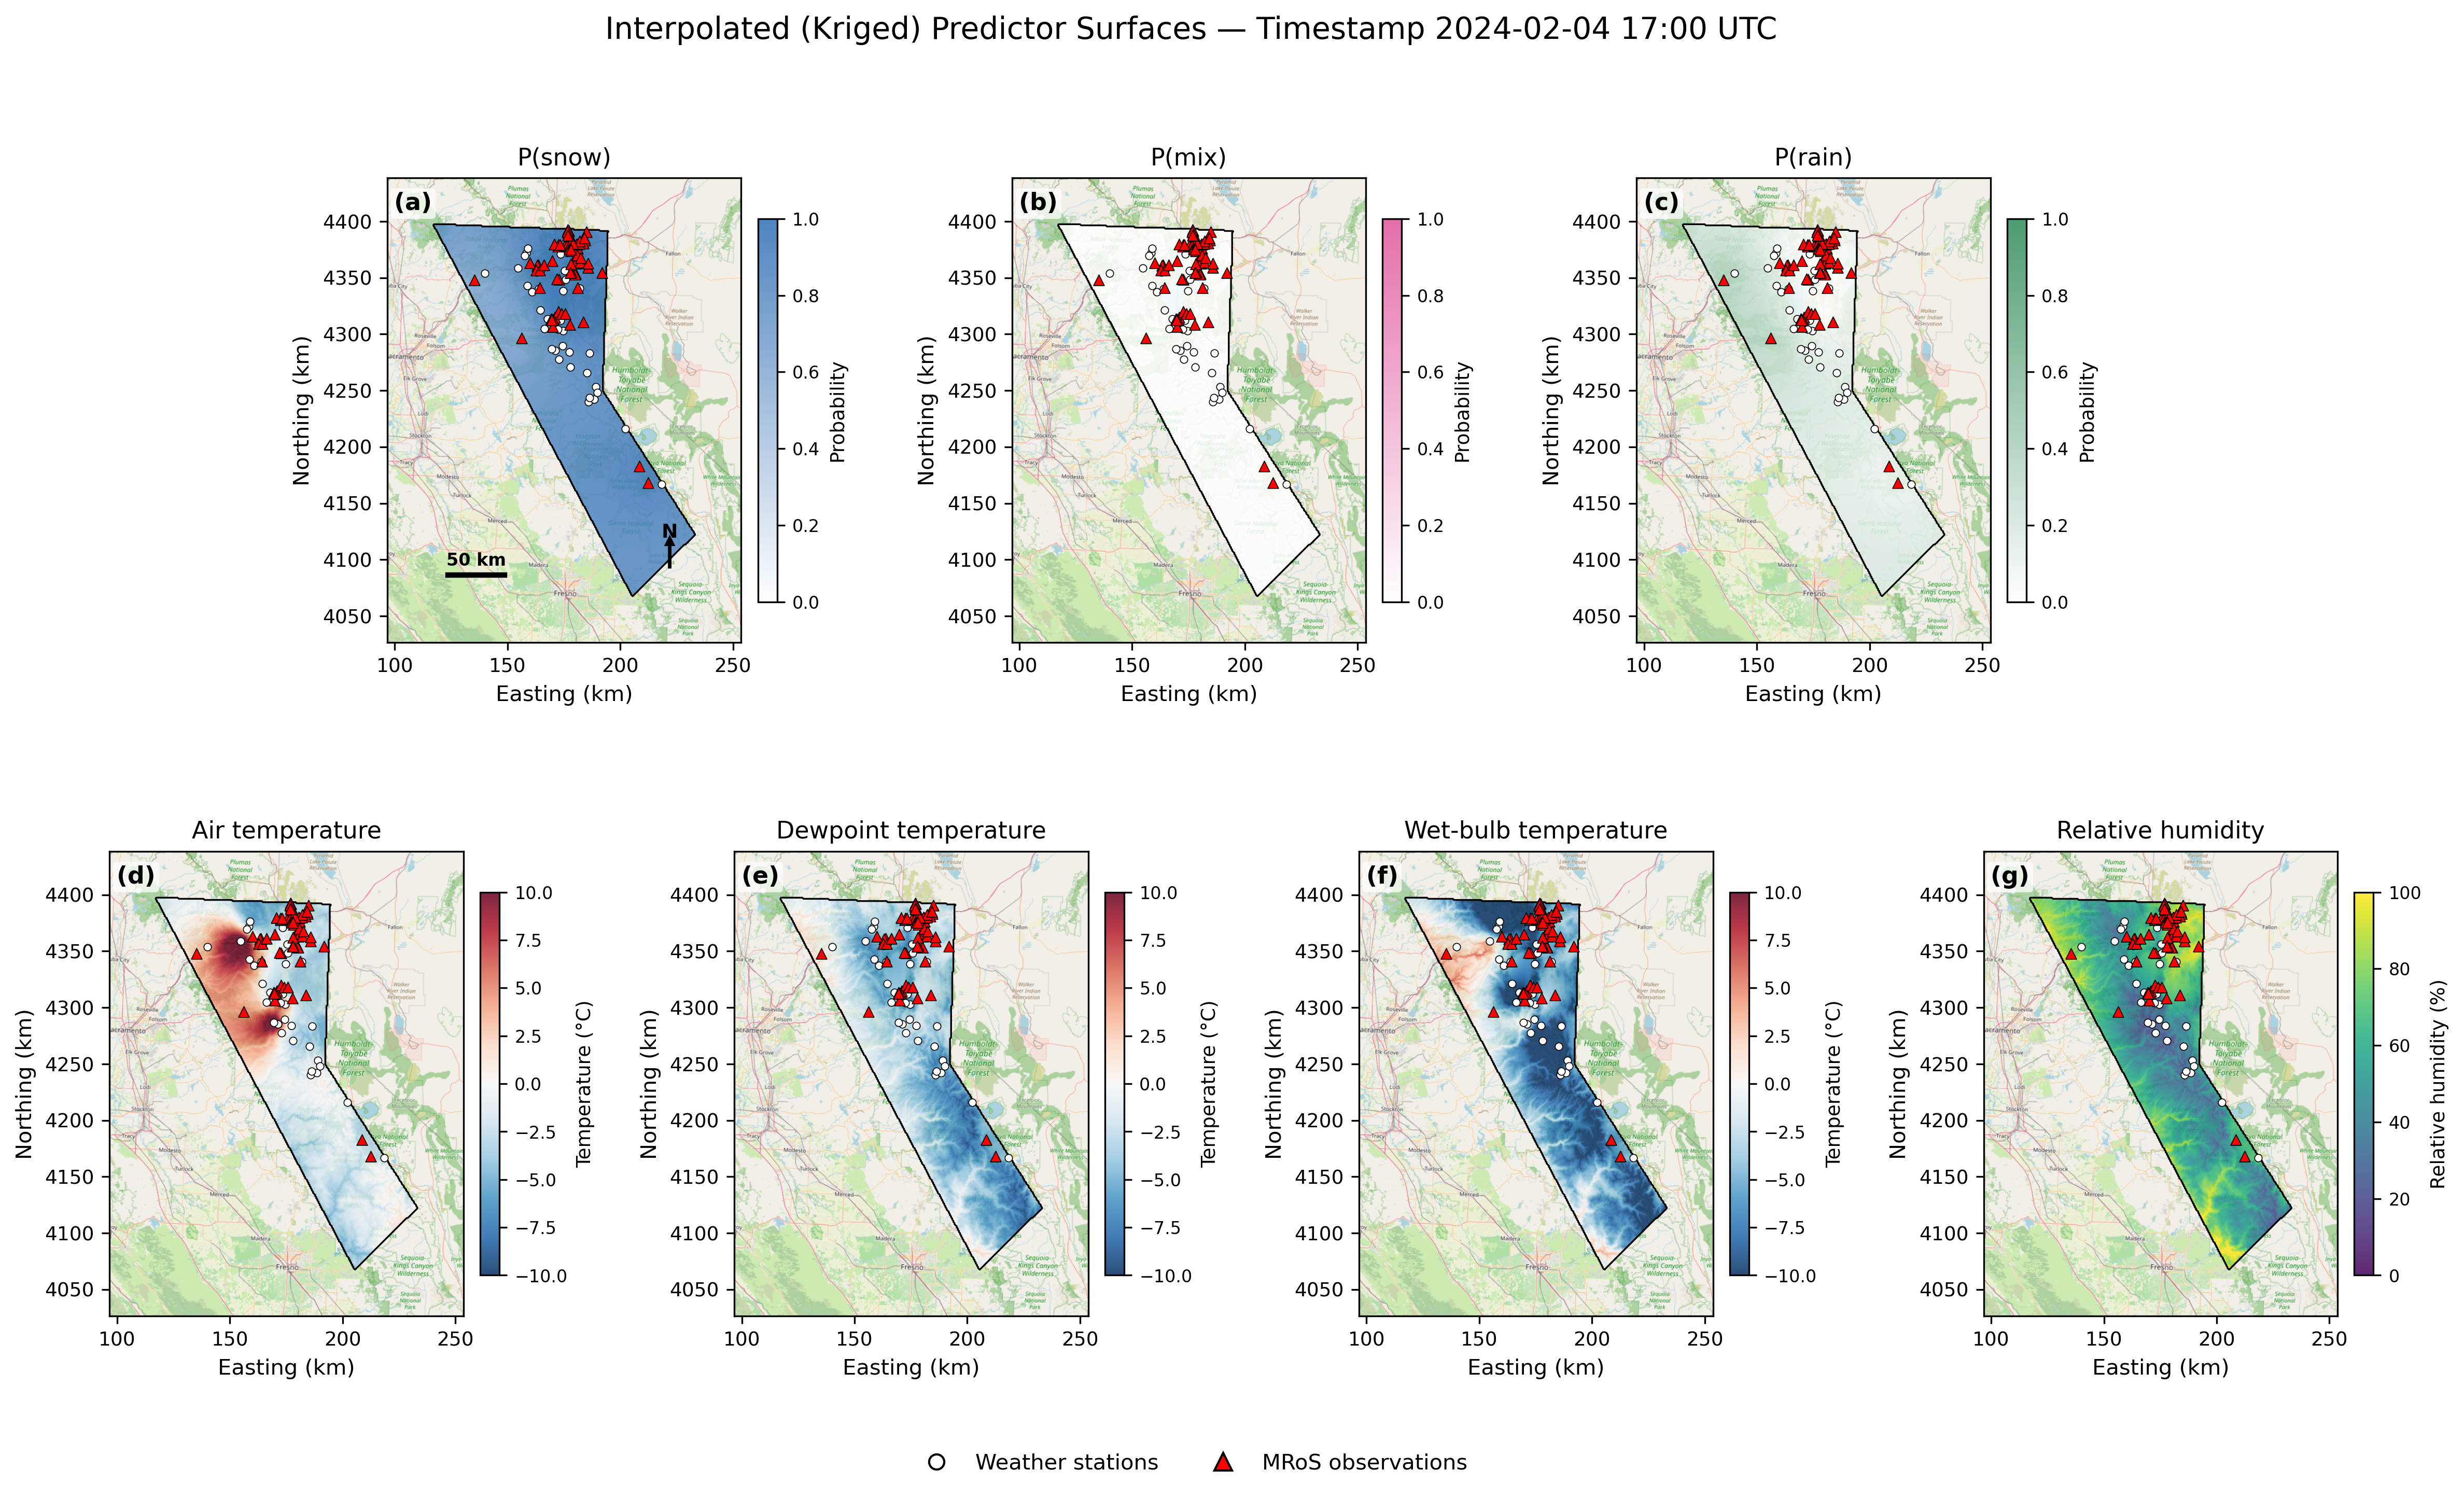
\includegraphics[width=0.95\textwidth]{CA/quicklook_20240204T1700Z.png}\\[2pt]
  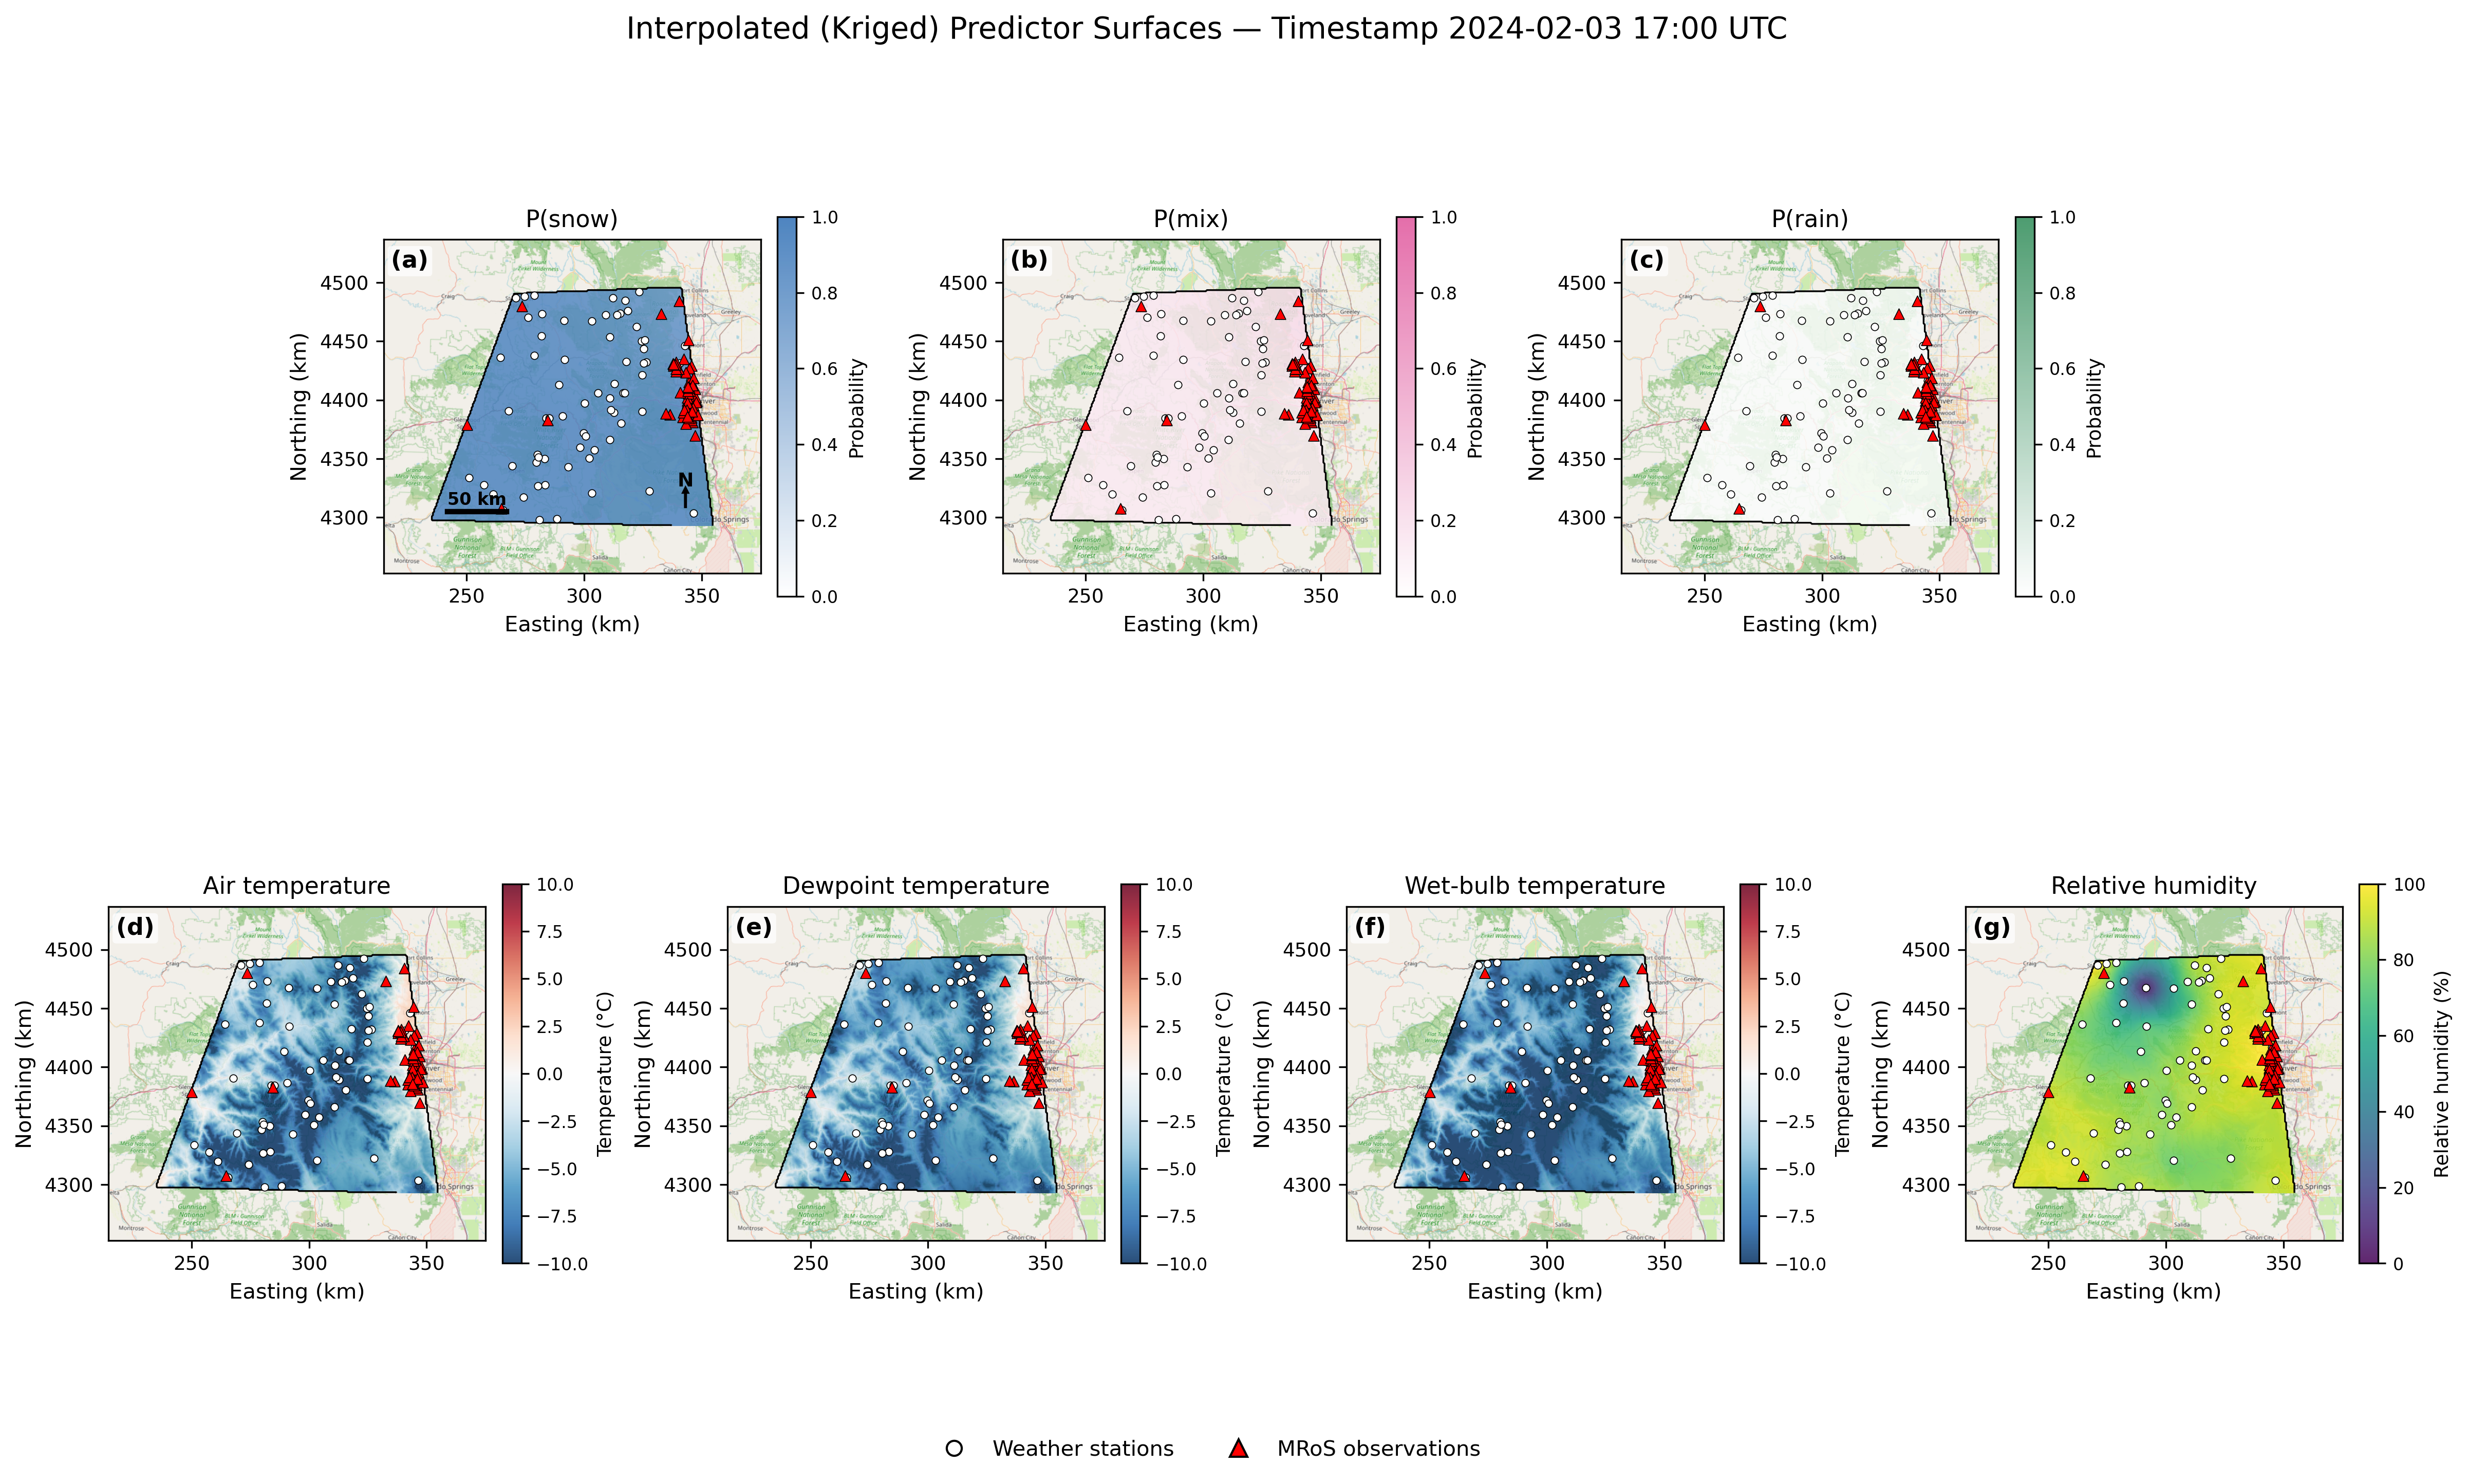
\includegraphics[width=0.95\textwidth]{CO/quicklook_20240203T1700Z.png}
  \caption{Kriged predictor surfaces on the \mbox{1-km} analysis grid for (a, top)
  California at 2024-02-04 17:00 UTC and (b, bottom) Colorado at
  2024-02-03 17:00 UTC, two independent storm timestamps. Within each
  block, panels (a)--(c) are the kriged MRoS phase probabilities and
  panels (d)--(g) are kriged air, dewpoint and wet-bulb temperature and
  relative humidity. Open circles mark contributing stations, red
  triangles MRoS reports at that timestamp.
  %
  Three features matter for the model. The fields are smooth by
  construction, so they represent mesoscale structure rather than local
  microclimate and residual sub-grid variability is absorbed into the
  uncertainty band rather than resolved. Predictor skill degrades away
  from the observation clusters, most visibly in the sparsely
  instrumented southern Sierra. And these are the full-data surfaces;
  the model predictor is the leave-one-out version, so the value a
  training report sees at its own location excludes that report and is
  necessarily noisier than shown here.}
  \label{fig:interpolations}
\end{figure*}


\subsection{Machine learning model}
\label{sec:ml}
We frame phase prediction as binary classification and train an
XGBoost model \citep{chen2016} with a logistic objective on rain--snow
observations only. We refer to the resulting eight-predictor
configuration as "MRoS-XGB" throughout for simpler mention. 
% TODO: fix the above sentence.
The output is the probability of snow,
with $p(\mathrm{rain}) = 1 - p(\mathrm{snow})$. Gridded predictors are
sampled at each MRoS observation location from the hourly NetCDF
stacks, giving eight predictors: air, dewpoint, and wet-bulb
temperature, elevation, IMERG pLP, and the three leakage-safe LOOCV
MRoS phase probabilities. Data are split 70/15/15 into
train/validation/test, stratified on observed phase class with a fixed
random seed, and early stopping is applied on the validation subset (up
to 2{,}000 rounds, patience 50; selected iterations 323 in CA and 513
in CO).

Two discarded alternatives motivate this structure. A multiclass
version trained snow/mix/rain directly and was abandoned because mixed
precipitation does not form a separable cluster in feature space
(Section~\ref{sec:mix}). A second version kept binary training but used
spatially blocked splits with Platt-scaled calibration, and was
abandoned because blocking left calibration sets too small to fit
stably across thermodynamic regimes. The randomized stratified split
adopted here instead preserves the distribution of meteorological
states across subsets, matching the evaluation design of
\citet{jennings2025}, and defers the residual spatial correlation to
the inference stage (Section~\ref{sec:uq}). Its known cost is that
observations from the same storm may appear in both train and test, so
test performance may be mildly optimistic relative to a novel season.

\paragraph{Class imbalance.}
Both training sets skew toward snow (64\% in California, 82\% in
Colorado), and the skew is not simply a matter of counts. The MRoS
network favors higher-elevation, snowier sites, and those sites are also
colder, drier, and carry higher LOOCV snow probabilities, so the class
imbalance is entangled with the feature space. Left uncorrected it
produces a model that favors snow, surfacing as snow recall exceeding
rain recall and doing most damage near the transition, where a missed
rain call is the error that matters for runoff timing. The standard
remedy, frequency-inverse weighting, balances the effective counts but
does not target the recall asymmetry itself, and because the geographic
and thermodynamic skews compound, it can over- or under-correct. We
therefore tune XGBoost's \texttt{scale\_pos\_weight} against the
quantity of interest; a probe model is trained across a grid of
candidate weights and the value minimizing the absolute snow--rain
recall gap on the validation set is selected (0.50 for California, 0.15
for the more snow-dominant Colorado). Both fall below one, downweighting
the majority snow class, and the resulting recalls balance to within
0.03 and 0.06 respectively (Section~\ref{sec:skill-results}). Because
class weighting shifts the raw score distribution, calibration follows
it rather than preceding it.

\paragraph{Probability calibration.}
\label{par:calibration}
A classifier can rank cases correctly while reporting probabilities that
do not verify. Gradient-boosted trees are particularly prone to this,
since each boosting round drives training loss down by pushing scores
toward 0 and 1, and the resulting overconfidence is amplified under class
imbalance and by the weighting above. That matters here because
downstream applications need a $p(\mathrm{snow})$ that means what it
reports, and because the uncertainty envelope discussed further in Section~\ref{sec:mix}
is an interval in probability space whose placement is meaningful only if
the probabilities are.

We therefore fit a post-hoc map from raw score to calibrated probability.
Two features of the problem shape how. First, discrimination near
\degC{0} wet-bulb differs fundamentally from discrimination far from
freezing, because near freezing the thermodynamic signal is weak and true
probabilities compress toward 0.5 while away from freezing they approach
0 or 1. One map cannot serve both regimes, so we fit separate calibrators
for near-freezing ($|T_w| \le \degC{2}$, consistent with the
\citealt{sims2015} uncertainty range) and clear-phase, meaning
away-from-freezing, observations,
routing each by its wet-bulb temperature.

Second, the choice of calibrator matters more than usual for a
well-separated classifier. Isotonic regression, the conventional
non-parametric choice, failed diagnostically here: held-out scores fell
outside the range seen during fitting, and the out-of-range clipping
mapped 62\% of test predictions to exactly 0 or 1, inflating log loss
while leaving the Brier score untouched. That is the signature of a
calibrator reintroducing the overconfidence it was meant to remove. We
therefore adopt beta calibration \citep{kull2017}, which is parametric,
monotone, and defined on the open unit interval, so it cannot produce
degenerate outputs, and whose three parameters let the map be asymmetric
where the score distribution is. Calibrators are fitted on
final-booster scores over the pooled train and validation rain--snow
observations and applied forward to the untouched test set; mixed
observations are excluded entirely. Calibration adjusts probability
magnitudes only, leaving rank ordering and hard decisions unchanged.

\subsection{Handling mixed phase with an uncertainty envelope}
\label{sec:mix}
Because rain and snow are more physically defined than mix
(Section~\ref{sec:intro}), standard treatments tend to mishandle
that asymmetry. Discarding observer-reported mix, as most partitioning
studies do, throws away the observations closest to the very transition
the model is supposed to resolve. Training mix as a third class instead
presumes it is a well-defined category, which it is not: mixed labels are
only 11 to 12\% of the total, they overlap both pure snow--rain phases across the
same near-freezing temperatures rather than occupying a distinct region
of feature space, and observers can apply the label inconsistently. A trained
third class therefore learns mostly label noise while degrading the
rain--snow boundary, which is what our first multiclass iteration found
(Section~\ref{sec:ml}).

We take a third route: keep the supervised problem binary and treat mix
as a region of irreducible uncertainty in the model's own output.
Calibration settles what $p(\mathrm{snow})$ means, so the remaining
question is where the binary model stops being trustworthy. A fixed
threshold pair such as 0.30/0.70 is physically unjustified, because the
meaning of an intermediate score depends on thermodynamic context. Near
\degC{0} wet-bulb, where snow and rain routinely coexist in the same
column, $p(\mathrm{snow}) = 0.65$ is genuinely ambiguous; at
$T_w = \degC{-5}$ the same score would instead signal a real anomaly. We
therefore let the threshold width vary continuously with wet-bulb
temperature through a Gaussian half-band $h(T_w)$ applied post-hoc to the
calibrated probabilities:
\begin{equation}
  \begin{aligned}
    h(T_w) &= b + a\,\exp\!\left(-\frac{T_w^2}{2\sigma^2}\right),\\
    \text{rain threshold} &= 0.5 - h(T_w),\\
    \text{snow threshold} &= 0.5 + h(T_w),
  \end{aligned}
  \label{eq:band}
\end{equation}
The band is centered at $T_w = \degC{0}$ and decays as a Gaussian of
width $\sigma$, with $b$ setting the minimum half-width far from
freezing and $a$ the additional widening at \degC{0}
(Figure~\ref{fig:band}). Any observation whose calibrated
$p(\mathrm{snow})$ falls inside the band is flagged as uncertain rather
than assigned a phase. We call this an \emph{uncertainty envelope} to
emphasize that it does not predict a mixed class but delineates, in
probability space, the zone within which the binary model loses confident
discrimination and thus abstains from making a distinct call. 
Observer-reported mix events then serve as an independent
check on whether that zone lands where real mixed precipitation occurs.

Two metrics follow from this construction, defined in
Table~\ref{tab:metrics}: the \emph{flag rate}, a ground-truth independent 
property of model behavior, and the
\emph{mix-capture rate}, conditional on observer labels. They vary
independently, since a model can flag frequently and still miss real mix if
the envelope is centered wrongly, or abstain rarely and capture most of it
if the envelope is well placed. Comparing the two helps explore the functionality
of the model's uncertainty envelope.

The three band parameters are optimized on the validation set, which
for this purpose alone includes the observed mixed events. We optimize
a composite of mix capture and confident rain--snow accuracy, subject
to a minimum rain--snow coverage constraint, with $\sigma$ bounded to
physically reasonable transition-zone widths \citep{sims2015,
jennings2025}. The fitted parameters are identical in both domains
($b = 0.20$, $a = 0.15$, $\sigma = \degC{2.0}$), placing the thresholds
at $p < 0.15$ for rain and $p > 0.85$ for snow at \degC{0} wet-bulb and
relaxing them to $0.30$ and $0.70$ far from freezing.

\subsection{Evaluation framework}
\label{sec:eval-framework}
The framework is evaluated in three ways. A feature ablation
(Section~\ref{sec:ablation-methods}) retrains the model with inputs
withheld to establish which sources the skill depends on. A
benchmark comparison (Section~\ref{sec:bench-methods}) scores it
against operational partitioning methods, overall and near freezing. And
the uncertainty envelope is assessed against observer-reported mixed
events (Section~\ref{sec:mix}). Every result is reported with a
confidence interval, and every comparison as a difference with an
interval of its own, obtained as described in Section~\ref{sec:uq}.

\paragraph{Metrics.}
A suite of complementary metrics reflects model performance more
better than any one of them alone. Each metric is sensitive to a
property that the others cannot quantify: whether phase is correct on rain as well as
on the dominant snow class, whether output probabilities can be
trusted at face value, and whether model abstention falls on the right mix cases.
Table~\ref{tab:metrics} accordingly groups the metrics by what they
measure. Those scoring the model's committed call establish comparability
with the label-emitting benchmarks, and among these accuracy against macro
F1 diagnoses class-balance effects while phase bias against accuracy
separates aggregate from event-level correctness
(Section~\ref{sec:bench-results}). Because a committed call discards the 
confidence behind it, a second group
scores the probabilities directly. A third scores the flag rate, which has no
counterpart in the benchmarks and cannot be reflected by accuracy; these
are also the only metrics computed over mixed-phase observations, the first
two groups using rain and snow alone. So that the model and the binary
benchmarks are scored on identical terms, the model's committed call is
taken as $p(\mathrm{snow}) \ge 0.5$ with the envelope \emph{not} applied.
 Every metric is then recomputed near freezing
($|T_w| \le \degC{2}$), where a contribution that improves the aggregate
while degrading the ambiguous cases would otherwise go unnoticed.

% TODO: table needs fixing/simplifying!
\begin{table*}[tp]
  \centering
  \footnotesize
  \caption{Evaluation metrics. Confusion-matrix quantities take snow as
  the positive class: TP and TN are correctly called snow and rain, FP is
  rain called snow, FN is snow called rain, and $N$ is the number of rain
  and snow observations. Probability metrics use the calibrated
  $p(\mathrm{snow})$, written $p_i$ for observation $i$ with outcome
  $y_i \in \{0,1\}$ (1 = snow); for ECE these are grouped into bins $b$
  with count $n_b$, observed snow fraction $\bar{y}_b$, and mean stated
  probability $\bar{p}_b$. Envelope metrics use the uncertainty band of
  Equation~\ref{eq:band} and are the only ones computed over all
  $N_{\mathrm{all}}$ observations, mix included: $M$ observer-reported
  mixed events, $M_{\mathrm{in}}$ of them inside the band, and $F$ of all
  predictions inside it. Every metric is also computed on the
  near-freezing subset ($|T_w| \le \degC{2}$).}
  \label{tab:metrics}
  \setlength{\tabcolsep}{5pt}
  \begin{tabular}{p{2.05cm}p{3.5cm}p{3.9cm}p{4.0cm}}
    \topline
    Metric & What it shows & Definition & Main limitation \\
    \hline
    \multicolumn{4}{l}{\vrule height 10pt width0pt\relax
      \emph{From the confusion matrix}} \\[2pt]
    Accuracy &
    Phases called correctly &
    $(\mathrm{TP}+\mathrm{TN})/N$ &
    Dominated by the majority class \\[3pt]
    Snow recall &
    Observed snow called snow &
    $\mathrm{TP}/(\mathrm{TP}+\mathrm{FN})$ &
    Ignores false alarms \\[3pt]
    Rain recall &
    Observed rain called rain &
    $\mathrm{TN}/(\mathrm{TN}+\mathrm{FP})$ &
    Noisy where rain is rare \\[3pt]
    Macro F1 &
    Precision and recall, both phases weighted equally &
    Mean of the two per-phase $F_1$, which is
    $2\mathrm{TP}/(2\mathrm{TP}+\mathrm{FP}+\mathrm{FN})$ for snow &
    Ignores the probabilities behind each call \\[3pt]
    Phase bias (\%) &
    Over- or under-prediction of a phase &
    $100\,[(\mathrm{TP}+\mathrm{FP})/(\mathrm{TP}+\mathrm{FN}) - 1]$
    for snow &
    Compensating errors cancel \\[4pt]
    \multicolumn{4}{l}{\vrule height 10pt width0pt\relax
      \emph{From the predicted probabilities}} \\[2pt]
    ROC AUC &
    Ranking: does snow score above rain? &
    Probability that a random snow observation scores above a random
    rain observation &
    Insensitive to calibration \\[3pt]
    Brier score &
    Squared error of the stated probabilities &
    $N^{-1}\sum_{i}(p_i - y_i)^2$ &
    Mixes calibration with sharpness \\[3pt]
    ECE &
    Calibration: do stated probabilities verify? &
    $\sum_b (n_b/N)\,|\bar{y}_b - \bar{p}_b|$ &
    Depends on the binning \\[4pt]
    \multicolumn{4}{l}{\vrule height 10pt width0pt\relax
      \emph{From the uncertainty envelope}} \\[2pt]
    Mix-capture rate &
    Observer-reported mix the model declines to call &
    $M_{\mathrm{in}}/M$ &
    Rises with band width \\[3pt]
    Flag rate &
    Predictions declined &
    $F/N_{\mathrm{all}}$ &
    Independent of ground truth \\
    \botline
  \end{tabular}
\end{table*}

\subsubsection{Ablation design}
\label{sec:ablation-methods}
Deciding which inputs an operational pipeline should maintain requires
knowing not only which features a model uses but which it needs, and
these are answered by different tools. SHapley Additive exPlanations
(SHAP) attribute a trained model's predictions among its features
\citep{lundberg2020}, showing how strongly the fitted model relies on
each input but not what would happen to skill if that input were
unavailable. A feature ablation answers the latter directly, by
retraining the identical model under controlled feature
configurations. We use SHAP to identify which features the model leans
on and to select which ablation configurations are worth running, then
treat the retrainings as the causal evidence.

Six configurations are evaluated per domain, listed with their retained
predictors in Table~\ref{tab:ablation}. They fall into three groups: the
eight-feature baseline, leave-one-out removals isolating each assimilated
source in turn, and reduced sets testing collective value (a
thermodynamics-only configuration and a minimal core). All share
identical splits and the same sampled predictor matrix, so differences
are attributable only to the feature configuration, and all are scored on
the metrics of Table~\ref{tab:metrics} with near-freezing values tracked
separately.

\subsubsection{Benchmark methods}
\label{sec:bench-methods}
We compare against the standard precipitation-phase partitioning
methods surveyed by \citet{jennings2025}, implemented as deterministic
functions of the same gridded predictor fields: static air-temperature
thresholds ($T_a$ = 1.0 and \degC{1.5}), dewpoint thresholds ($T_d$ =
0.0 and \degC{0.5}), wet-bulb thresholds ($T_w$ = 0.0, 0.5, and
\degC{1.0}); the binary logistic regression of
\citet{jennings2018spatial},
$p(\mathrm{snow}) = 1/(1 + \exp(-10.04 + 1.41\,T_a + 0.09\,\mathrm{RH}))$;
and the same logistic form re-fitted to each domain's training split,
isolating the benefit of local recalibration from model form. All
methods are evaluated on the identical held-out test split. Following
\citet{jennings2025}, the headline comparison is binary
(observer-reported mixed excluded), scored with accuracy, macro F1, and
per-phase bias, reported overall and by temperature bin, with the
near-freezing regime reported separately. The threshold and logistic
benchmarks are strictly binary and cannot predict mixed events, so
mixed-phase skill is evaluated separately from the binary comparison.

\subsubsection{Confidence intervals and significance}
\label{sec:uq}
Any metric computed on a single test set is one draw from a sampling
process, and a different set of storms would have given a different
value. We estimate it by bootstrapping the saved test-set prediction
table \citep{efron1993}, resampling with replacement 5{,}000 times and
recomputing every metric on each resampled copy (a bootstrap
replicate, which for readability we call a resample). Every point
estimate is the metric computed once on the full test set, not a median
over resamples, while the interval spans the 2.5th to 97.5th percentile
of the resample values, so intervals need not be symmetric about the
point and are markedly asymmetric on small subsets. All intervals are
conditional on the trained model and the realized split, and quantify
test-set sampling uncertainty only, not retraining variability.

Two departures from the standard procedure are needed. First, MRoS
observations are not independent, because many reports duplicate one
another within a storm-day, so resampling individual rows would credit
the test set with more evidence than it holds and give intervals that are
too narrow. We therefore resample intact clusters, defined as the
observations sharing a 30-km spatial block and a calendar day, and we
confirm the results are insensitive to that block size across 15, 30 and
60 km (Section~\ref{sec:bench-results}). Second, methods are compared
inside each resample rather than by asking whether two separately
computed intervals overlap, since model and benchmark accuracies rise and
fall together from one resample to the next. Scoring all
methods on identical resampled rows and recording the difference cancels
that shared variability, for the same reason a paired test outperforms a
two-sample test on the same data. One-sided $p$-values are the fraction
of resamples in which the benchmark matched or exceeded the model.

% ======================================================================
\section{Results}
\label{sec:results}

All skill values are point estimates with 95\% confidence intervals, and
all comparisons between methods or feature sets are differences computed
on identical resampled data (Section~\ref{sec:uq}). Intervals are shown
alongside every difference, so their position does the work: an interval
lying entirely above zero means the effect is larger than resampling
noise can account for, while one straddling zero means the data cannot
separate the effect from none, which is not the same as showing there is
none. Primary performance results for both domains are collected in
Table~\ref{tab:bootstrap}, per-method benchmark results in
Table~\ref{tab:benchmark}, and per-configuration ablation results in
Table~\ref{tab:ablation}. We report overall skill first, followed by
performance near freezing, ablation and benchmark results, and finally
the uncertainty envelope.

\subsection{Overall model skill}
\label{sec:skill-results}
MRoS-XGB performs comparably in the two domains despite their
contrasting snow climates, with a test AUROC of 0.965 in both and
accuracy of 91.2\% in California and 91.4\% in Colorado
(Table~\ref{tab:bootstrap}). Colorado's intervals are roughly three
times wider throughout, which reflects its smaller test set (524
rain--snow observations against 2{,}301) rather than any difference in
skill.

Class weighting balanced the two recalls as intended, to within 0.03 in
California and 0.06 in Colorado, despite snow shares of 64\% and 82\%
(Table~\ref{tab:bootstrap}). What remains of the imbalance appears in
the phase biases, which compare how often each phase was predicted with
how often it was observed. California's two bias intervals both span
zero, so the model there cannot be separated from one that calls each
phase exactly as often as it occurs. Colorado's do not: it calls snow
4.4\% less often than observed and rain 19.8\% more often. Those are the
same 19 events seen from two sides, because the problem is binary and
every snow observation called rain is also a rain over-prediction.
Nineteen events is 4.4\% of Colorado's 428 test snow observations and
19.8\% of its 96 rain observations, so the larger figure reflects how
rare rain is there rather than careless rain calls.

Beta calibration pulled the raw scores toward the reliability diagonal in
both domains (Figure~\ref{fig:calibration}), giving calibrated Brier
scores of 0.070 and 0.058. Residual miscalibration persists at the
extremes of $p(\mathrm{snow})$, where the score distribution is strongly
bimodal, and Section~\ref{sec:ece-case} traces most of it to a small,
physically interpretable cluster.


\begin{table*}[tp]
  \centering
  \small
  \caption{Held-out test-set point estimates with 95\%
  cluster-bootstrap confidence intervals (5{,}000 resamples; 30-km
  $\times$ calendar-day clusters; percentile intervals). Point
  estimates are computed once on the full test set and are not
  medians over resamples, so intervals need not be symmetric about them.
  $\Delta$ rows are differences against the best benchmark in each
  domain
  ($T_d = \degC{0.0}$ in CA; $T_d = \degC{0.5}$ in CO). Intervals are
  conditional on the trained model and realized split.}
  \label{tab:bootstrap}
  \begin{tabular}{lcc}
    \topline
    Quantity & California & Colorado \\
    \midline
    Accuracy (\%) & 91.2 (89.9--92.5) & 91.4 (88.4--94.1) \\
    Near-freezing accuracy (\%) & 85.6 (82.9--88.3) & 82.7 (76.4--88.3) \\
    AUROC & 0.965 (0.957--0.972) & 0.965 (0.942--0.982) \\
    Near-freezing AUROC & 0.922 (0.903--0.941) & 0.920 (0.865--0.962) \\
    Macro F1 & 0.905 (0.891--0.920) & 0.867 (0.821--0.906) \\
    Near-freezing macro F1 & 0.855 (0.828--0.882) & 0.820 (0.753--0.877) \\
    Snow recall & 0.923 (0.908--0.938) & 0.925 (0.894--0.953) \\
    Rain recall & 0.893 (0.868--0.916) & 0.865 (0.789--0.930) \\
    Mix-capture rate & 0.30 (0.25--0.36) & 0.33 (0.21--0.45) \\
    $\Delta$ accuracy vs.\ best benchmark (pts) & $+11.1$ ($9.0$--$13.4$) & $+3.6$ ($0.2$--$6.9$) \\
    $\Delta$ near-freezing accuracy vs.\ best (pts) & $+16.5$ ($12.2$--$21.1$) & $+8.4$ ($-0.6$--$16.9$) \\
    \botline
  \end{tabular}
\end{table*}


\subsection{Skill in the near-freezing regime}
\label{sec:nearfreezing-results}
Accuracy falls near freezing in both domains, but far less than
threshold methods lose there. On the near-freezing subset
($|T_w| \le \degC{2}$; $n = 782$ in California, $n = 179$ in Colorado),
accuracy drops 5.6 and 8.7 percentage points below each domain's overall
figure, while AUROC falls only from 0.965 to 0.922 and 0.920
(Table~\ref{tab:bootstrap}). The model still orders snow above rain well in the
regime where the model's decision to call becomes unreliable. The ablation and
benchmark sections below show this is where the assimilated predictors
contribute most.

Resolving skill into \degC{1} wet-bulb bins shows the two domains
losing accuracy in structurally different ways (Figure~\ref{fig:twet}).
California's snow F1 is high away from freezing, dips sharply to a
minimum near $T_w = \degC{1.5}$, and declines again above \degC{4} as
precipitation becomes fully liquid, while its rain F1 rises monotonically
and generalizes tightly between validation and test. Colorado degrades
gradually and monotonically as $T_w$ warms, but its rain F1 is erratic
above \degC{2} and diverges between validation and test, which its 96
rain observations are too few to constrain. We attribute
California's non-monotonic structure to its wider
temperature--elevation covariation, atmospheric-river storm regimes, and
bimodal elevation distribution, which together create several distinct
freezing regimes where Colorado's continental climate has one. The same
breakdown against air temperature (Figure~\ref{fig:f1-temp}) reproduces
the structure, so it is not an artifact of the temperature variable
chosen.


\begin{figure*}[tp]
  \centering
  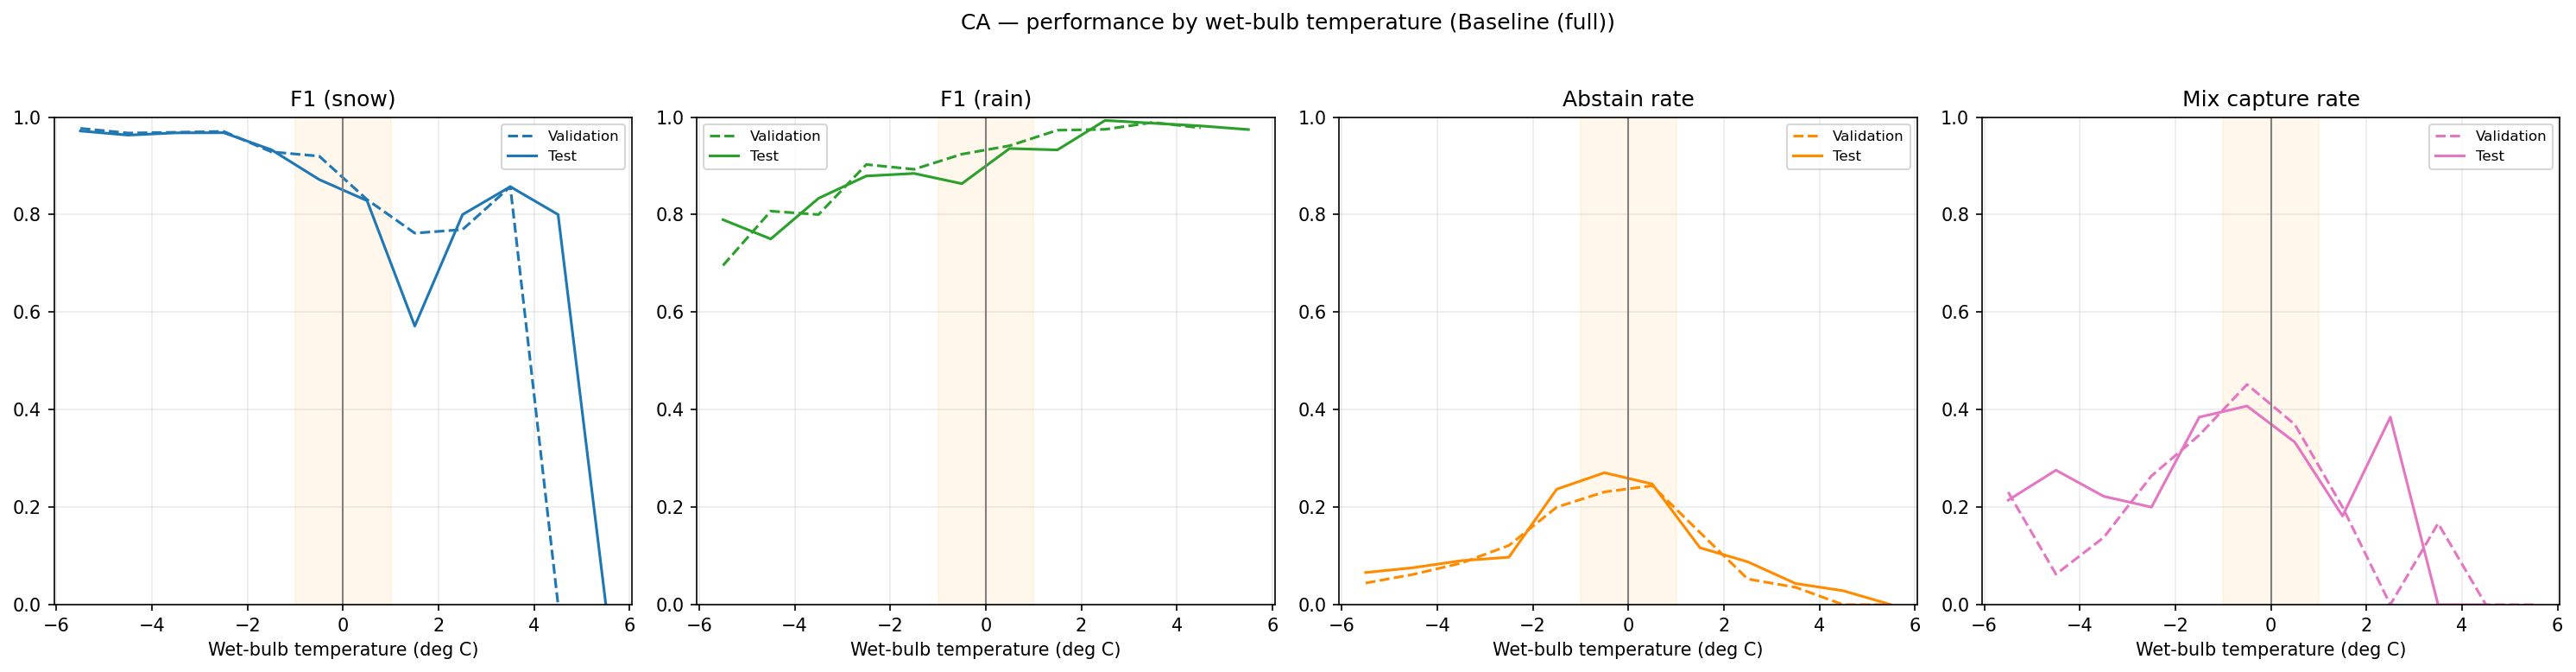
\includegraphics[width=0.95\textwidth]{CA/CA_f1_by_wetbulb.png}\\[2pt]
  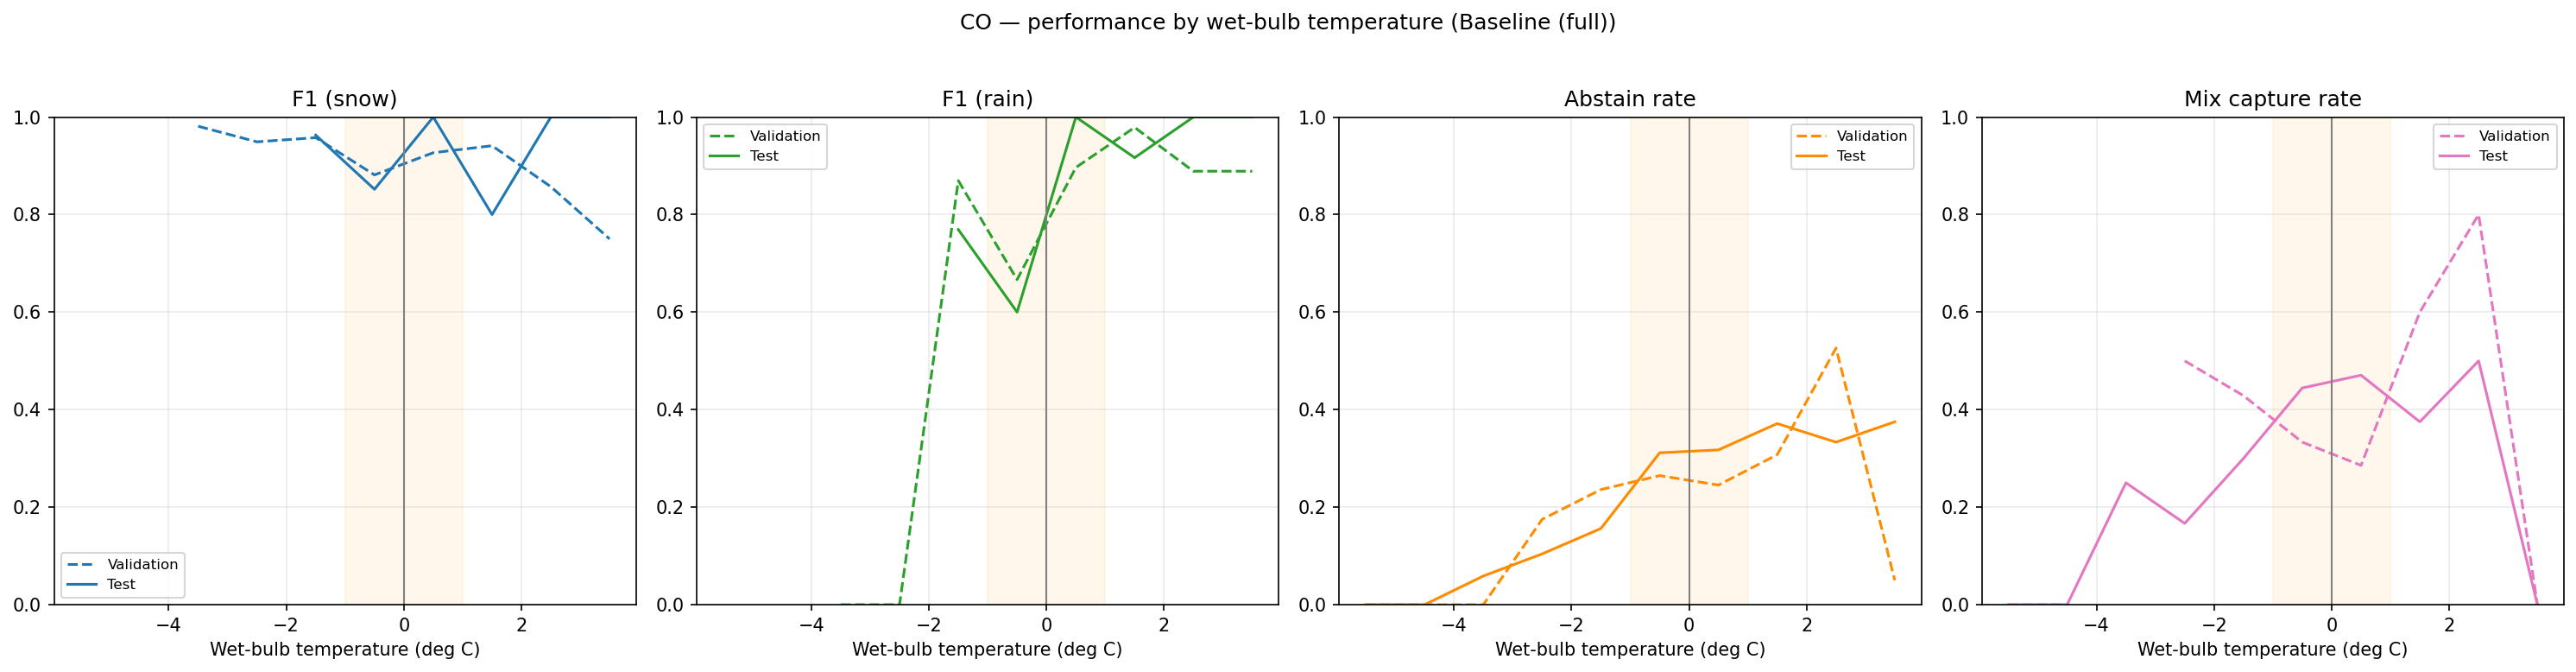
\includegraphics[width=0.95\textwidth]{CO/CO_f1_by_wetbulb.png}
  \caption{Per-phase F1, flag rate, and mix-capture rate in \degC{1} wet-bulb
  bins for California (top) and Colorado (bottom), validation (dashed)
  and test (solid). Shading marks $|T_w| \le \degC{1}$; bins span
  \degC{-6} to \degC{6} and are plotted at midpoints. Skill is lowest,
  and the uncertainty envelope most valuable, in the near-freezing
  transition zone.
  %
  The F1 panels count only observations the model committed to, so they
  must be read against the flag-rate panel: a high F1 bought by frequent
  abstention is not the same result as a high F1 at full coverage. Line
  breaks mark undefined or under-sampled statistics rather than gaps in
  the analysis window. F1 is undefined where a bin's committed sample
  holds only one phase, which causes the breaks below \degC{-2} in
  Colorado, and bins with fewer than 10 observations are dropped, which
  truncates Colorado's warm tail near \degC{3.5}. A plotted zero, by
  contrast, is a real failure to recover a phase that was present.}
  \label{fig:twet}
\end{figure*}


\subsection{Input-dependent skill}
\label{sec:ablation-results}
Our first research question asks whether the assimilated predictors
contribute skill beyond thermodynamics. We answer it in two steps: which
features the fitted model uses, then which it needs.

\paragraph{Feature attribution.}
SHAP attributions show that the two domains lean on different predictors
(Figures~\ref{fig:app-shap} and~\ref{fig:shap-wetbulb}). California is
led by the leakage-safe MRoS surfaces and elevation, with the raw
temperatures contributing surprisingly little, whereas Colorado is led by
IMERG pLP and air temperature. Both shift reliance toward the phase
boundary: usage rises near freezing for exactly the predictors that
resolve ambiguity, among them the interpolated MRoS mix surface, even
though observer-reported mix is withheld from training. That mixed
observations register at all, having been discarded in prior work, is
itself worth noting.

Attribution cannot settle whether a predictor is \emph{needed}, however,
because it describes only how the fitted model distributes credit among
inputs that are themselves strongly correlated: the crowdsourced
surfaces partly re-encode the thermodynamics they appear to displace, so
their high attribution and the temperatures' low attribution are two
sides of the same accounting. Retraining answers the question directly.

\paragraph{Ablation.}
Retraining under the six configurations of Table~\ref{tab:ablation}
confirms that the assimilated predictors carry unique information in
both domains, through complementary channels. In California, removing
the MRoS surfaces is the most damaging single ablation and
thermodynamics alone is worse still. In Colorado no single-feature
removal moves macro F1 by more than 0.01 and every interval overlaps the
baseline's, so only the thermodynamics-only collapse is visible in the
absolute values, and the rest we defer to the paired differences below.
In both domains a compact minimal core of wet-bulb temperature,
elevation, the MRoS surfaces, and IMERG pLP nearly matches the full
model, indicating that a lean feature set is deployable.

The paired differences (Figure~\ref{fig:ablation-ci}) turn this into
causal claims and locate them near freezing. In California the MRoS
surfaces are worth 9.6 points of near-freezing accuracy (6.5--12.7),
and the five non-thermodynamic predictors together are
worth 15.7 points (12.2--19.4), both on every metric. Three refinements
emerge that the absolute values obscured. No single temperature is worth
a measurable amount on overall accuracy, macro F1 or AUROC, confirming
that the three substitute for one another, with one exception: wet-bulb
temperature is worth 1.7 near-freezing points (0.4--3.0), so the
substitution holds in aggregate but not at the phase boundary. Elevation
matters more than the absolute values suggested, contributing measurably
on every metric. And IMERG pLP earns its place specifically near
freezing, worth 1.9 near-freezing points (0.5--3.3) while its overall
contribution stays within noise. Colorado separates fewer effects: the
non-thermodynamic predictors are worth 11.2 near-freezing points there
(3.1--19.5) and register on every metric, the MRoS surfaces register on
overall AUROC alone, and pLP only on near-freezing AUROC, the same
near-freezing role it plays in California.

Near-freezing AUROC makes the aggregate case. It rises from 0.796
(0.761--0.830) in California and 0.791 (0.715--0.862) in Colorado under
thermodynamics-only to 0.922 and 0.920 for the full model, a gain of
0.126 (0.096--0.158) and 0.129 (0.066--0.196). Feature effects
concentrate where the problem is hard.

Resolving the MRoS ablation against temperature
(Figures~\ref{fig:mros-contrib} and~\ref{fig:mros-contrib-tair})
localizes that loss to a specific error: without the crowdsourced
surfaces California's near-freezing snow recall halves, from 0.44 to 0.22
at $T_w = \degC{1.5}$, so the observer network is what prevents
near-freezing snow from being misread as rain. Colorado's curves cross
within sampling noise, matching its weaker interval-based result.


\begin{figure*}[tp]
  \centering
  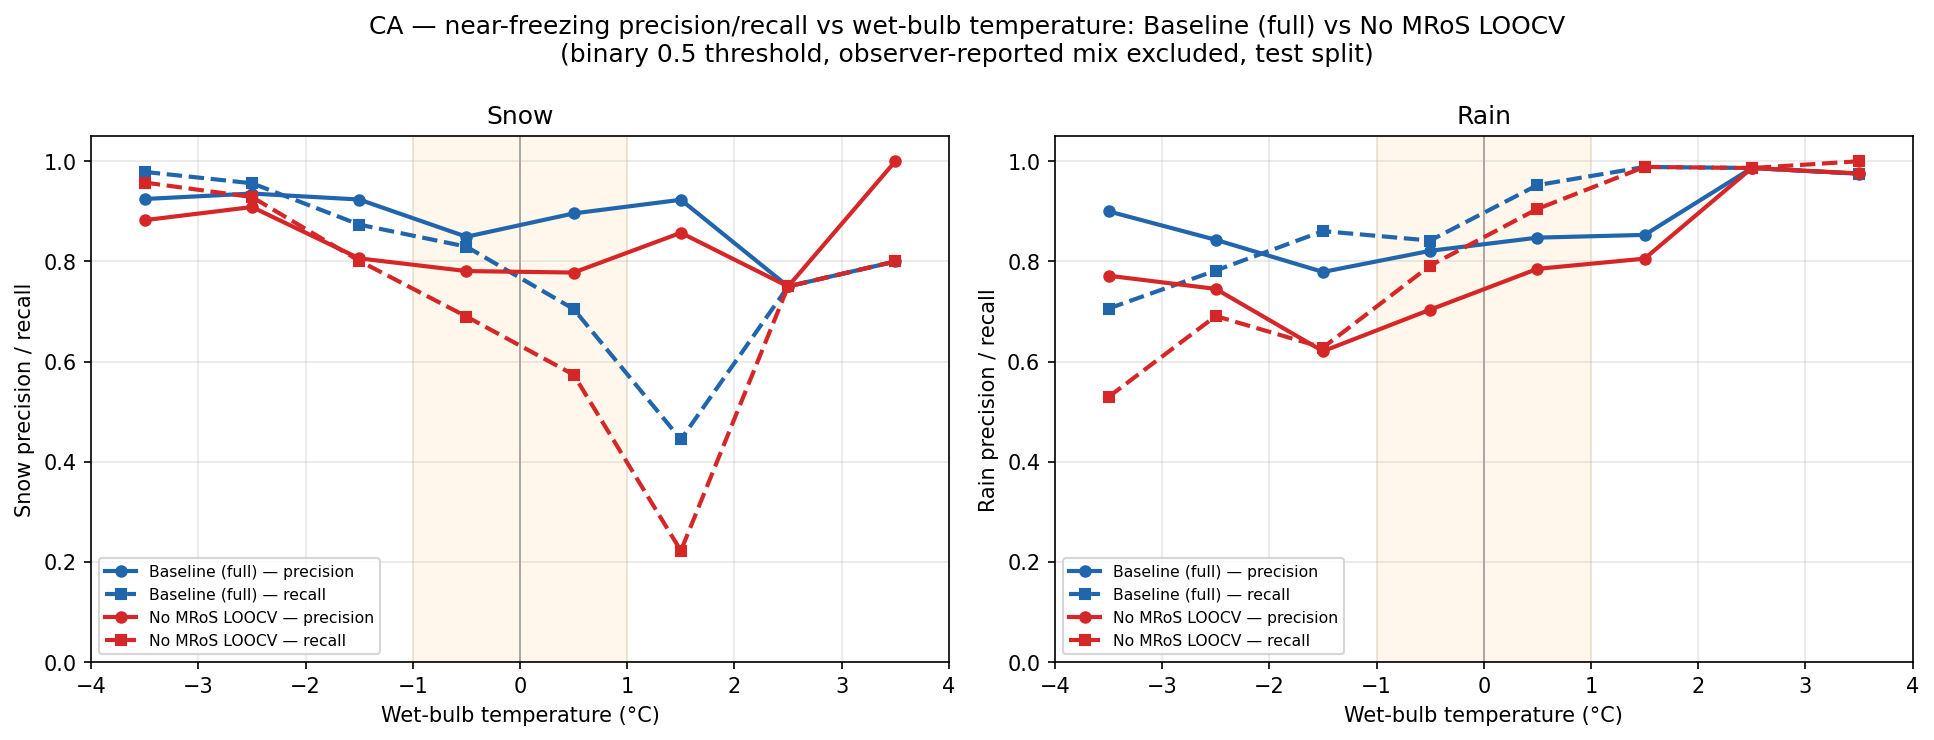
\includegraphics[width=0.95\textwidth]{CA/CA_story5_nearfreeze_twet_comparison.png}\\[2pt]
  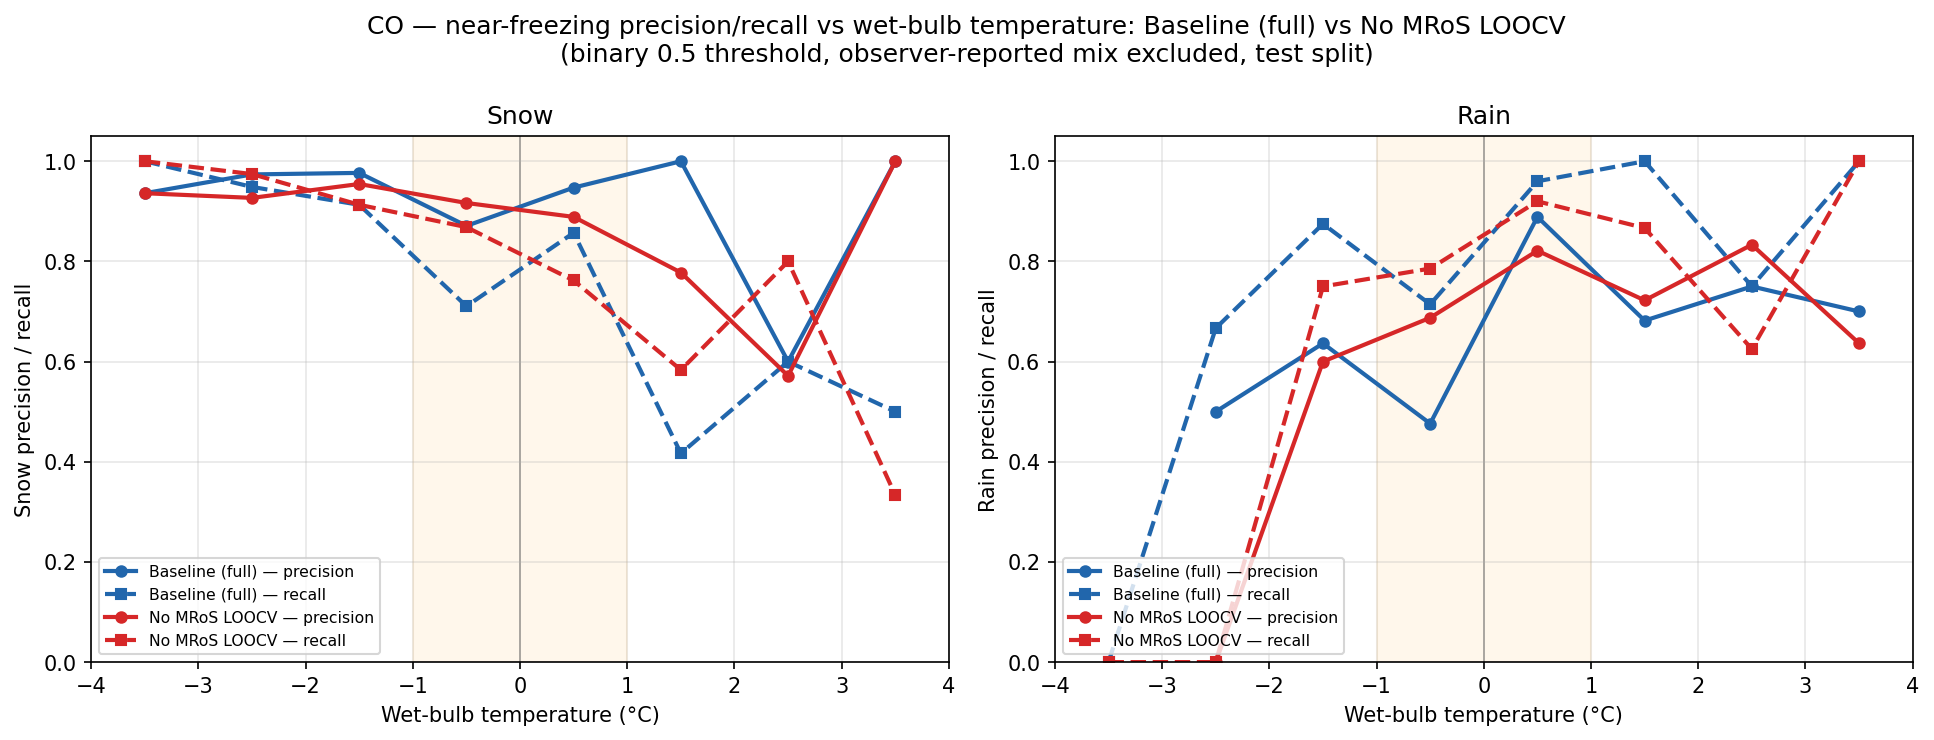
\includegraphics[width=0.95\textwidth]{CO/CO_story5_nearfreeze_twet_comparison.png}
  \caption{What the crowdsourced surfaces contribute at the phase boundary:
  near-freezing precision and recall against wet-bulb temperature for the
  full model (blue) and the same model with the MRoS surfaces removed
  (red), for California (top) and Colorado (bottom), snow (left) and rain
  (right). Held-out test split, scored at the raw $0.5$ threshold with no
  uncertainty band applied, so the comparison isolates the predictor
  contribution rather than the abstention rule; mix is excluded and
  shading marks $|T_w| \le \degC{1}$.
  %
  In California the crowdsourced surfaces are what keeps the model usable
  through the transition: snow recall at $T_w = \degC{1.5}$ falls from
  $0.44$ to $0.22$ without them. Because these are recall curves at a
  fixed threshold, the loss appears as snow missed and called rain, which
  is the failure mode that matters hydrologically. Colorado does not
  reproduce the pattern; its curves cross repeatedly, but with 179
  near-freezing observations the crossings are well inside sampling
  noise, and the interval-based ablation of Table~\ref{tab:ablation} is
  the appropriate test. Figure~\ref{fig:mros-contrib-tair} repeats the
  comparison against air temperature.}
  \label{fig:mros-contrib}
\end{figure*}

\begin{table*}[tp]
  \centering
  \scriptsize
  \caption{Ablation study: held-out test performance by feature configuration,
  with 95\% cluster-bootstrap confidence intervals. Configurations retain the
  following predictors, where $T_a$, $T_d$ and $T_w$ are air, dewpoint and
  wet-bulb temperature, Elev is elevation, pLP is the IMERG probability of
  liquid precipitation, and MRoS denotes the three leakage-safe MRoS phase
  surfaces, counted as three predictors. \emph{Baseline (full)}: all eight
  ($T_a$, $T_d$, $T_w$, Elev, pLP, MRoS). \emph{No MRoS surfaces}: five
  ($T_a$, $T_d$, $T_w$, Elev, pLP). \emph{No IMERG pLP}: seven ($T_a$, $T_d$,
  $T_w$, Elev, MRoS). \emph{No elevation}: seven ($T_a$, $T_d$, $T_w$, pLP,
  MRoS). \emph{Thermodynamics only}: three ($T_a$, $T_d$, $T_w$).
  \emph{Minimal core}: six ($T_w$, Elev, pLP, MRoS). All configurations use
  kriged predictors, beta calibration, and identical splits. Single-predictor
  removals of $T_a$, $T_d$ and $T_w$ were also run and are discussed in
  Section~\ref{sec:ablation-results}. NF = near-freezing ($|T_w| \le \degC{2}$).}
  \label{tab:ablation}
  \begin{tabular}{llcccc}
    \topline
    Domain & Configuration & ROC AUC & Macro F1 & NF ROC AUC & Mix capture \\
    \midline
    CA & Baseline (full) & .965 (.957--.973) & .905 (.891--.919) & .922 (.902--.941) & .30 (.24--.36) \\
    CA & No MRoS surfaces & .936 (.925--.947) & .850 (.832--.867) & .861 (.835--.888) & .34 (.28--.40) \\
    CA & No IMERG pLP & .964 (.956--.972) & .899 (.885--.913) & .916 (.895--.936) & .29 (.24--.35) \\
    CA & No elevation & .956 (.947--.964) & .887 (.873--.902) & .905 (.882--.926) & .33 (.28--.38) \\
    CA & Thermodynamics only & .907 (.892--.921) & .817 (.797--.836) & .796 (.761--.830) & .49 (.43--.55) \\
    CA & Minimal core & .966 (.958--.973) & .900 (.885--.914) & .922 (.902--.941) & .32 (.26--.37) \\
    \midline
    CO & Baseline (full) & .965 (.941--.982) & .867 (.820--.906) & .920 (.864--.962) & .33 (.21--.45) \\
    CO & No MRoS surfaces & .948 (.916--.973) & .863 (.820--.903) & .896 (.836--.946) & .31 (.20--.43) \\
    CO & No IMERG pLP & .959 (.935--.978) & .871 (.825--.910) & .903 (.841--.951) & .31 (.20--.43) \\
    CO & No elevation & .959 (.936--.977) & .862 (.818--.901) & .912 (.857--.956) & .34 (.22--.47) \\
    CO & Thermodynamics only & .925 (.897--.951) & .798 (.746--.846) & .791 (.715--.862) & .53 (.40--.65) \\
    CO & Minimal core & .963 (.940--.981) & .862 (.816--.903) & .924 (.873--.965) & .39 (.26--.52) \\
    \botline
  \end{tabular}
\end{table*}

% NOTE: the relative-improvement CI figure is now included as
% Fig.~\ref{fig:relimp} (appendix). Fig.~\ref{fig:forest} is retained
% because Table~\ref{tab:benchmark} gives per-method CIs but not the
% paired model-minus-benchmark differences the significance claims rest on.
\subsection{Comparison against operational partitioning methods}
\label{sec:bench-results}
MRoS-XGB outperformed all nine benchmarks in both domains
(Table~\ref{tab:benchmark}), and the margin widens near freezing
(Figure~\ref{fig:tair}; the same comparison in difference form is
Figure~\ref{fig:relimp}). In California its accuracy was 91.2\% against
80.1\% for the best benchmark, a dewpoint threshold at
$T_d = \degC{0.0}$, and 85.6\% against 69.1\% near freezing. In
Colorado it was 91.4\% against 87.8\% for $T_d = \degC{0.5}$, and
82.7\% against 74.3\% near freezing. The benchmark ordering reproduces
\citet{jennings2025}, with air-temperature-only thresholds worst and
humidity-aware thresholds intermediate.

Paired differences show these gaps are not artifacts of the test draw
(Figure~\ref{fig:forest}). In California all 36 differences, across nine
benchmarks and four metrics, are positive and clear of zero. No resample
out of 5{,}000 favored a benchmark, giving $p < 0.0002$, which is the
smallest value 5{,}000 resamples can resolve. Against the best benchmark
MRoS-XGB gains 11.1 points of accuracy overall (9.0--13.4) and 16.5 near
freezing (12.2--21.1), so even at the interval floors it is at least nine
points better overall and twelve better near freezing than the strongest
method in the suite.

Colorado is consistent but tighter, and there the choice of metric
matters. Thirty-five of its 36 differences clear zero. On overall
accuracy the gain against $T_d = \degC{0.5}$ is 3.6 points (0.2--6.9,
$p = 0.021$), and the near-freezing accuracy gain of 8.4 points ($-0.6$
to $+16.9$) is the one difference that does not, although
96\% of resamples still favored MRoS-XGB ($p = 0.037$). On macro F1
every Colorado difference clears zero ($p \le 0.0002$), because macro
F1 weights rain equally and so exposes the collapse in benchmark rain
recall that accuracy conceals where 82\% of observations are snow.
Against $T_d = \degC{0.5}$, whose rain recall is 0.531 against
MRoS-XGB's 0.865 (Table~\ref{tab:benchmark}), the macro F1 gain is
0.096 (0.042--0.152). The domains thus tell one story at different
strengths, decisive where the observer network is dense and, where it is
sparse, decisive on the balanced metric while borderline on the metric
the majority class dominates.

\paragraph{Phase bias.}
A method can reach respectable accuracy while systematically mistaking
one phase for the other, and the benchmarks do. Near freezing in
California, the $T_a = \degC{1.0}$ threshold calls snow 76\% less often
than it occurred and rain 73\% more often, while the wet-bulb thresholds
fail by a similar margin in the opposite direction
($T_w = \degC{1.0}$: 74\% too much snow, 71\% too little rain). Because
these two errors partly cancel, the accuracy figure alone conceals them,
which is why we report phase bias beside it.

Only two California methods predict each phase about as often as it
occurred: MRoS-XGB and the \citet{jennings2018spatial} logistic applied
without refitting. Comparing them is instructive. The transferred
logistic gets the totals right yet is correct on only 72\% of individual
events, so it is right on average and wrong case by case, whereas
MRoS-XGB matches the totals at 91\% accuracy. Predicting the right
amount of snow is not the same as predicting it on the right days, and
only the latter is useful for forcing a hydrologic model.
Figure~\ref{fig:tair-bias} resolves these biases against air
temperature for the full benchmark suite, showing that each threshold's
error reverses sign across its own threshold, so a method can appear
accurate in a bin while being badly biased in both phases within it.

\paragraph{Sensitivity to cluster geometry.}
Because the cluster geometry is constructed post hoc
(Section~\ref{sec:uq}), we verified that it does not drive the
conclusions. Intervals are essentially identical across 15-, 30-, and
60-km blocks, with California delta-CI widths of 0.042 to 0.044, and
are 13 to 28\% wider than an i.i.d. bootstrap would give (28\% for the
California headline delta, 14\% for Colorado's). The clustering
correction therefore mattered, but no conclusion flips between i.i.d.
and clustered resampling, and none depends on the block size chosen.


\begin{table*}[tp]
  \centering
  \scriptsize
  \caption{Held-out test performance of the model and the nine benchmark
  partitioning methods, with 95\% cluster-bootstrap confidence intervals
  (5{,}000 resamples; 30-km $\times$ calendar-day clusters). Methods are
  ordered by overall accuracy within each domain. NF = near-freezing subset
  ($|T_w| \le \degC{2}$; $n = 782$ in CA, $n = 179$ in CO). Point estimates are
  computed once on the full test set and are not medians over resamples, so
  intervals need not be symmetric about them. Per-phase recall and bias with
  intervals are given for the model in Table~\ref{tab:bootstrap}. Paired
  model-minus-benchmark differences, which are the basis for the significance
  claims in Section~\ref{sec:bench-results}, appear in
  Figure~\ref{fig:forest}.}
  \label{tab:benchmark}
  \begin{tabular}{llcccc}
    \topline
    Domain & Method & Accuracy (\%) & Macro F1 & NF accuracy (\%) & NF macro F1 \\
    \midline
    CA & MRoS-XGB (this study) & \textbf{91.2 (89.9--92.5)} & \textbf{.905 (.891--.920)} & \textbf{85.6 (82.9--88.3)} & \textbf{.855 (.828--.882)} \\
    CA & $T_d = \degC{0.0}$ & 80.1 (77.9--82.2) & .781 (.757--.802) & 69.1 (65.2--72.8) & .689 (.651--.726) \\
    CA & $T_d = \degC{0.5}$ & 79.1 (76.8--81.2) & .756 (.732--.779) & 68.5 (64.6--72.3) & .676 (.637--.713) \\
    CA & $T_w = \degC{0.0}$ & 75.5 (73.0--77.9) & .698 (.671--.725) & 62.4 (58.7--66.2) & .618 (.580--.655) \\
    CA & $T_w = \degC{0.5}$ & 74.8 (72.3--77.3) & .675 (.648--.702) & 60.5 (56.6--64.4) & .577 (.538--.616) \\
    CA & Bin.\ logistic (refit) & 73.8 (71.1--76.4) & .700 (.672--.727) & 60.0 (56.1--63.9) & .598 (.558--.636) \\
    CA & $T_w = \degC{1.0}$ & 73.6 (70.9--76.2) & .645 (.617--.674) & 56.8 (52.7--61.0) & .510 (.472--.550) \\
    CA & Bin.\ logistic (transferred) & 72.0 (69.3--74.6) & .697 (.670--.723) & 59.5 (55.6--63.4) & .581 (.541--.620) \\
    CA & $T_a = \degC{1.5}$ & 64.8 (62.0--67.5) & .645 (.618--.672) & 57.0 (53.0--61.1) & .514 (.475--.552) \\
    CA & $T_a = \degC{1.0}$ & 62.0 (59.2--64.8) & .620 (.592--.647) & 55.1 (51.0--59.4) & .469 (.432--.508) \\
    \midline
    CO & MRoS-XGB (this study) & \textbf{91.4 (88.4--94.1)} & \textbf{.867 (.821--.906)} & \textbf{82.7 (76.4--88.3)} & \textbf{.820 (.753--.877)} \\
    CO & $T_d = \degC{0.5}$ & 87.8 (84.7--90.8) & .771 (.717--.818) & 74.3 (67.2--81.3) & .692 (.614--.761) \\
    CO & $T_w = \degC{0.5}$ & 86.5 (82.7--89.9) & .763 (.706--.816) & 70.4 (62.4--77.7) & .651 (.563--.732) \\
    CO & $T_d = \degC{0.0}$ & 86.3 (82.7--89.7) & .769 (.719--.816) & 71.5 (64.3--78.7) & .684 (.610--.755) \\
    CO & $T_w = \degC{0.0}$ & 86.1 (82.1--89.8) & .780 (.726--.832) & 69.3 (60.8--77.1) & .673 (.586--.754) \\
    CO & $T_w = \degC{1.0}$ & 85.3 (81.5--88.8) & .718 (.658--.774) & 67.0 (59.1--74.9) & .559 (.473--.646) \\
    CO & Bin.\ logistic (refit) & 84.0 (80.1--87.7) & .677 (.618--.737) & 63.7 (55.8--71.4) & .514 (.439--.593) \\
    CO & $T_a = \degC{1.5}$ & 81.3 (77.0--85.5) & .747 (.695--.796) & 58.1 (50.3--66.1) & .581 (.500--.660) \\
    CO & Bin.\ logistic (transferred) & 80.7 (76.1--85.2) & .740 (.690--.790) & 57.5 (49.5--65.8) & .575 (.492--.655) \\
    CO & $T_a = \degC{1.0}$ & 79.2 (74.6--83.6) & .739 (.687--.788) & 54.2 (45.9--62.4) & .537 (.453--.618) \\
    \botline
  \end{tabular}
\end{table*}

\begin{figure*}[tp]
  \centering
  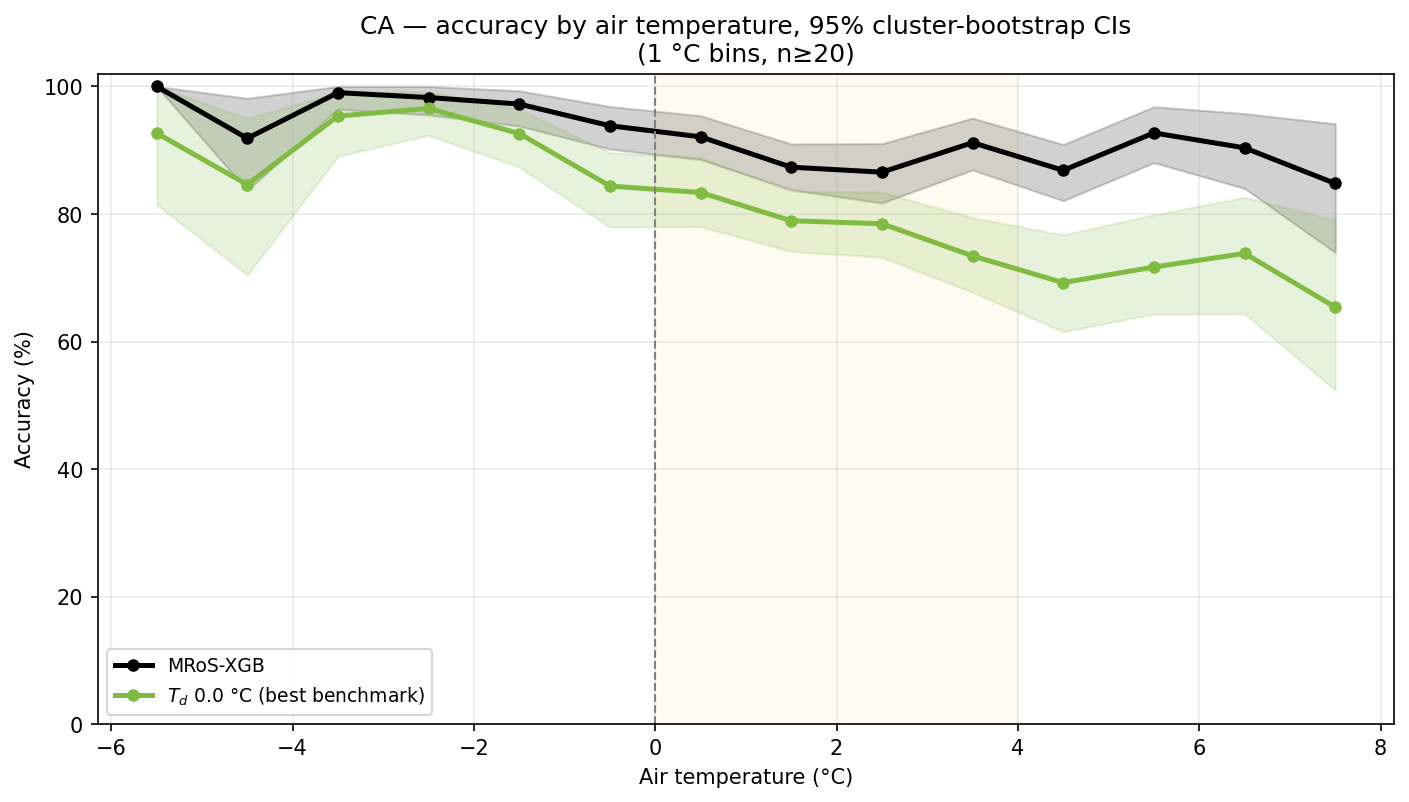
\includegraphics[width=0.49\textwidth]{CA/CA_benchmark_accuracy_by_tair_ci.png}
  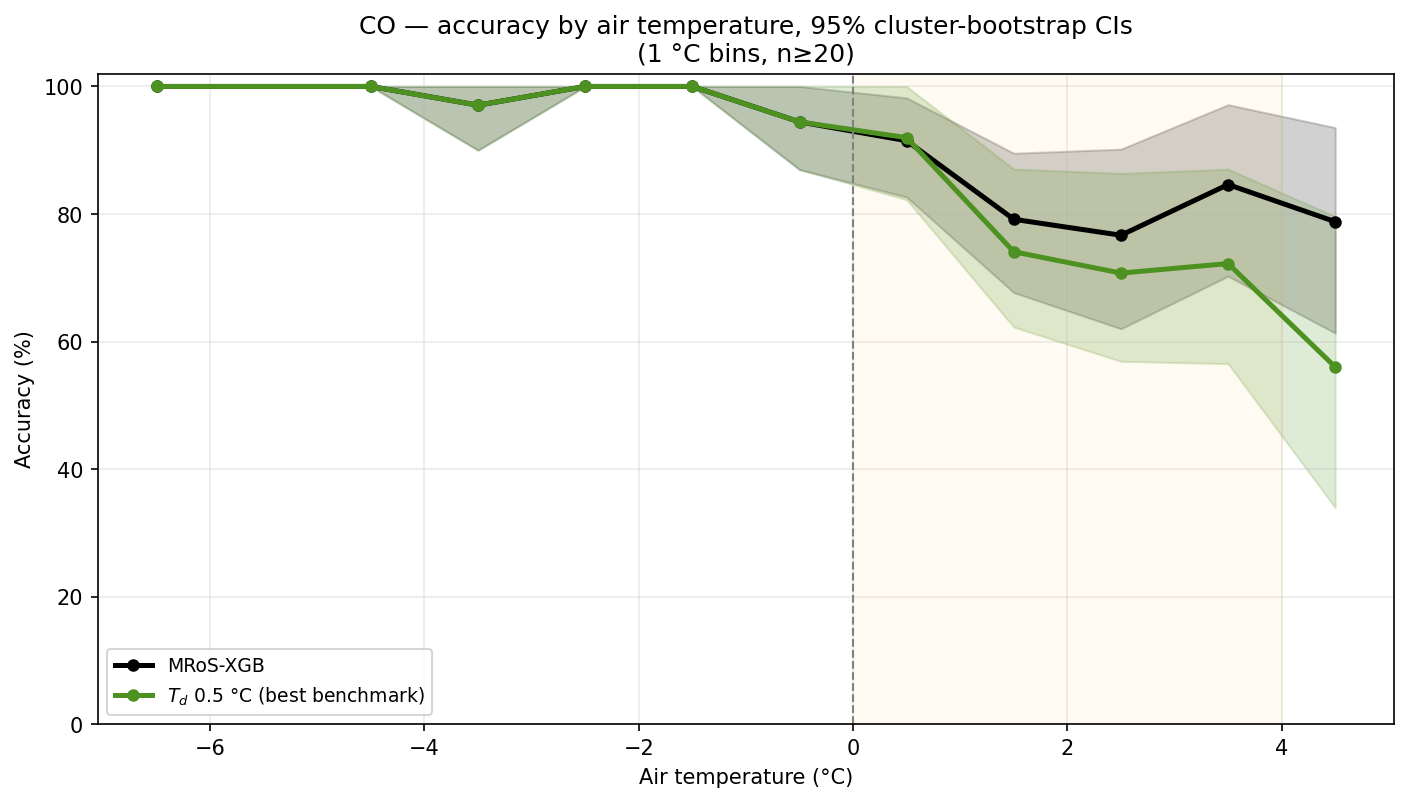
\includegraphics[width=0.49\textwidth]{CO/CO_benchmark_accuracy_by_tair_ci.png}
  \caption{Held-out accuracy by air temperature bin for MRoS-XGB (black) and the
  best benchmark in each domain (blue), with 95\% cluster-bootstrap
  confidence bands, for California (left) and Colorado (right). The
  shaded \degC{0}--\degC{4} region marks the climatologically ambiguous
  zone, where the model's advantage grows precisely as threshold methods
  lose skill.
  %
  Accuracy is evaluated on rain and snow observations in \degC{1} bins
  plotted at midpoints, with bins holding fewer than 20 observations
  dropped, which is why the curves stop short of the nominal range at
  both tails. Ribbons are 2.5th--97.5th percentiles of 500
  cluster-bootstrap resamples over \mbox{30-km} $\times$ calendar-day
  blocks. Resampling at cluster level makes these intervals wider than
  naive binomial ones, which is the honest choice given that nearby
  simultaneous reports are not independent; the 500 resamples used here,
  against 5{,}000 for the scalar metrics, make the tails grainier.
  ``Best benchmark'' is chosen per domain, so it is not necessarily the
  same method in both panels.}
  \label{fig:tair}
\end{figure*}

\begin{figure*}[tp]
  \centering
  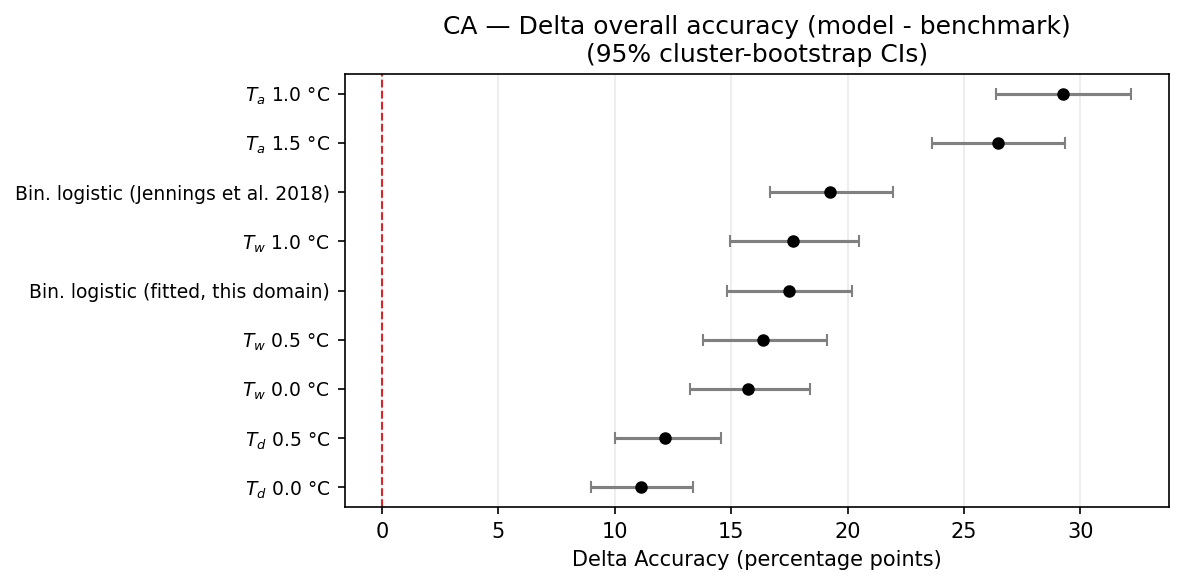
\includegraphics[width=0.49\textwidth]{CA/CA_benchmark_delta_forest.png}
  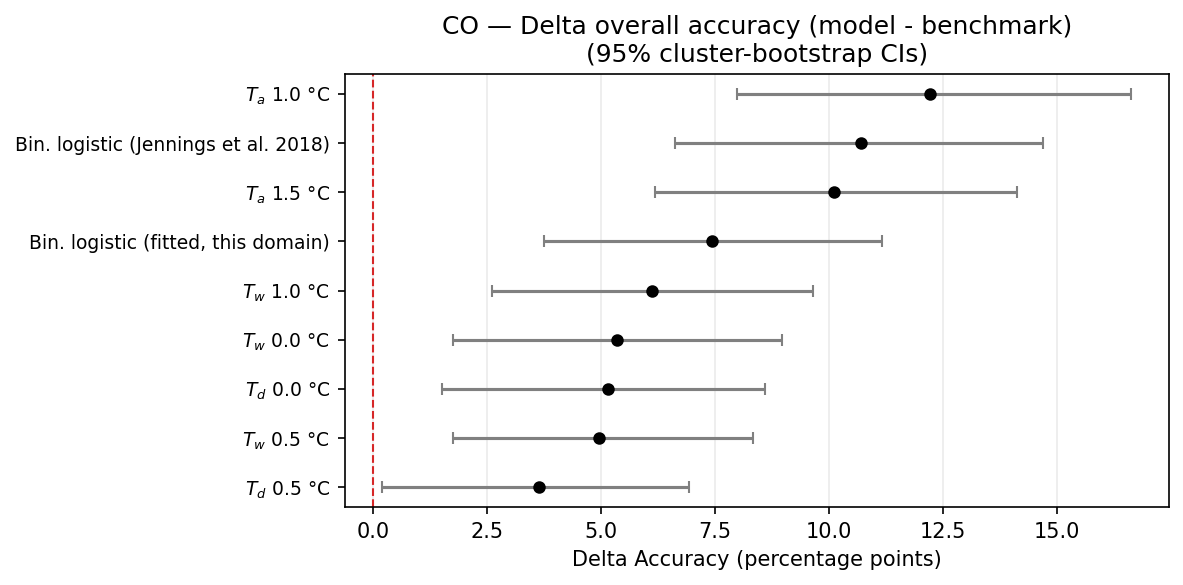
\includegraphics[width=0.49\textwidth]{CO/CO_benchmark_delta_forest.png}\\[2pt]
  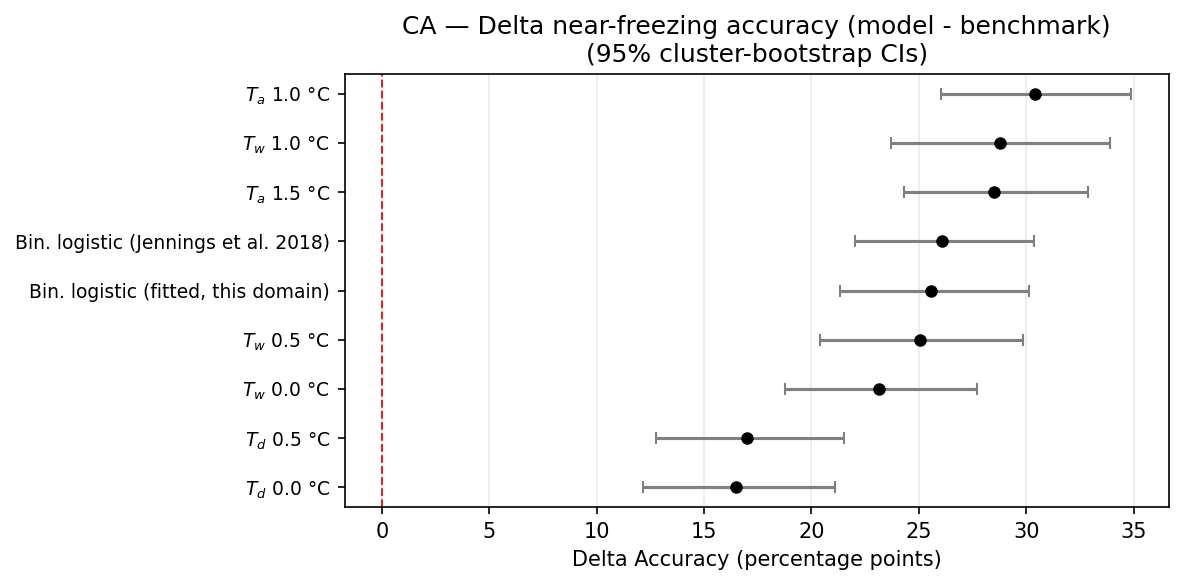
\includegraphics[width=0.49\textwidth]{CA/CA_benchmark_delta_forest_nearfreeze.png}
  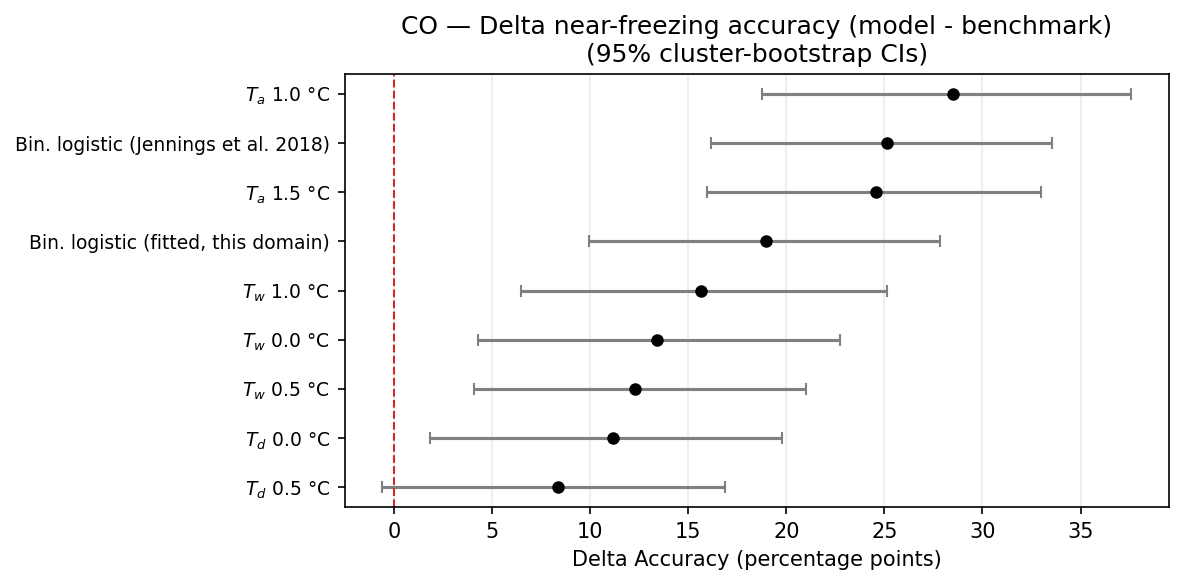
\includegraphics[width=0.49\textwidth]{CO/CO_benchmark_delta_forest_nearfreeze.png}
  \caption{Paired model-minus-benchmark accuracy differences with 95\%
  cluster-bootstrap confidence intervals: overall (top) and near-freezing
  (bottom) for California (left) and Colorado (right). Every California
  interval lies entirely above zero. In Colorado all overall intervals do
  too, and only the near-freezing difference against $T_d = \degC{0.5}$
  reaches back across it.
  %
  Differences are paired within each resample, so each interval reflects
  the variability of the \emph{difference} on common data rather than of
  two independently resampled quantities, which is the correct
  construction because model and benchmark are scored on identical
  observations. Intervals are 2.5th--97.5th percentiles of 5{,}000
  resamples over \mbox{30-km} $\times$ calendar-day clusters; the
  near-freezing subset is $|T_w| \le \degC{2}$ ($n = 782$ in California,
  $n = 179$ in Colorado). These intervals quantify test-set sampling
  uncertainty only: they do not propagate uncertainty in the kriged
  surfaces, nor retraining variability, either of which would widen
  them.}
  \label{fig:forest}
\end{figure*}


\subsection{The mixed-phase uncertainty envelope}
\label{sec:mix-results}
The third research question asks whether mixed precipitation can be
represented as a region of model uncertainty, which requires that the envelope fall where mixed
precipitation actually occurs. It does, in the aggregate sense. The
flag rate peaks near $T_w = \degC{0}$ in both domains
(the abstain-rate panels of Figure~\ref{fig:twet}), so the model
concentrates its uncertainty in the physically ambiguous regime without
having been told where that regime is. Figure~\ref{fig:band} shows the
fitted envelope against the mixed events themselves, and
Figure~\ref{fig:mix-capture} resolves capture into wet-bulb bins.

Against individual events the result is partial. The envelope captured
30\% (95\% CI 25--36\%) of observer-reported mix events in California
and 33\% (21--45\%) in Colorado, and most misses were assigned confident
extreme probabilities ($p > 0.8$ or $p < 0.2$). Captured and missed
events are distributed differently in the two domains
(Figure~\ref{fig:band}): in California they span a wide range of
temperature and probability, suggesting meteorological ambiguity, whereas
in Colorado captured events cluster near $p \approx 0.5$--$0.65$ and
$T_w \in [-1, +2]\,^{\circ}$C. For context, every benchmark and the
machine-learning methods of \citet{jennings2025} capture 0\%, because
none incorporate mix phase or flag uncertainty. We read capture below 50\% not as
classifier failure but as evidence bearing on whether observer-reported
mix is a coherent, learnable category
(Section~\ref{sec:discussion}).

% TODO: revist this paragraph and consolidate
The envelope width is not a free choice but the optimum of an explicit
tradeoff. Sweeping the three band parameters over the validation set
traces a frontier between mix capture and confident rain--snow coverage.
The adopted configuration ($b = 0.20$, $a = 0.15$,
$\sigma = \degC{2.0}$) maximizes the composite objective in California
at a validation capture rate of 0.36 while retaining 90\% coverage at
94.4\% accuracy on the calls it makes. That figure is not comparable to
the 91.2\% headline accuracy, which scores every rain--snow observation
including those the envelope would have flagged
(Section~\ref{sec:eval-framework}). Neighboring configurations trade the
two monotonically: holding $a$ and $\sigma$ fixed, narrowing $b$ to 0.15
raises California coverage to 0.92 while capture drops to 0.26, and
$b = 0.10$ raises it to 0.94 as capture falls to 0.20. Colorado traces
the same frontier at uniformly lower capture (0.25 at the adopted
setting), consistent with its smaller mixed-event sample. Reporting the
frontier rather than a single tuned point makes the operating choice
auditable and lets users re-tune toward sensitivity or precision as an
application demands.

\begin{figure*}[tp]
  \centering
  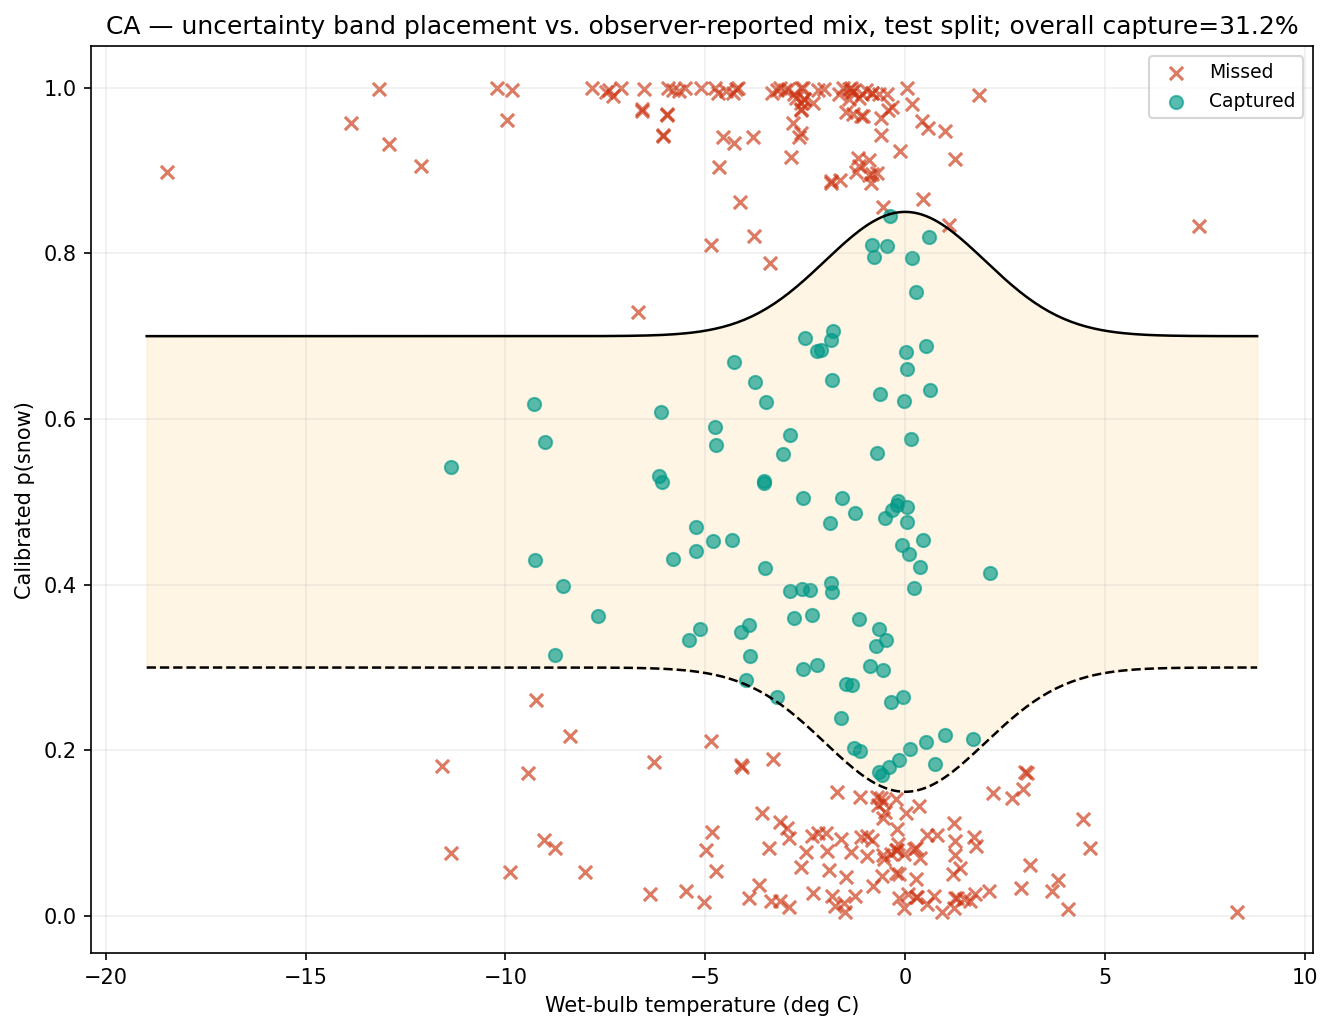
\includegraphics[width=0.72\textwidth]{CA/CA_band_placement_appendix.png}\\[2pt]
  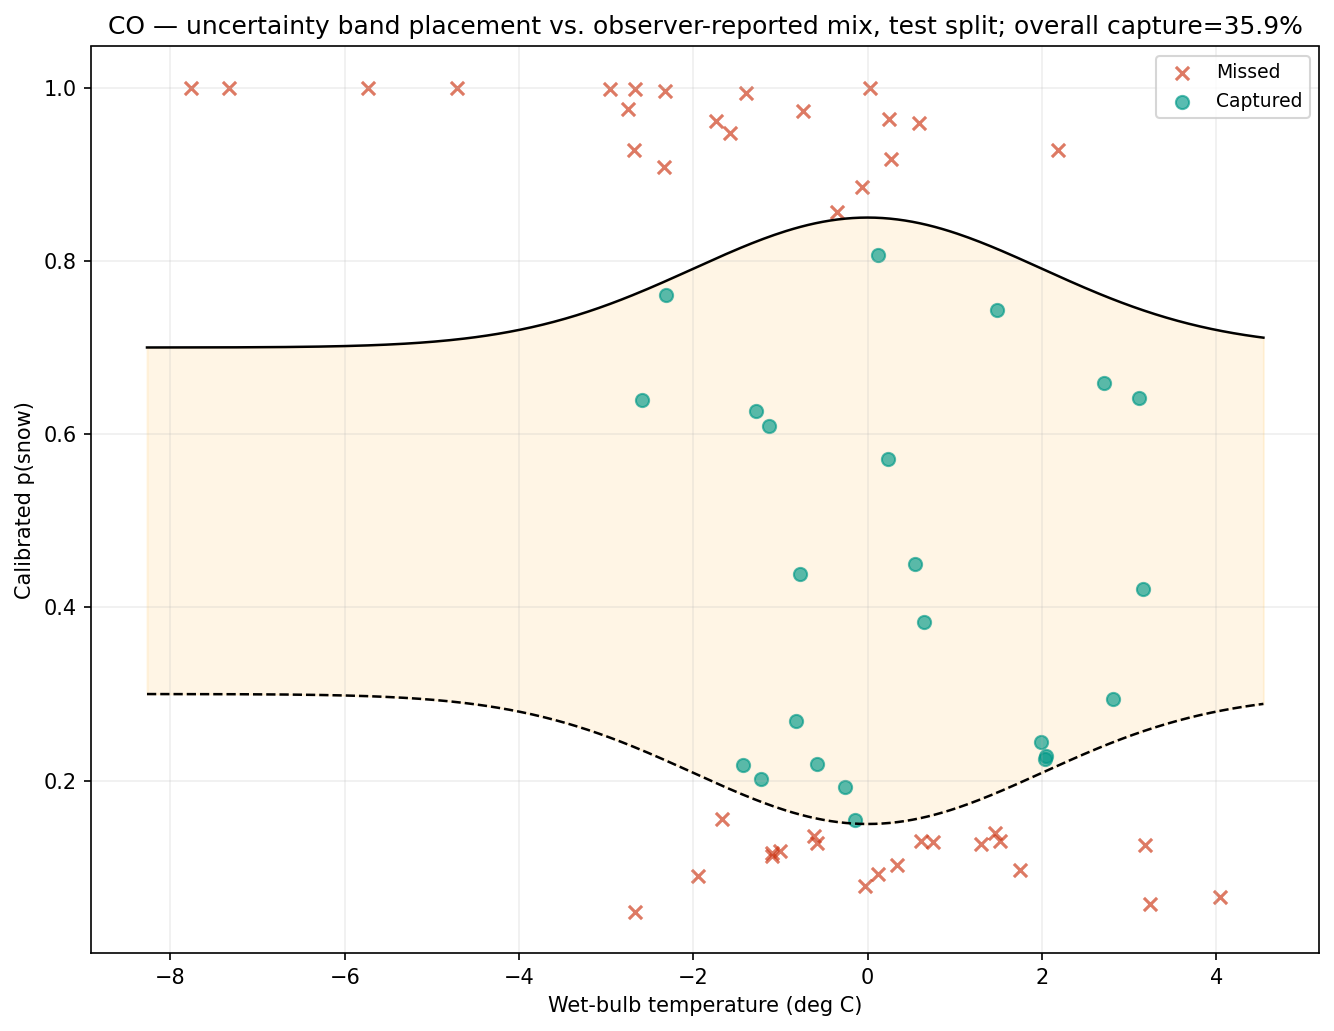
\includegraphics[width=0.72\textwidth]{CO/CO_band_placement_appendix.png}
  \caption{The fitted uncertainty envelope and where observer-reported mixed
  events fall relative to it, for California (top) and Colorado (bottom),
  held-out test split. Solid and dashed curves are the snow and rain
  thresholds of Equation~\ref{eq:band}: the shaded interior is the
  envelope, $0.30/0.70$ at both temperature extremes and opening to
  $0.15/0.85$ at $T_w = \degC{0}$. Each marker is one mixed event,
  filled where the envelope captured it and crossed where it did not.
  Mix was withheld from training entirely, so every marker is an
  out-of-sample test.
  %
  Two features carry the argument. Captured events concentrate where the
  envelope is widest, near \degC{0}, which is the behavior the
  construction was meant to produce. And the misses are overwhelmingly
  \emph{not} near-misses: they sit against $p(\mathrm{snow}) \approx 0$
  or $\approx 1$, meaning the model was confident and wrong rather than
  marginally short of the threshold. Widening the band would therefore
  recover few of them while sacrificing confident rain--snow coverage,
  the tradeoff quantified in Section~\ref{sec:mix-results}.
  Figure~\ref{fig:mix-capture} resolves the same events by wet-bulb
  bin.}
  \label{fig:band}
\end{figure*}


\subsection{Calibration case study}
\label{sec:ece-case}
Expected calibration error in California is inflated by a small,
physically interpretable cluster: 42 observations, about 0.2\% of the
data, where calibrated $p(\mathrm{snow}) < 0.05$ but the observer
reported snow. These concentrate at lower-elevation boundary sites near
1{,}570 m during marginal events in which every gridded signal points
toward rain, including the surrounding MRoS network via the
leakage-safe surface, IMERG's retrieval weighted toward lower and warmer cells, and a
near-zero wet-bulb temperature. In the Sierra Nevada the freezing level
can drop rapidly over short horizontal distances, particularly during
atmospheric river events, so an observer at 1{,}570 m may stand in snow
while stations at 1{,}400 m record rain, and interpolation across that
gradient comes out rain-dominant. Within this cluster the observer is
correct in roughly 75\% of cases. The apparent miscalibration is
therefore a property of the sparse conventional observing system rather
than a modeling failure, and it is direct evidence that citizen
observations carry non-redundant information exactly where conventional
networks do not sample.

% ======================================================================
\section{Discussion}
\label{sec:discussion}

\subsection{Implications for phase prediction}
\citet{jennings2025} found that machine learning barely improves on
threshold rules given near-surface meteorology, and our
thermodynamics-only ablation reproduces that ceiling. MRoS-XGB clears
it, and the ablations locate the difference in the assimilated
information rather than in model form, answering the first two research
questions. Both findings hold because the ceiling is set by
\emph{near-surface} information specifically: satellite pLP
senses the precipitating column that no surface instrument reaches, and
crowdsourced reports record the phase that actually arrived at the
ground. Adding either is a new observation, not a better fit to the same
predictors, and interpolation is what makes it usable, placing every
sparse source on a common grid and turning the crowdsourced reports into
a testable predictor surface rather than labels alone.

Where the observer network is dense the crowdsourced surfaces are
load-bearing; where it is sparse, satellite pLP takes over. Substituting
one source for another rather than failing outright suggests the
framework should degrade gracefully as observer density declines, which
is what matters for extending it to ranges without an established
citizen-science network. That contribution is
sharply localized: negligible away from freezing, decisive inside the
transition zone, where an individual observer is often the only
instrument at that elevation and moment, and is right about three times
in four when contradicting every gridded input the model has
(Section~\ref{sec:ece-case}).
The relationship runs both ways, since models of this type can flag
reports inconsistent with their surroundings while those reports reveal
where gridded products are biased.

Mixed precipitation, finally, is better represented as a region of model
uncertainty than as a class of its own. It has no characteristic
temperature, overlaps both end members near freezing, and collects
whatever observers cannot cleanly call, so training it as a third class
buys mostly label noise at the cost of the rain--snow boundary, while
discarding it loses the observations closest to the transition. Treating
it as uncertainty instead keeps the supervised signal clean and turns the
withheld mixed events into an independent test of where the model loses
confidence, a test no benchmark method can take because none emits a
flag at all. The flag concentrates near \degC{0} unprompted, though what
places any single observation inside the envelope, whether genuine
mixing, conflicting predictors, or sparse local data, we cannot
separate.

\subsection{Transferable methods}
Two methodological results transfer beyond precipitation phase. The
first concerns calibration. Gradient boosting on imbalanced classes
produces a model that ranks well while its stated probabilities are
unusable as probabilities, which suffices for a leaderboard but not for
hydrologic forcing or for defining an interval in probability space.
Isotonic regression, the default recommendation in much of the applied
literature, failed diagnostically on our well-separated classifier by
mapping most held-out scores to exactly 0 or 1, whereas
regime-stratified beta calibration cannot. Anyone calibrating a
well-separated, class-imbalanced Earth-science classifier should test
for that failure rather than assume the non-parametric choice is safer.

The second concerns uncertainty in clustered observations, which
describes most opportunistic and citizen-science data. Correcting for
autocorrelation costs very different amounts at different stages:
blocking the train--test split consumes training data a dataset of this
size cannot spare, whereas resampling clusters at inference only
reshapes error bars on a saved prediction table
(Section~\ref{sec:uq}). Where the correction is free it should be taken,
and here it was not cosmetic, widening intervals by up to 28\% without
flipping a conclusion. Pairing matters as much: comparing methods within
each resample, rather than across separately computed intervals, is what
made the Colorado comparison reportable at all, and it is why we can
call that result marginal rather than absent.

\subsection{Scope and limits}
The framework outputs calibrated hourly 1-km probabilities of snow and
rain with an uncertainty flag, and each property has a use. The
probabilities can replace static thresholds as phase forcing
in hydrologic and land surface models, and because they are calibrated
they can be used as probabilities rather than merely as rankings. The
flag concentrates where phase is genuinely ambiguous, which is where
rain-on-snow forecasting most needs human judgment. And the minimal-core
result matters operationally, since six predictors nearly match eight
(Table~\ref{tab:ablation}) and each one dropped is an upstream
dependency removed, IMERG latency being the main deployment risk.

The claims have boundaries. The randomized split may admit mild
within-storm leakage, so point estimates may be slightly optimistic for
a novel season; the cluster bootstrap widens intervals but cannot repair
a point estimate, and all intervals are conditional on the trained model
and split. The MRoS network is opportunistic and skewed
toward higher elevations, roads, and daylight hours, and observer
definitions are inconsistent, particularly for mix. As a gridded product
the framework inherits point-to-grid representativeness error, because a
1-km cell average cannot capture sub-grid phase transitions. And the
results rest on two domains and one observation network, so
transferability remains to be demonstrated.

The most promising extension follows from the ceiling argument itself.
Skill near freezing remains the weakest regime regardless of feature set,
because satellite pLP resolves the precipitating column only coarsely.
Predictors describing that column directly, such as profile temperatures
and freezing level, are the natural next addition, and the framework is
built to accept them.

\section{Conclusions}
\label{sec:conclusions}
We developed a framework that assimilates citizen-science phase
observations, station meteorology, satellite pLP, and terrain onto hourly
1-km grids and trains a calibrated binary XGBoost classifier with an
uncertainty-derived mixed-phase flag. Across two contrasting mountain
domains MRoS-XGB achieved a test AUROC of 0.965 in each and outperformed
all standard partitioning benchmarks, with the largest gains near
freezing, where phase uncertainty is most consequential (85.6\% accuracy
against 69.1\% for the best California benchmark). Ablations trace those
gains to the assimilated information rather than to model form, which is
consistent with a skill ceiling set by near-surface meteorology, and the
calibrated probabilities make the outputs usable as probabilities rather
than rankings. The uncertainty envelope localizes low-confidence
predictions in the physically ambiguous near-freezing zone, offering an
operational alternative to forcing confident calls on genuinely ambiguous
events. A paired cluster bootstrap places these conclusions on firm
footing: every California model-minus-benchmark difference is positive
beyond resampling noise ($p < 0.0002$), with the advantage over the best benchmark at least nine
points overall and twelve near freezing at the interval floor, while
Colorado's smaller sample yields consistent but borderline significance
on accuracy and unambiguous gains on macro F1. The framework is decisive
where the observer network is dense and directionally consistent where it
is sparse.

% ======================================================================
%% AMS end matter: Acknowledgments, then the Data Availability Statement,
%% both preceding the references. Note AMS spelling: "acknowledgments".
\acknowledgments
We thank the Mountain Rain or Snow volunteer observers, whose
contributions make this work possible. \todo{funding sources and grant
numbers (required by AMS), program officers, computing resources, and a
conflict-of-interest statement.}

\datastatement
\todo{State where the data and code underlying the findings can be
accessed, with persistent DOIs: MRoS observation archive (DOI); station
data (HADS/LCD/WCC access points); GPM IMERG (GES DISC DOI); PRISM; USGS
3DEP. Code: pipeline repository (GitHub link plus archived Zenodo DOI),
including the ten-stage workflow scripts and ML notebooks, with license.}

% ======================================================================
%% AMS: appendix(es) follow the data statement and precede the references.
%% Single appendix -> \appendix; inside an appendix, begin headings at
%% \subsection (do not use \section).
\appendix
\appendixtitle{Supplementary Figures}

This appendix collects supporting figures, in the order they are first
cited. Each resolves a main-text result into more detail or repeats it
against a second binning variable as a robustness check, and none is
required to follow the argument. Figure~\ref{fig:calibration} gives
reliability diagrams and calibrated score distributions.
Figure~\ref{fig:f1-temp} resolves skill against air temperature, the
counterpart to Figure~\ref{fig:twet}. Figures~\ref{fig:app-shap}
and~\ref{fig:shap-wetbulb} give the SHAP attribution summarized in
Section~\ref{sec:ablation-results}, the first grouped by predicted phase
and the second resolved into wet-bulb bins.
Figure~\ref{fig:ablation-ci} presents the ablation differences with
intervals, and Figure~\ref{fig:mros-contrib-tair} repeats
Figure~\ref{fig:mros-contrib} against air temperature.
Figure~\ref{fig:tair-bias} shows accuracy and per-phase bias against air
temperature for all nine benchmarks, Figure~\ref{fig:relimp} states the
model's advantage in paired difference form, and
Figure~\ref{fig:mix-capture} resolves mix capture into wet-bulb
bins.

\begin{figure*}[tp]
  \centering
  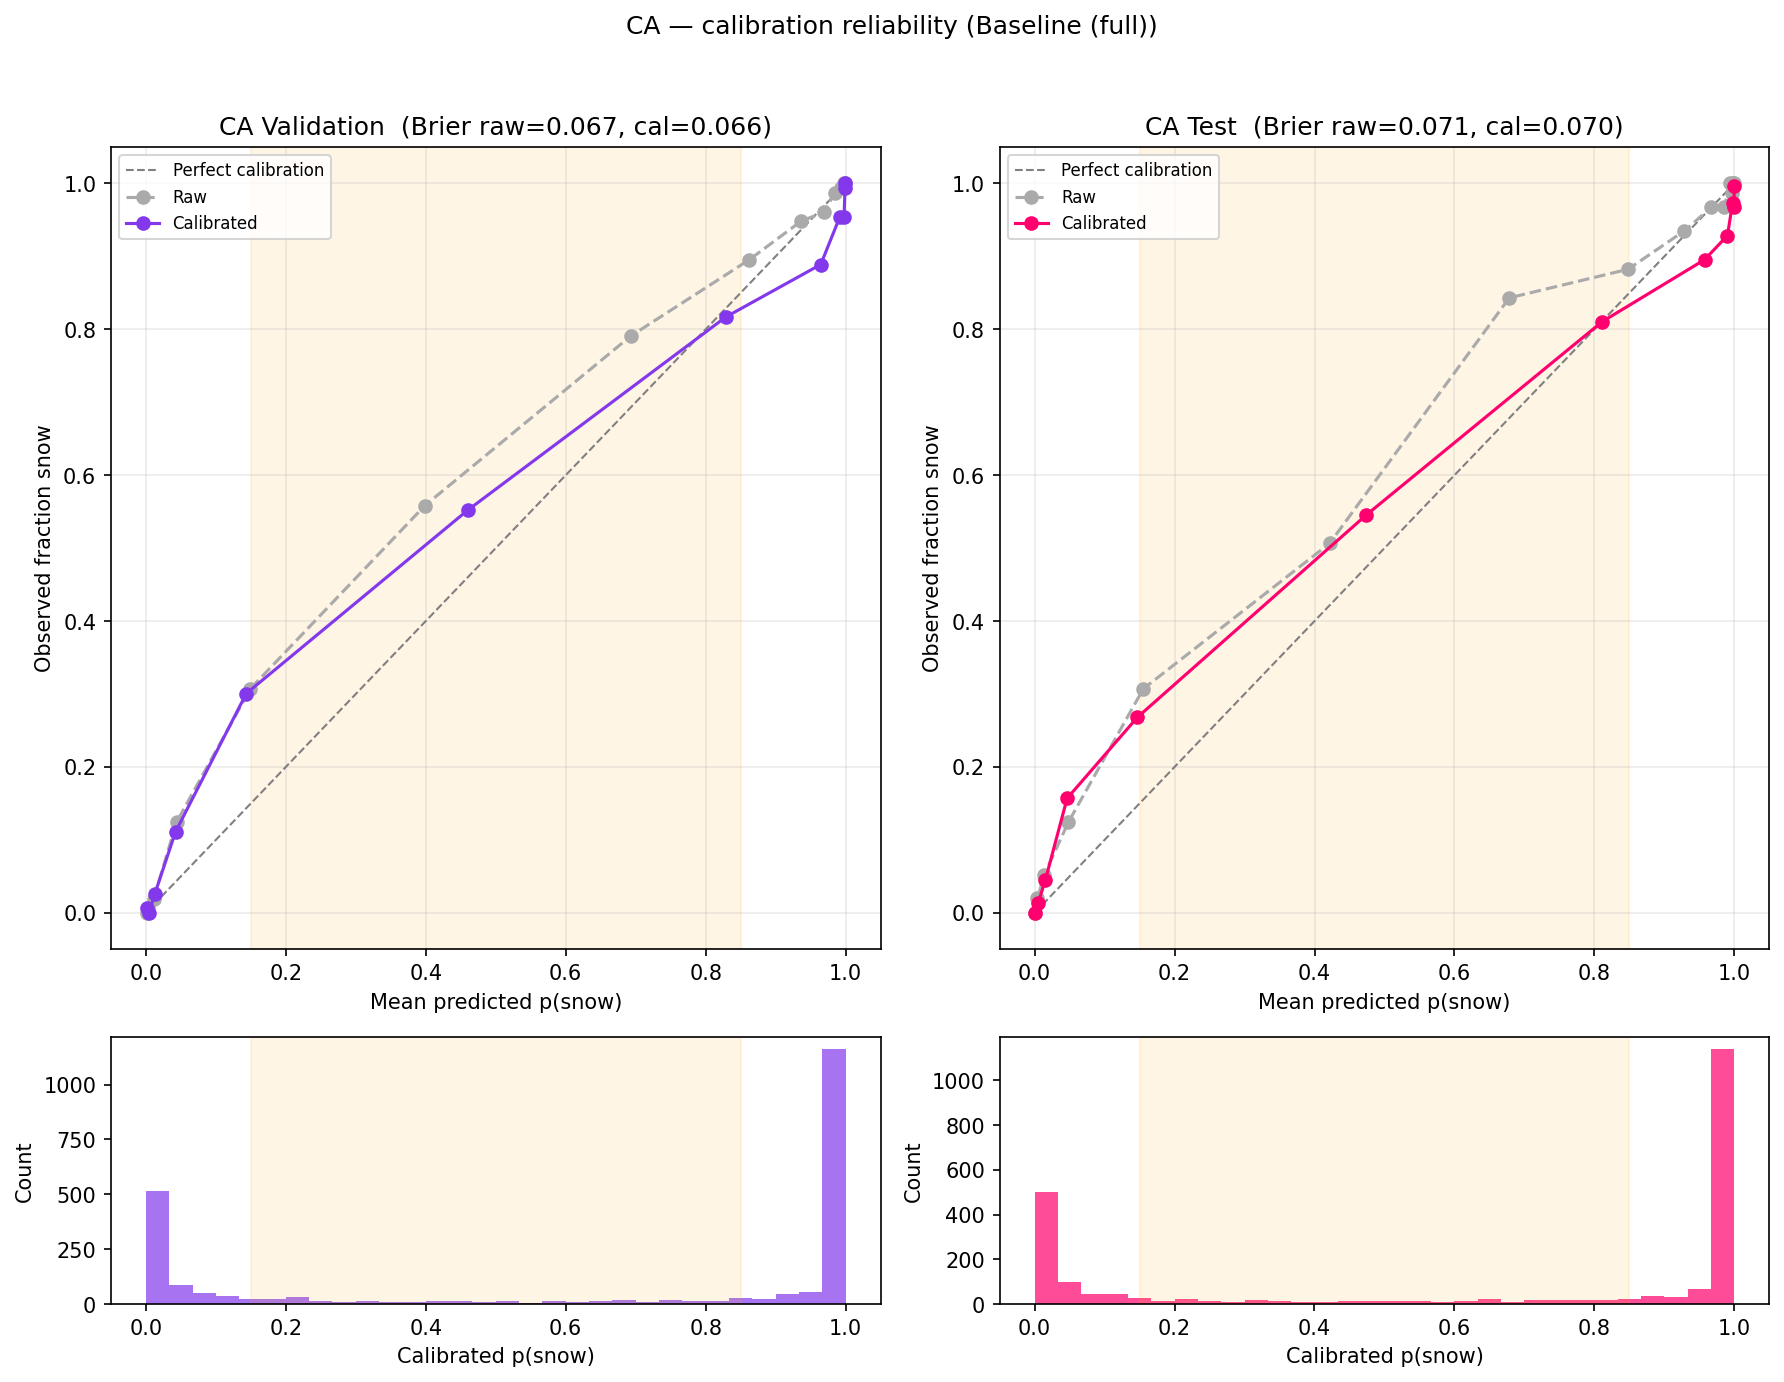
\includegraphics[width=0.49\textwidth]{CA/CA_calibration_reliability.png}
  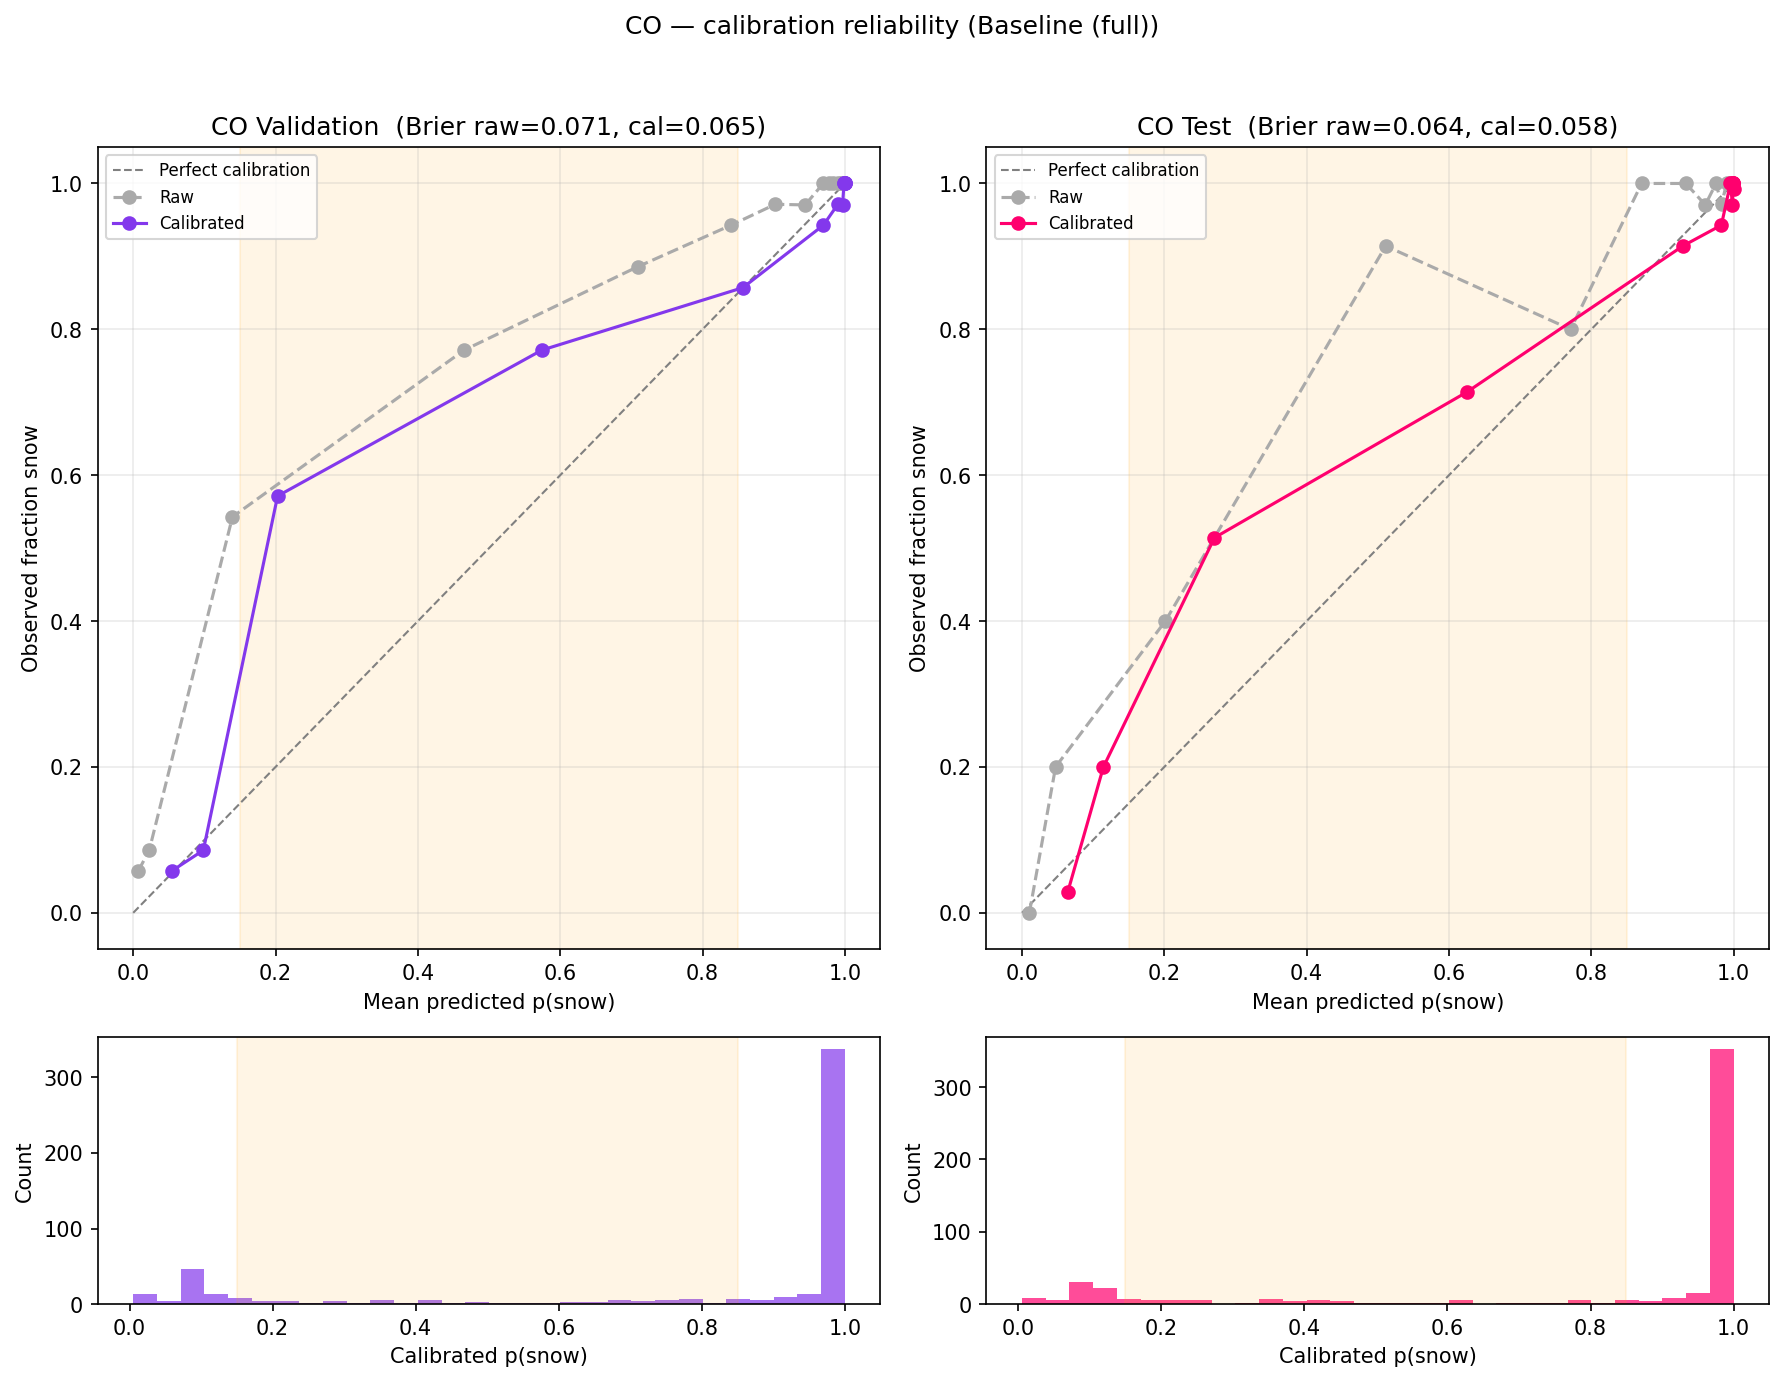
\includegraphics[width=0.49\textwidth]{CO/CO_calibration_reliability.png}
  \caption{Reliability diagrams and calibrated score distributions for
  California (left pair) and Colorado (right pair), validation and
  test. Beta calibration (colored) moves the raw XGBoost curve (gray)
  toward the diagonal; the shaded region marks the maximum extent of
  the uncertainty band at $T_w = \degC{0}$ (0.15--0.85). The bimodal
  score histograms show that most predictions are confident, with the
  band occupying the sparse middle.
  %
  Reliability curves use 15 quantile-spaced bins, so each point carries
  roughly equal sample weight and the visible spacing of points along the
  abscissa is itself informative: the wide gap across the middle of the
  range reflects how few predictions land there. Only pure snow and rain
  observations enter these diagrams, since calibration is defined
  against a binary outcome and observer-reported mix has no
  corresponding target probability; mix events are therefore absent here
  and assessed separately in Figure~\ref{fig:band}. Brier scores in the
  panel titles are computed on the same pure-phase subset, raw versus
  calibrated. Residual departures from the diagonal at the extreme bins
  should be read with the histogram beneath them, where the small
  denominators mean a handful of observations can move a bin's observed
  frequency substantially.}
  \label{fig:calibration}
\end{figure*}

\begin{figure*}[tp]
  \centering
  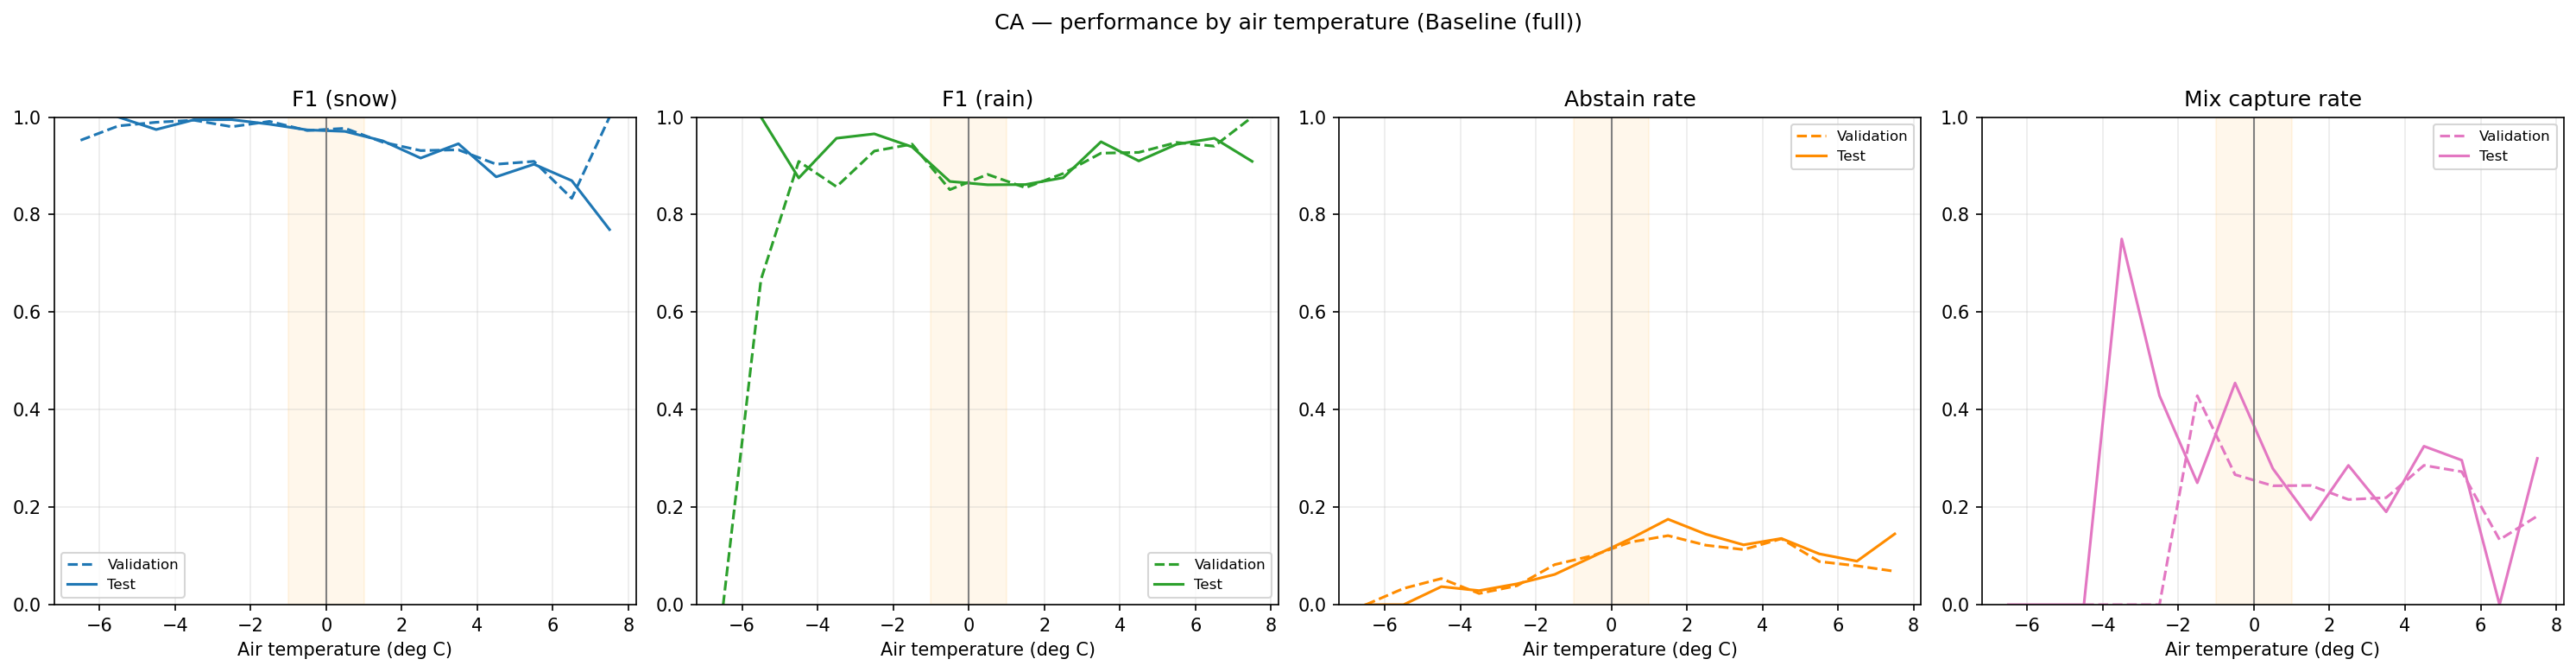
\includegraphics[width=0.95\textwidth]{CA/CA_f1_by_tair.png}\\[2pt]
  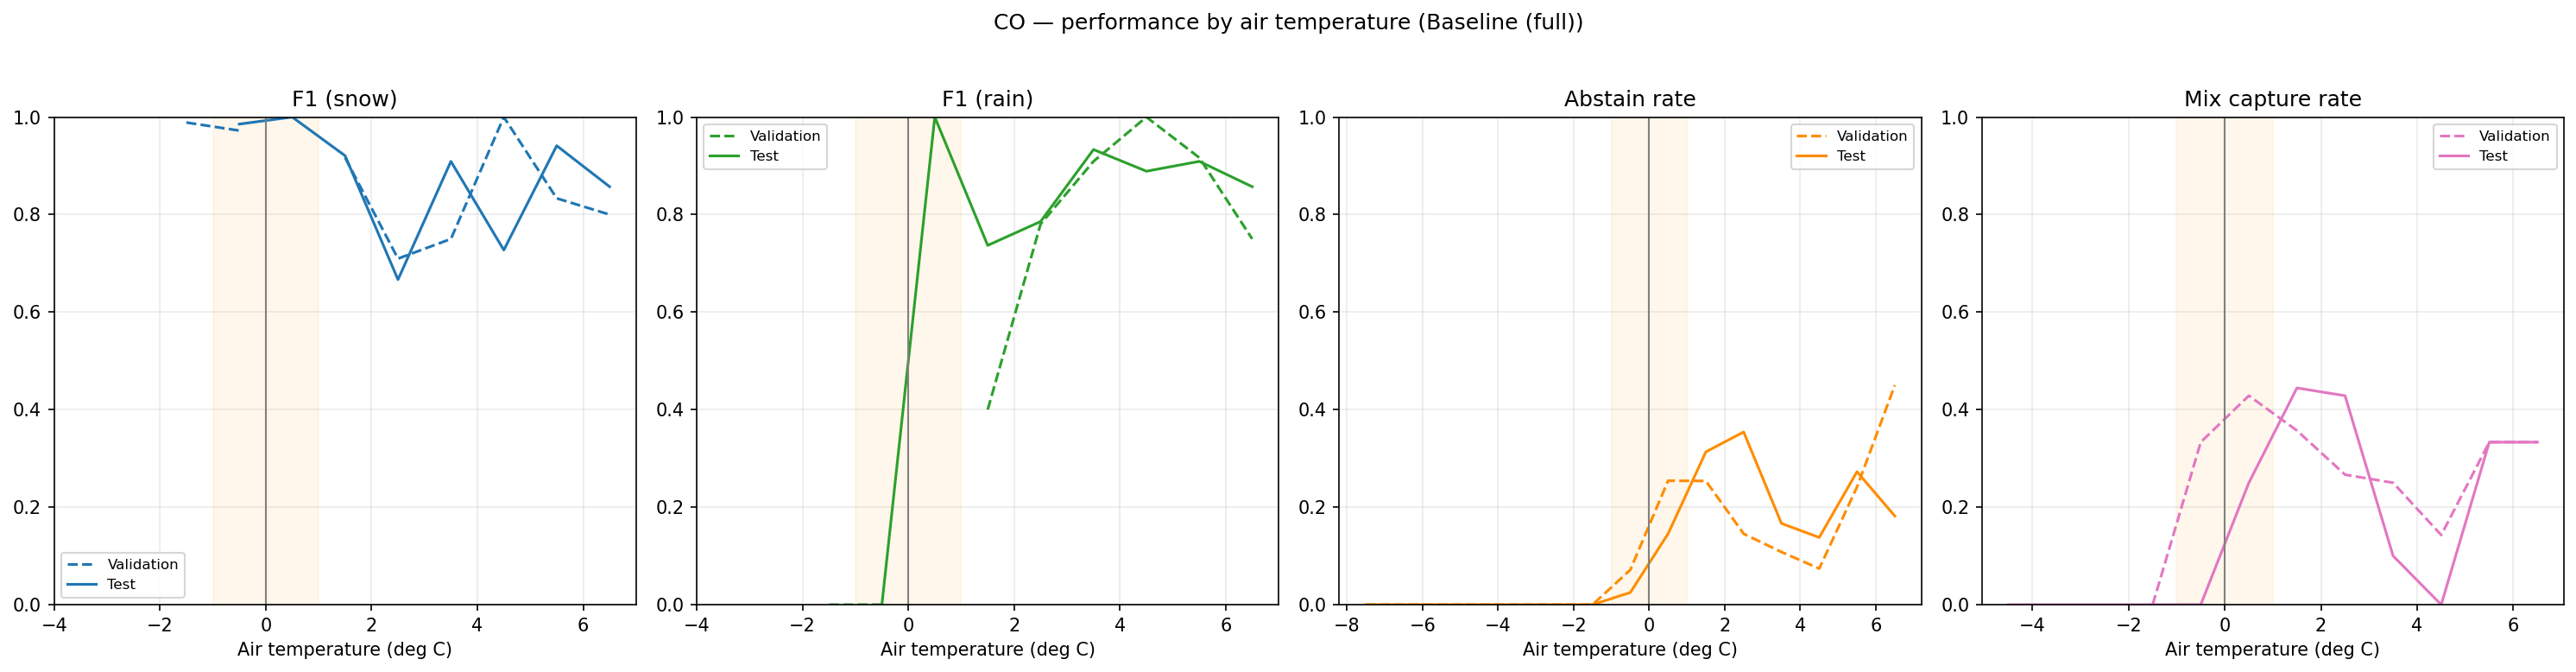
\includegraphics[width=0.95\textwidth]{CO/CO_f1_by_tair.png}
  \caption{Model performance in \degC{1} air-temperature bins for California (top)
  and Colorado (bottom), validation (dashed) and test (solid), with
  shading marking $\pm\degC{1}$ about freezing. Panels show snow F1, rain
  F1, the flag rate, and the mix-capture rate.
  %
  Two points follow. This is the air-temperature counterpart to the
  wet-bulb view of Figure~\ref{fig:twet} and reproduces the same
  structure, with snow F1 declining as temperature rises, rain F1
  improving, and the flag rate peaking just above \degC{0}, which
  confirms the envelope concentrates where phase is ambiguous under
  either temperature variable. And Colorado's curves are visibly noisier
  throughout, reflecting its smaller sample.
  %
  Conventions follow Figure~\ref{fig:twet}, except that bins span
  \degC{-8} to \degC{8} rather than \degC{-6} to \degC{6}, since air and
  wet-bulb temperature are physically distinct and reusing one set of
  edges would not be meaningful. F1 is computed only over committed
  observations, bins with fewer than 10 observations are dropped, and F1
  is undefined where a bin holds a single phase, which is what interrupts
  Colorado's curves below \degC{-2}. A plotted zero, as in Colorado's
  test rain F1 near \degC{-0.5}, instead means both phases were present
  and the model recovered no rain.}
  \label{fig:f1-temp}
\end{figure*}

\begin{figure*}[tp]
  \centering
  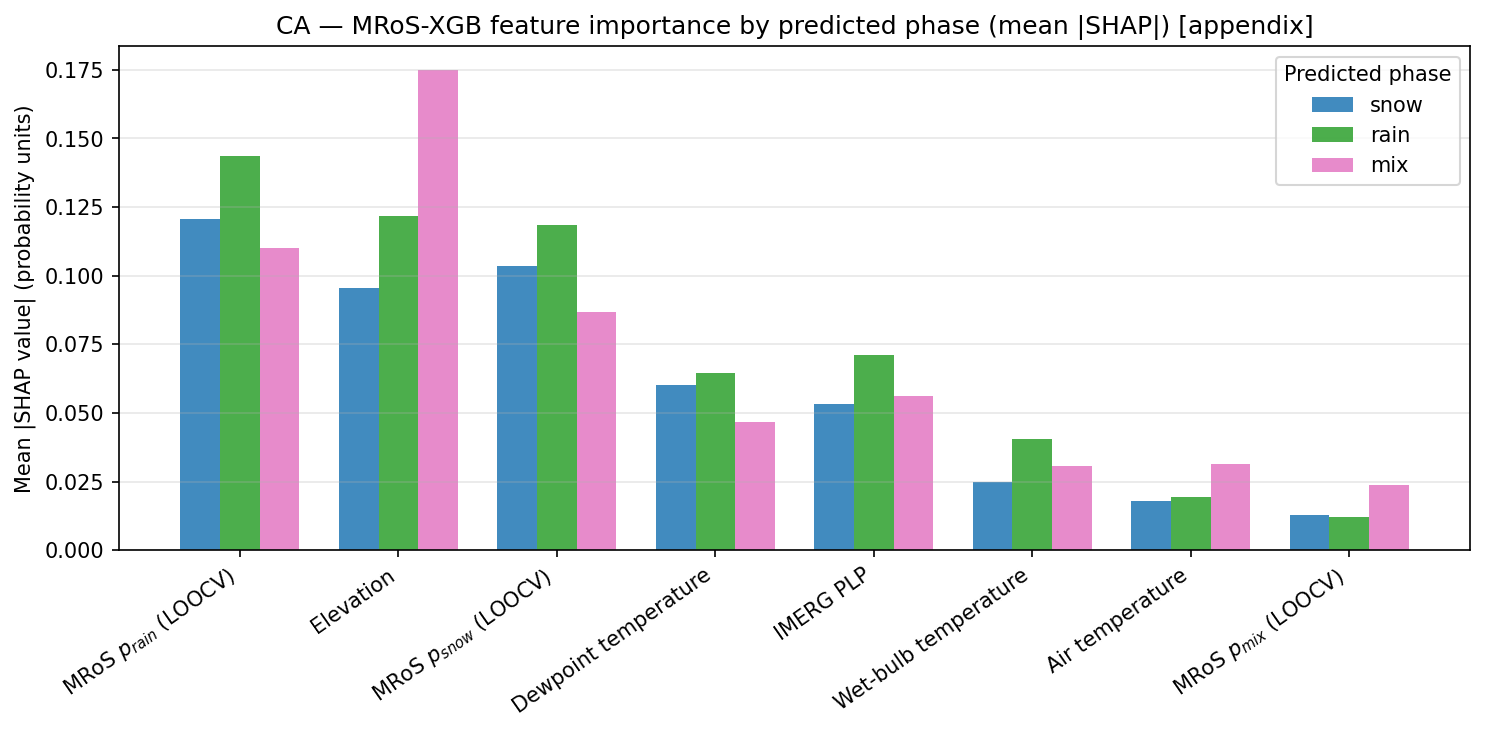
\includegraphics[width=0.95\textwidth]{CA/CA_shap_mean_by_phase_appendix.png}\\[2pt]
  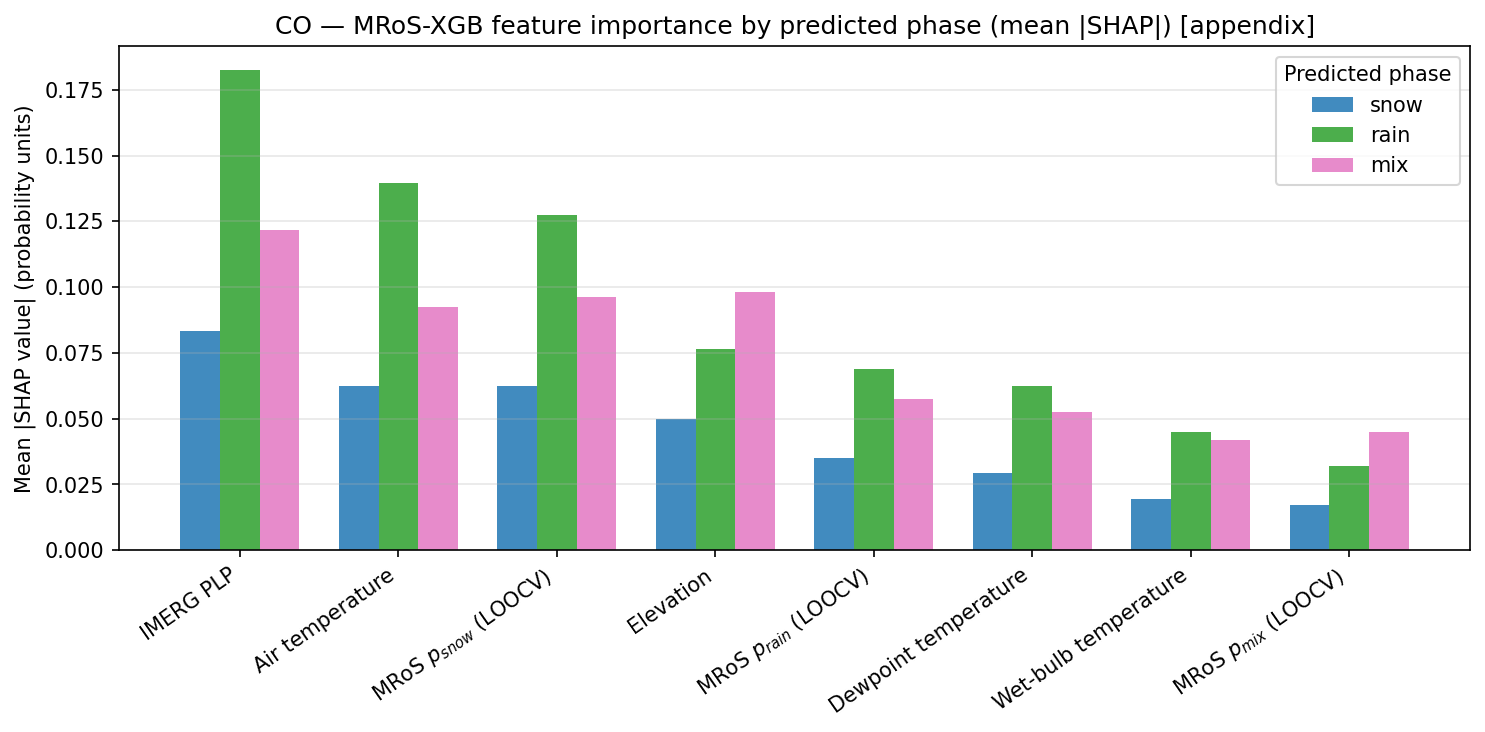
\includegraphics[width=0.95\textwidth]{CO/CO_shap_mean_by_phase_appendix.png}
  \caption{Mean absolute SHAP value per predictor, grouped by the phase the model
  predicted, for California (top) and Colorado (bottom). Bars are ordered
  by overall importance, in probability units, so a bar of 0.10 means the
  predictor moves $p(\mathrm{snow})$ by 0.10 on average. The domains rank
  their predictors differently: California leads with the crowdsourced
  surfaces and elevation, Colorado with IMERG pLP and air temperature.
  %
  Two features carry interpretive weight. Attributions are larger for
  rain and mix predictions than for snow in both domains, indicating the
  model needs more evidence to move away from the snow-dominant base rate
  than to stay with it. And correlation among predictors shapes these
  magnitudes: in California the MRoS snow and rain surfaces are
  anticorrelated at $r = -0.92$, air and wet-bulb temperature at $0.81$,
  and the MRoS snow surface with IMERG pLP at $-0.75$, so the crowdsourced
  surfaces are a spatial re-encoding of the thermodynamics rather than an
  independent signal, which is why credit transfers onto them and away
  from the raw temperatures.
  %
  Three limits apply to reading the bars. Groups are by \emph{predicted}
  phase, so ``mix'' is the set of predictions the band flagged rather than
  observed mix events. Mean absolute SHAP discards sign, so a large bar
  means strong response, not a push toward snow. And attributions are
  computed against each domain's own baseline, so bars compare within a
  panel but only loosely across domains.}
  \label{fig:app-shap}
\end{figure*}

\begin{figure*}[tp]
  \centering
  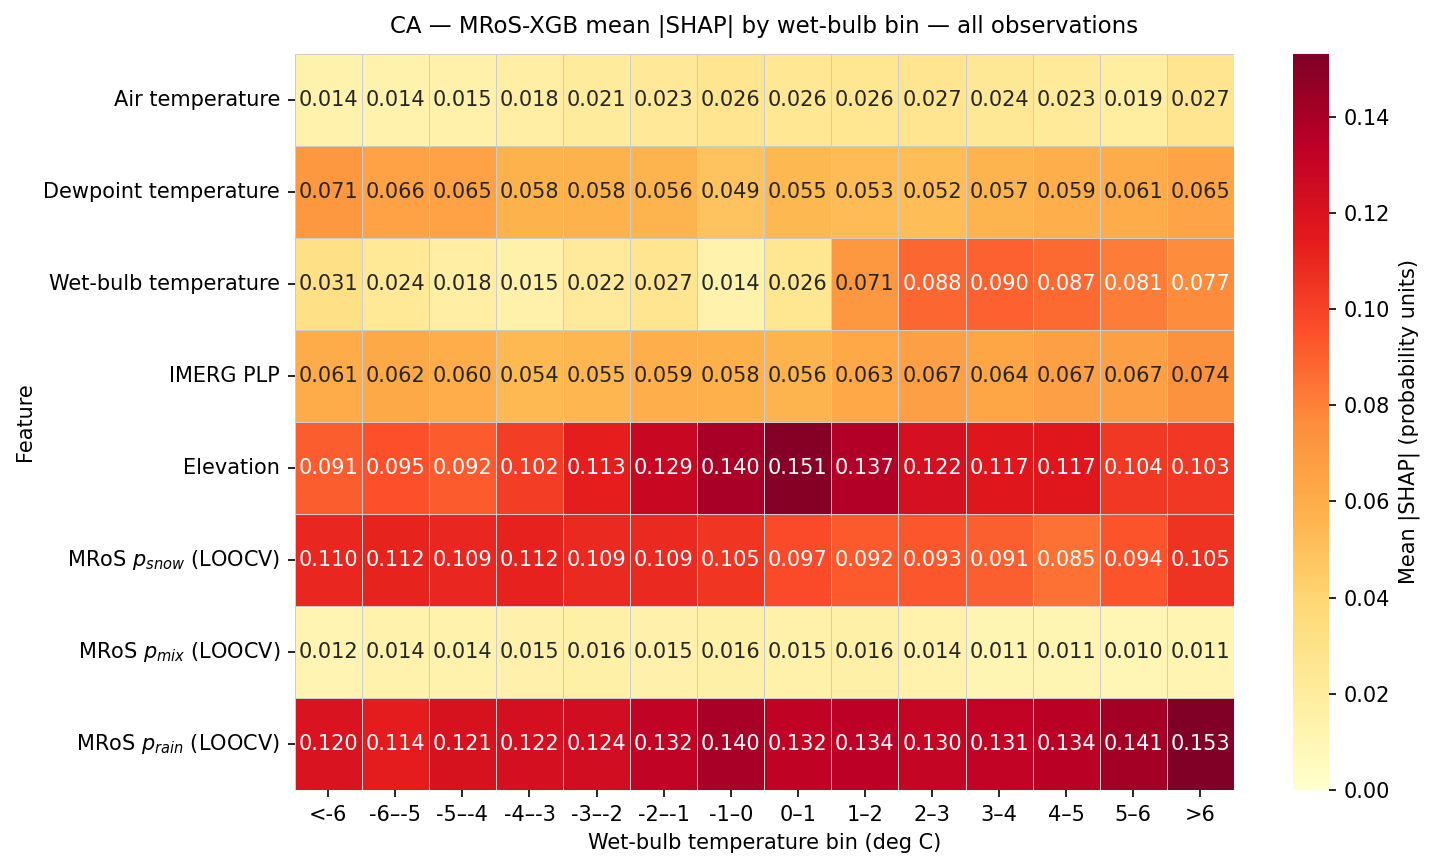
\includegraphics[width=0.95\textwidth]{CA/CA_shap_wetbulb_heatmap.png}\\[2pt]
  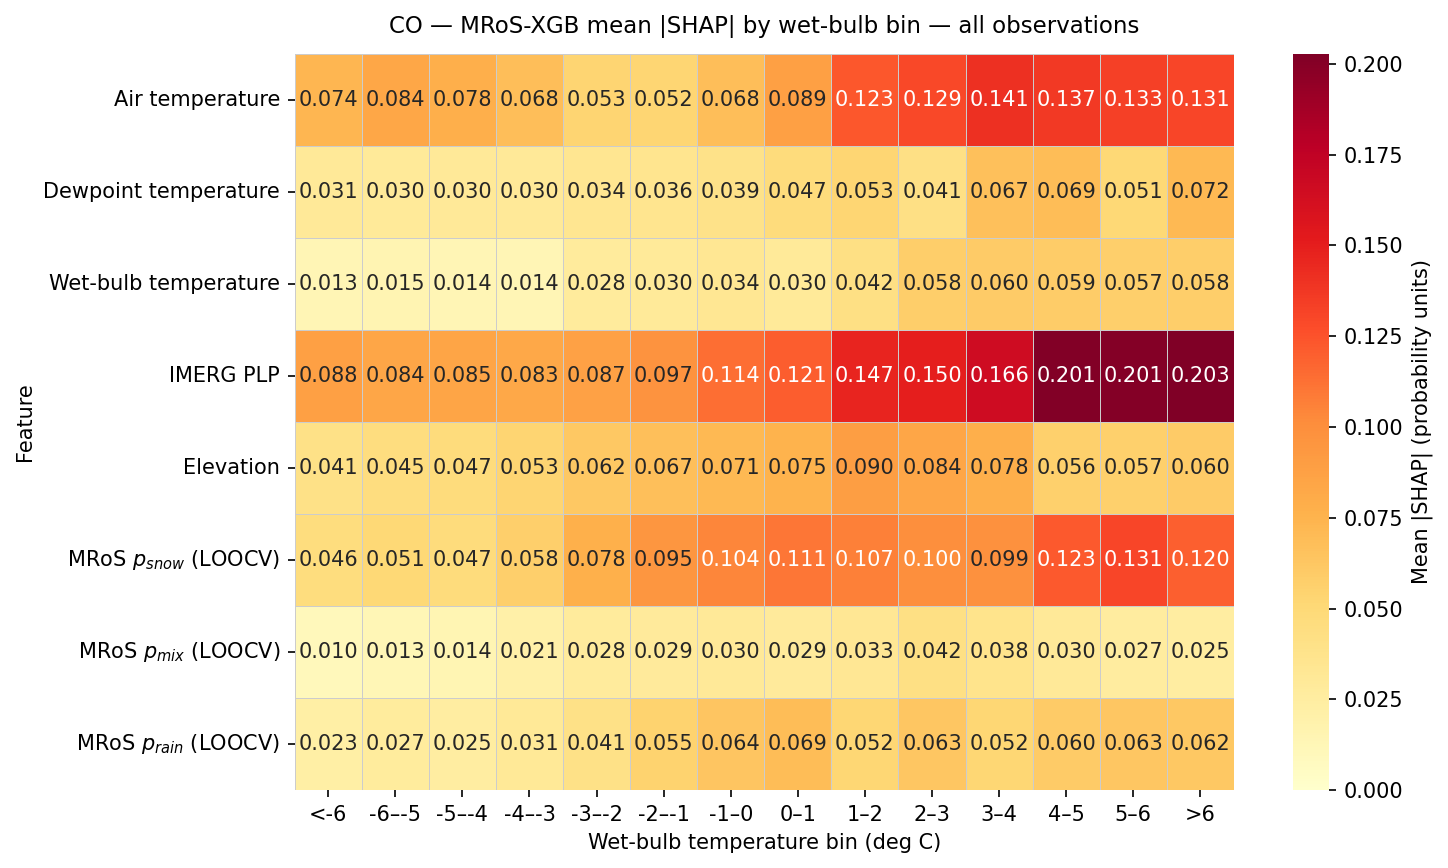
\includegraphics[width=0.95\textwidth]{CO/CO_shap_wetbulb_heatmap.png}
  \caption{Mean absolute SHAP value per predictor within \degC{1} wet-bulb bins,
  over all observations, for California (top) and Colorado (bottom).
  Whereas Figure~\ref{fig:app-shap} gives one number per predictor, this
  view resolves how the model reallocates reliance across the
  thermodynamic range.
  %
  Two contrasts matter. California's reliance on elevation peaks sharply
  in the transition zone (0.151 at $T_w$ = 0 to \degC{1}) while wet-bulb
  temperature contributes little below \degC{1} and rises several-fold
  once phase is unambiguous, whereas Colorado's reliance on IMERG pLP
  climbs monotonically from 0.088 in the coldest bin to 0.203 in the
  warmest. That is the attribution-side counterpart of the ablation
  result: California recruits terrain and the crowdsourced surfaces where
  the thermodynamic signal is weakest, while Colorado leans on the
  satellite column signal throughout. Summarized as a ratio of mean
  $|$SHAP$|$ near freezing to away from freezing, usage rises for air
  temperature ($1.44\times$), elevation ($1.38\times$), the MRoS mix
  surface ($1.14\times$) and rain surface ($1.10\times$), and falls for
  dewpoint ($0.84\times$).
  %
  Bin populations are strongly unequal, so a bright cell in an outer bin
  rests on far fewer observations than one near freezing, and empty bins
  are omitted rather than shown as zero. As in Figure~\ref{fig:app-shap}
  the quantity is unsigned, so these rows show where the model draws on a
  predictor, not which way it pushes the score.}
  \label{fig:shap-wetbulb}
\end{figure*}


% ======================================================================
\begin{figure*}[tp]
  \centering
  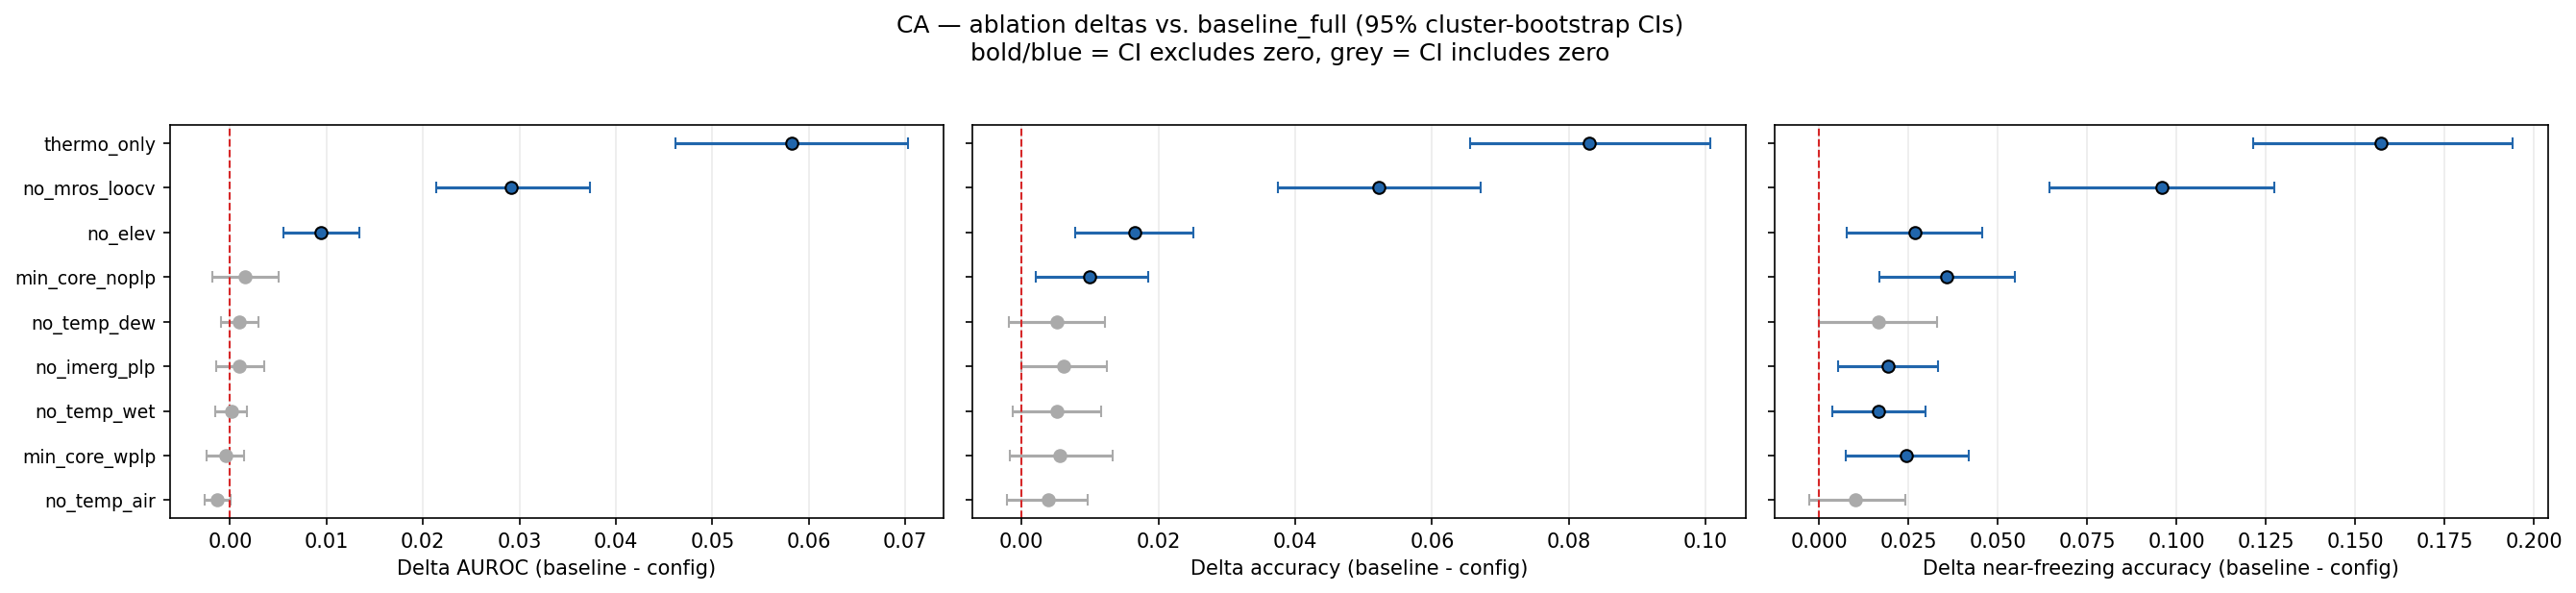
\includegraphics[width=0.95\textwidth]{CA/CA_ablation_deltas_ci.png}\\[2pt]
  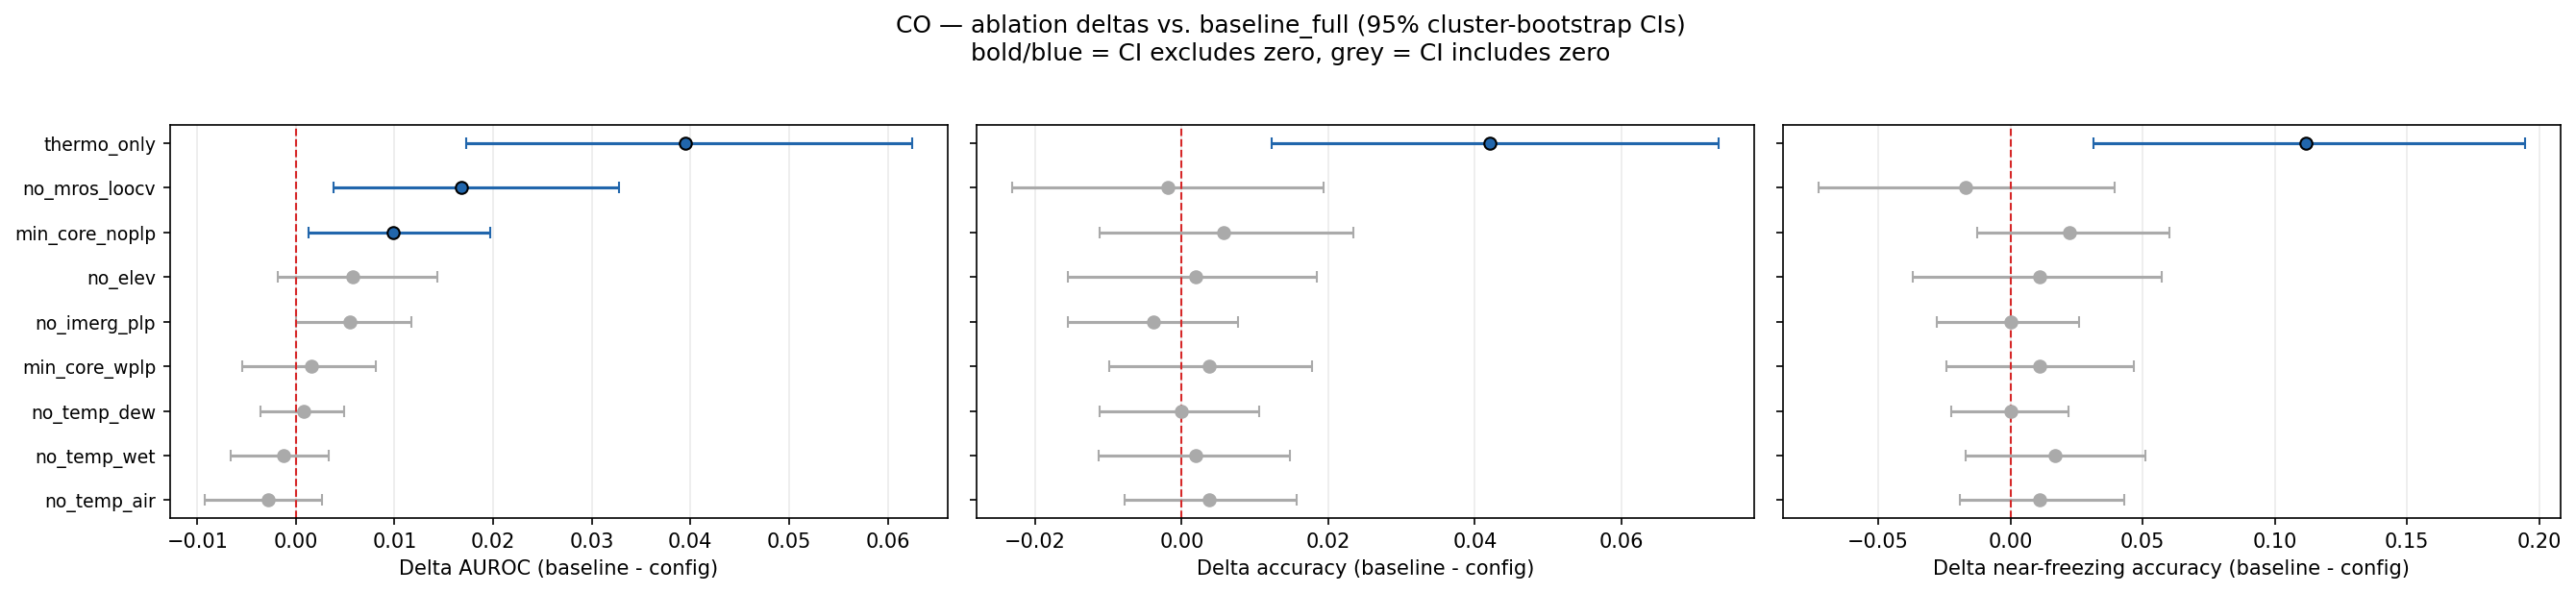
\includegraphics[width=0.95\textwidth]{CO/CO_ablation_deltas_ci.png}
  \caption{Ablation differences from the full model with 95\%
  cluster-bootstrap confidence intervals, for California (top) and
  Colorado (bottom): AUROC, overall accuracy, and near-freezing accuracy,
  each as baseline minus configuration, so positive values mean the
  removed predictors were contributing. Intervals are 2.5th--97.5th
  percentiles of 5{,}000 resamples over \mbox{30-km} $\times$
  calendar-day clusters, paired within resample; markers are drawn in
  blue with a dark edge where the interval lies clear of zero and grey
  where it crosses zero, and configurations are ordered by the difference in
  the leftmost panel so vertical position is comparable across panels.
  This is the interval-based counterpart to the point estimates
  underlying Table~\ref{tab:ablation}, and it is the version that
  supports the claims in Section~\ref{sec:ablation-results}: the
  thermodynamics-only configuration separates cleanly from the full model
  on every metric in both domains, whereas most single-predictor removals
  stay within noise, which is the signature of predictor redundancy rather
  than of predictors without value. Near-freezing accuracy carries wider
  intervals than overall accuracy throughout, since it is computed on the
  $|T_w| \le \degC{2}$ subset alone ($n = 782$ in California, $n = 179$
  in Colorado); differences that appear only there and not in the overall
  metric should be read as suggestive. No macro-F1 difference was
  archived in the bootstrap output, so that metric appears in
  Table~\ref{tab:ablation} but not here.}
  \label{fig:ablation-ci}
\end{figure*}

\begin{figure*}[tp]
  \centering
  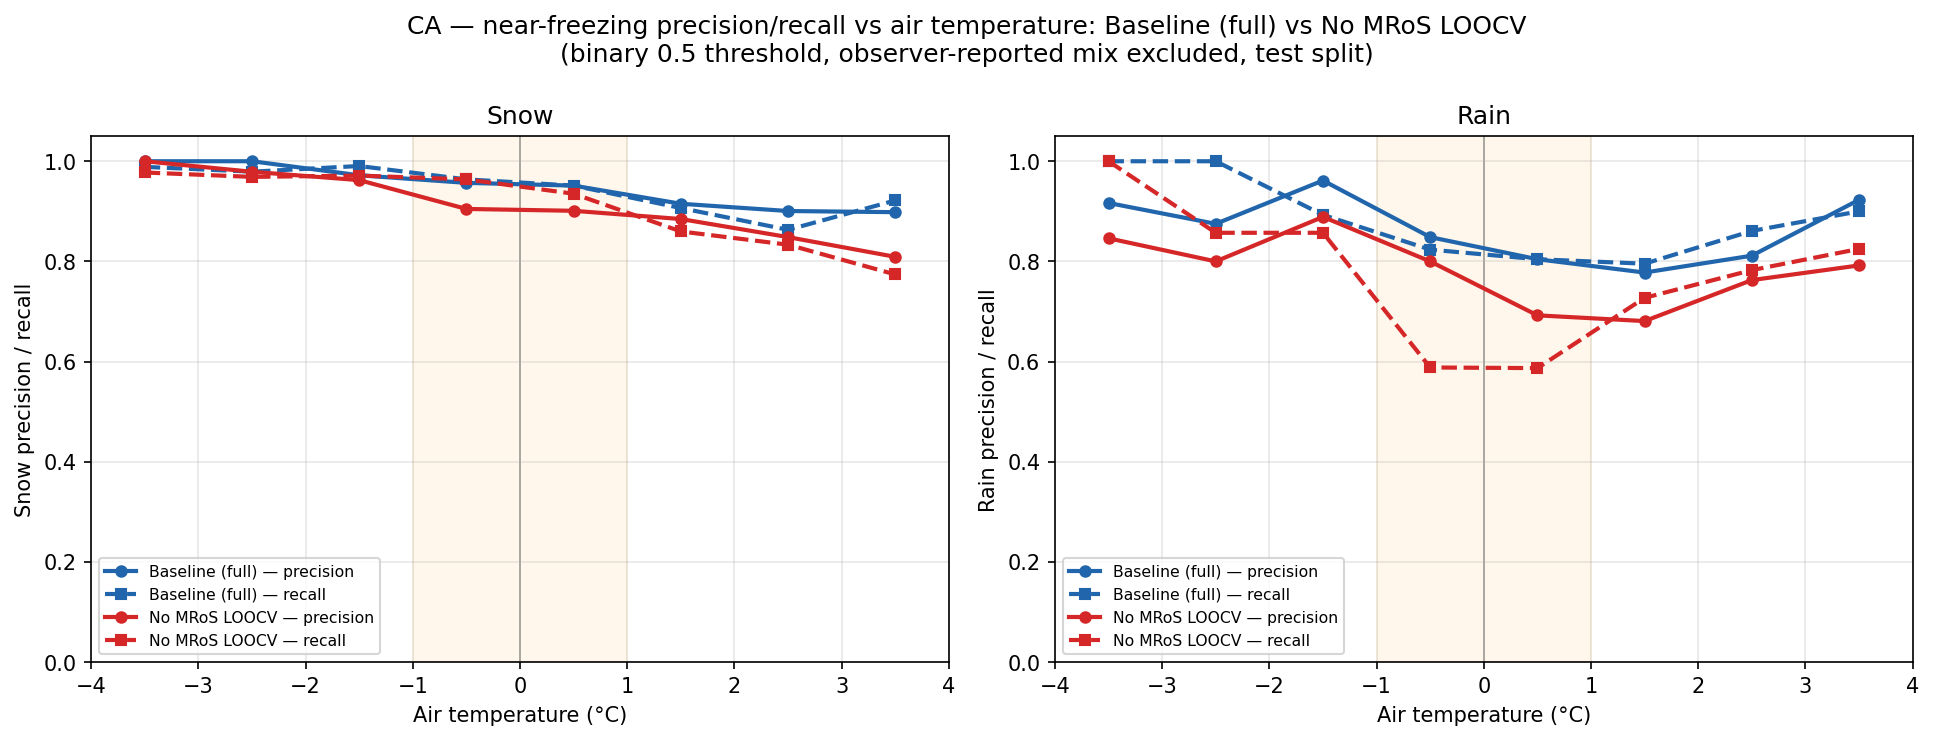
\includegraphics[width=0.95\textwidth]{CA/CA_story5_nearfreeze_tair_comparison.png}\\[2pt]
  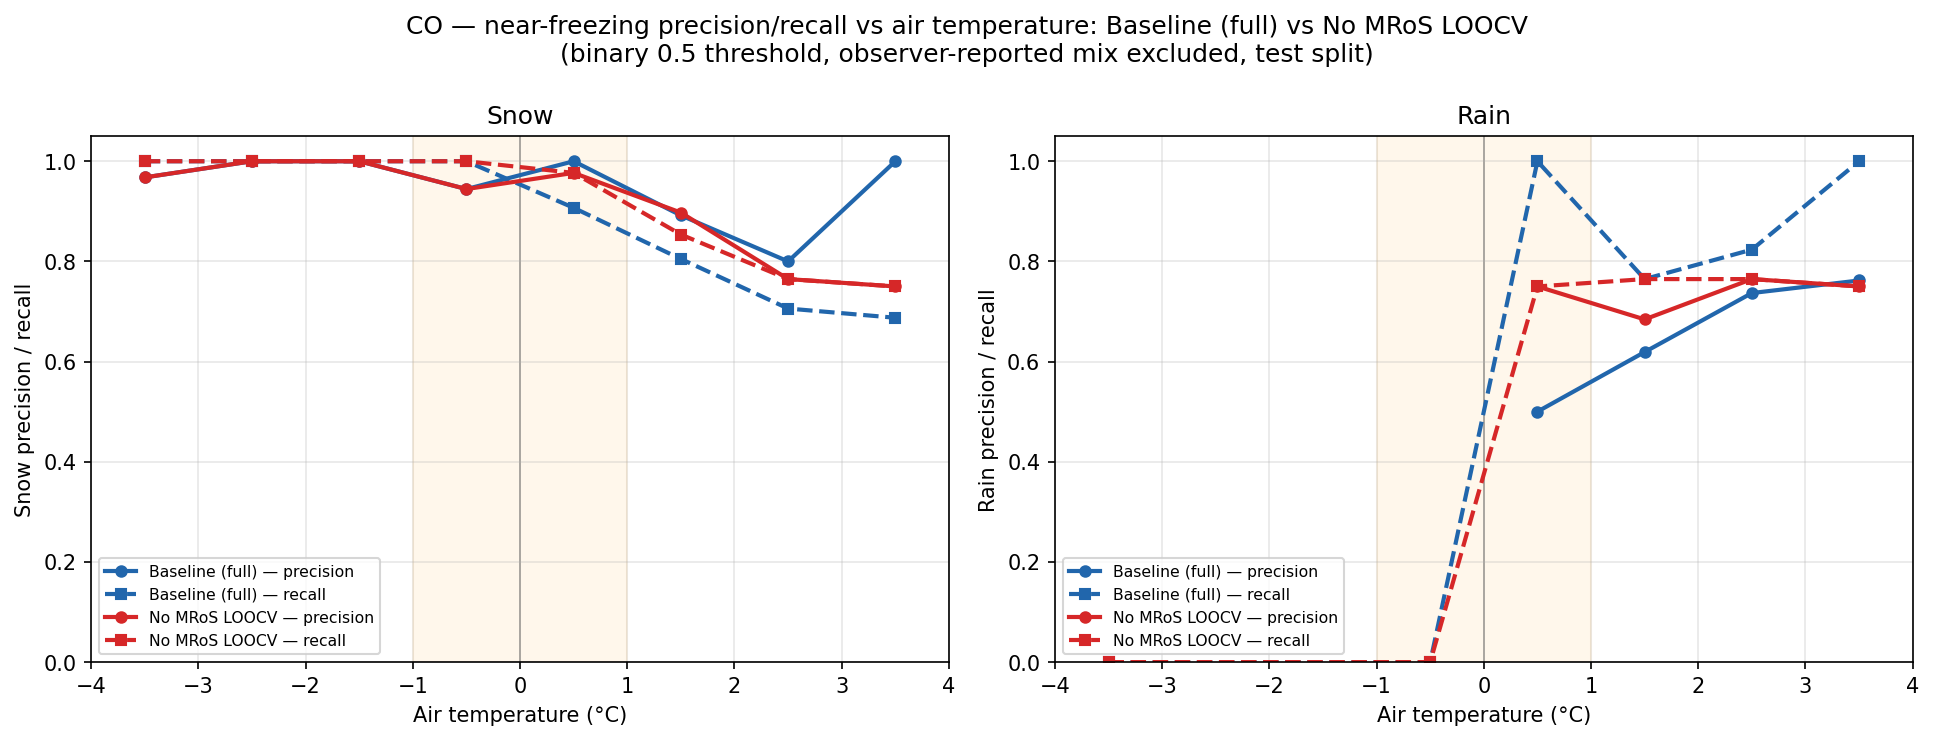
\includegraphics[width=0.95\textwidth]{CO/CO_story5_nearfreeze_tair_comparison.png}
  \caption{Air-temperature counterpart to
  Figure~\ref{fig:mros-contrib}: near-freezing precision and recall for
  the full model versus the model without the MRoS LOOCV surfaces, in
  \degC{1} air-temperature bins on the held-out test split, scored at the
  raw $0.5$ threshold with mix excluded. Binning against air temperature
  relocates the effect rather than removing it. In California the loss
  now appears in rain recall instead of snow recall --- $0.82$ falling to
  $0.59$ at \degC{-0.5} and $0.80$ to $0.59$ at \degC{0.5} --- because
  air temperature discriminates phase less sharply than wet-bulb
  temperature, so the bins mix thermodynamic regimes that the wet-bulb
  view separates. That the attributable loss survives the change of
  binning variable, while moving between phases, is the robustness point:
  the crowdsourced surfaces are supplying information the temperature
  fields do not carry, not sharpening a particular temperature
  threshold. Colorado's rain curves are undefined or near-degenerate in
  several cold bins here, where its rain sample is only a handful of
  observations, and should not be interpreted.}
  \label{fig:mros-contrib-tair}
\end{figure*}

\begin{figure*}[tp]
  \centering
  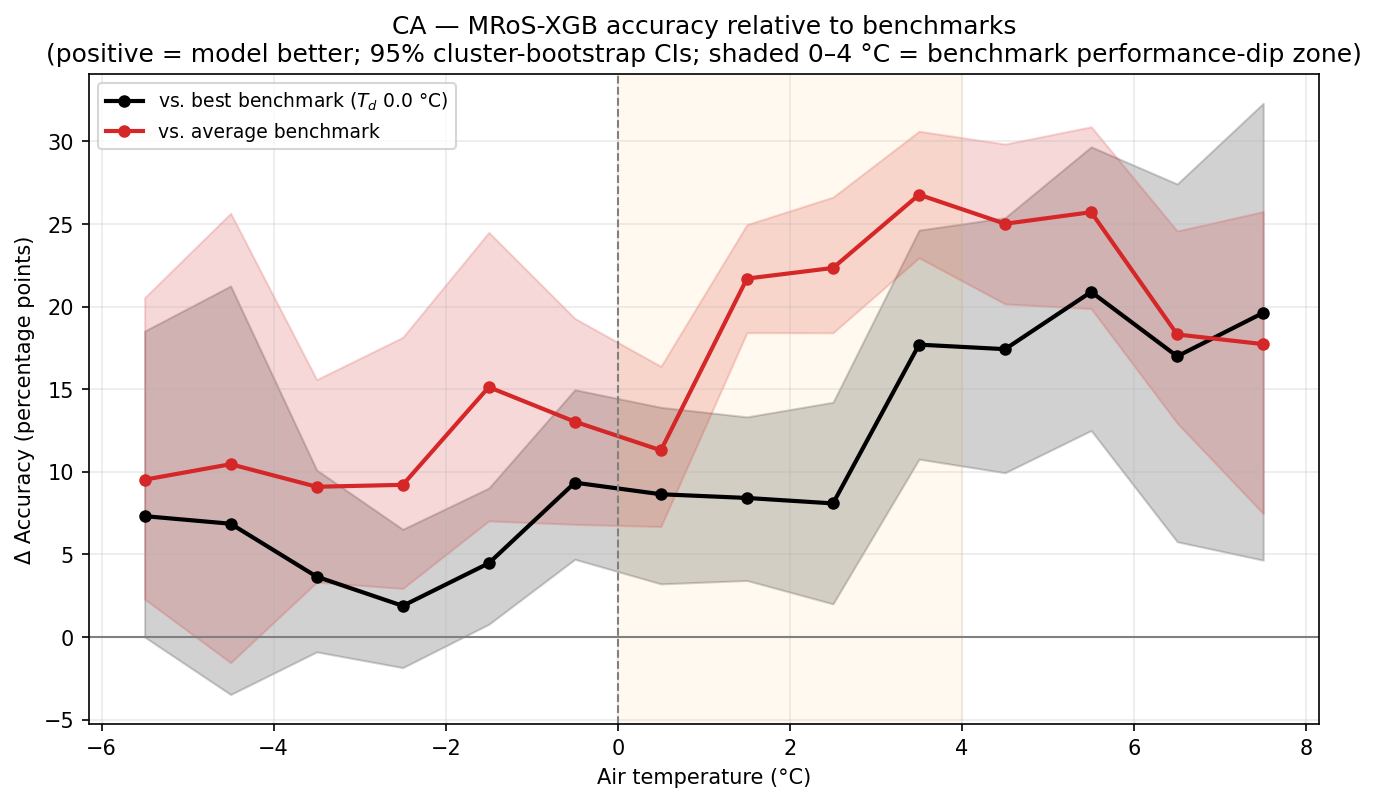
\includegraphics[width=0.47\textwidth]{CA/CA_benchmark_relative_improvement_ci.png}
  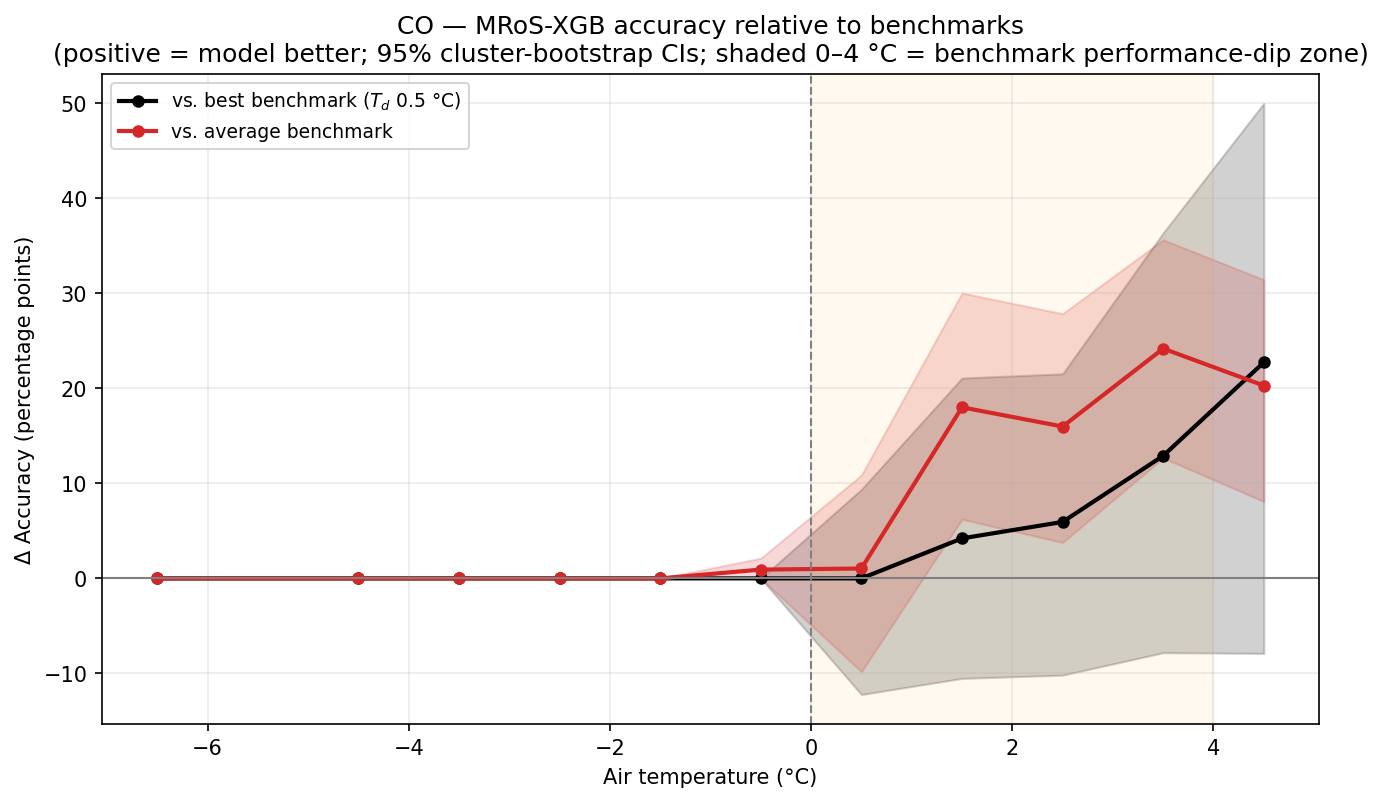
\includegraphics[width=0.47\textwidth]{CO/CO_benchmark_relative_improvement_ci.png}
  \caption{Model accuracy relative to the benchmarks by air-temperature
  bin, California (left) and Colorado (right): percentage-point
  difference against the best single benchmark (black) and against the
  mean of all nine (red), with 95\% cluster-bootstrap ribbons, positive
  meaning the model is more accurate. This is the difference form of
  Figure~\ref{fig:tair}, and it states the paper's central benchmark
  claim compactly: the advantage is smallest in the cold bins, where
  every method gets phase right, and rises into the shaded
  \degC{0}--\degC{4} zone where thresholds fail, reaching roughly 18
  percentage points against the best benchmark and 27 against the
  benchmark average in California. Two cautions. Differences are paired
  within each resample, so the ribbons describe uncertainty in the
  difference rather than in either accuracy separately, and the
  vs.\ average-benchmark line is not a comparison against any deployable
  method --- it summarizes the family and is the more favorable of the
  two framings. The cold-bin ribbons cross zero in both domains, so we do
  not claim an advantage there; the claim is specifically about the
  transition zone.}
  \label{fig:relimp}
\end{figure*}

\begin{figure*}[tp]
  \centering
  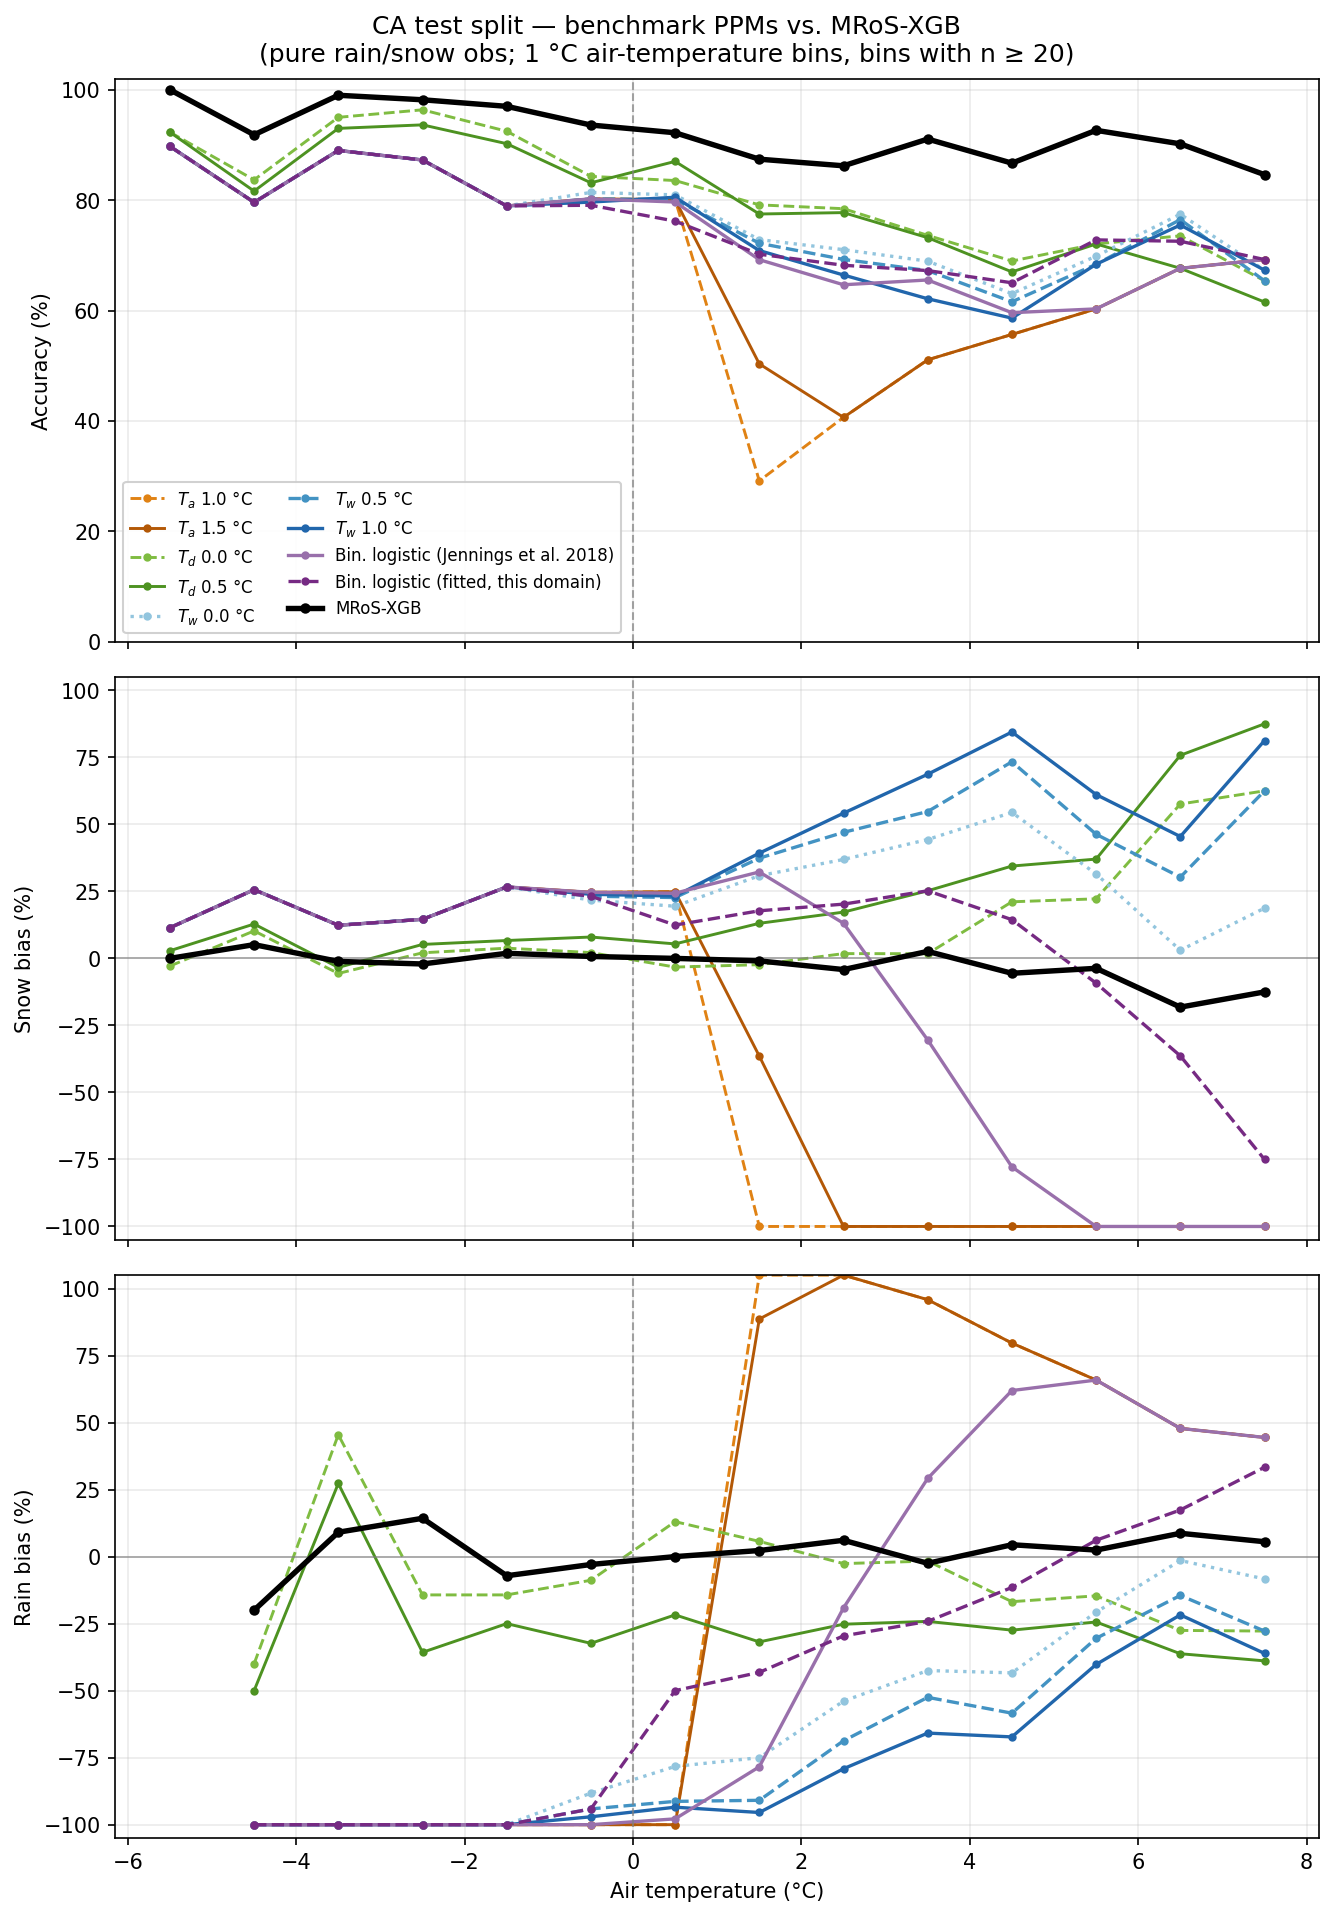
\includegraphics[width=0.47\textwidth]{CA/CA_benchmark_accuracy_by_tair.png}
  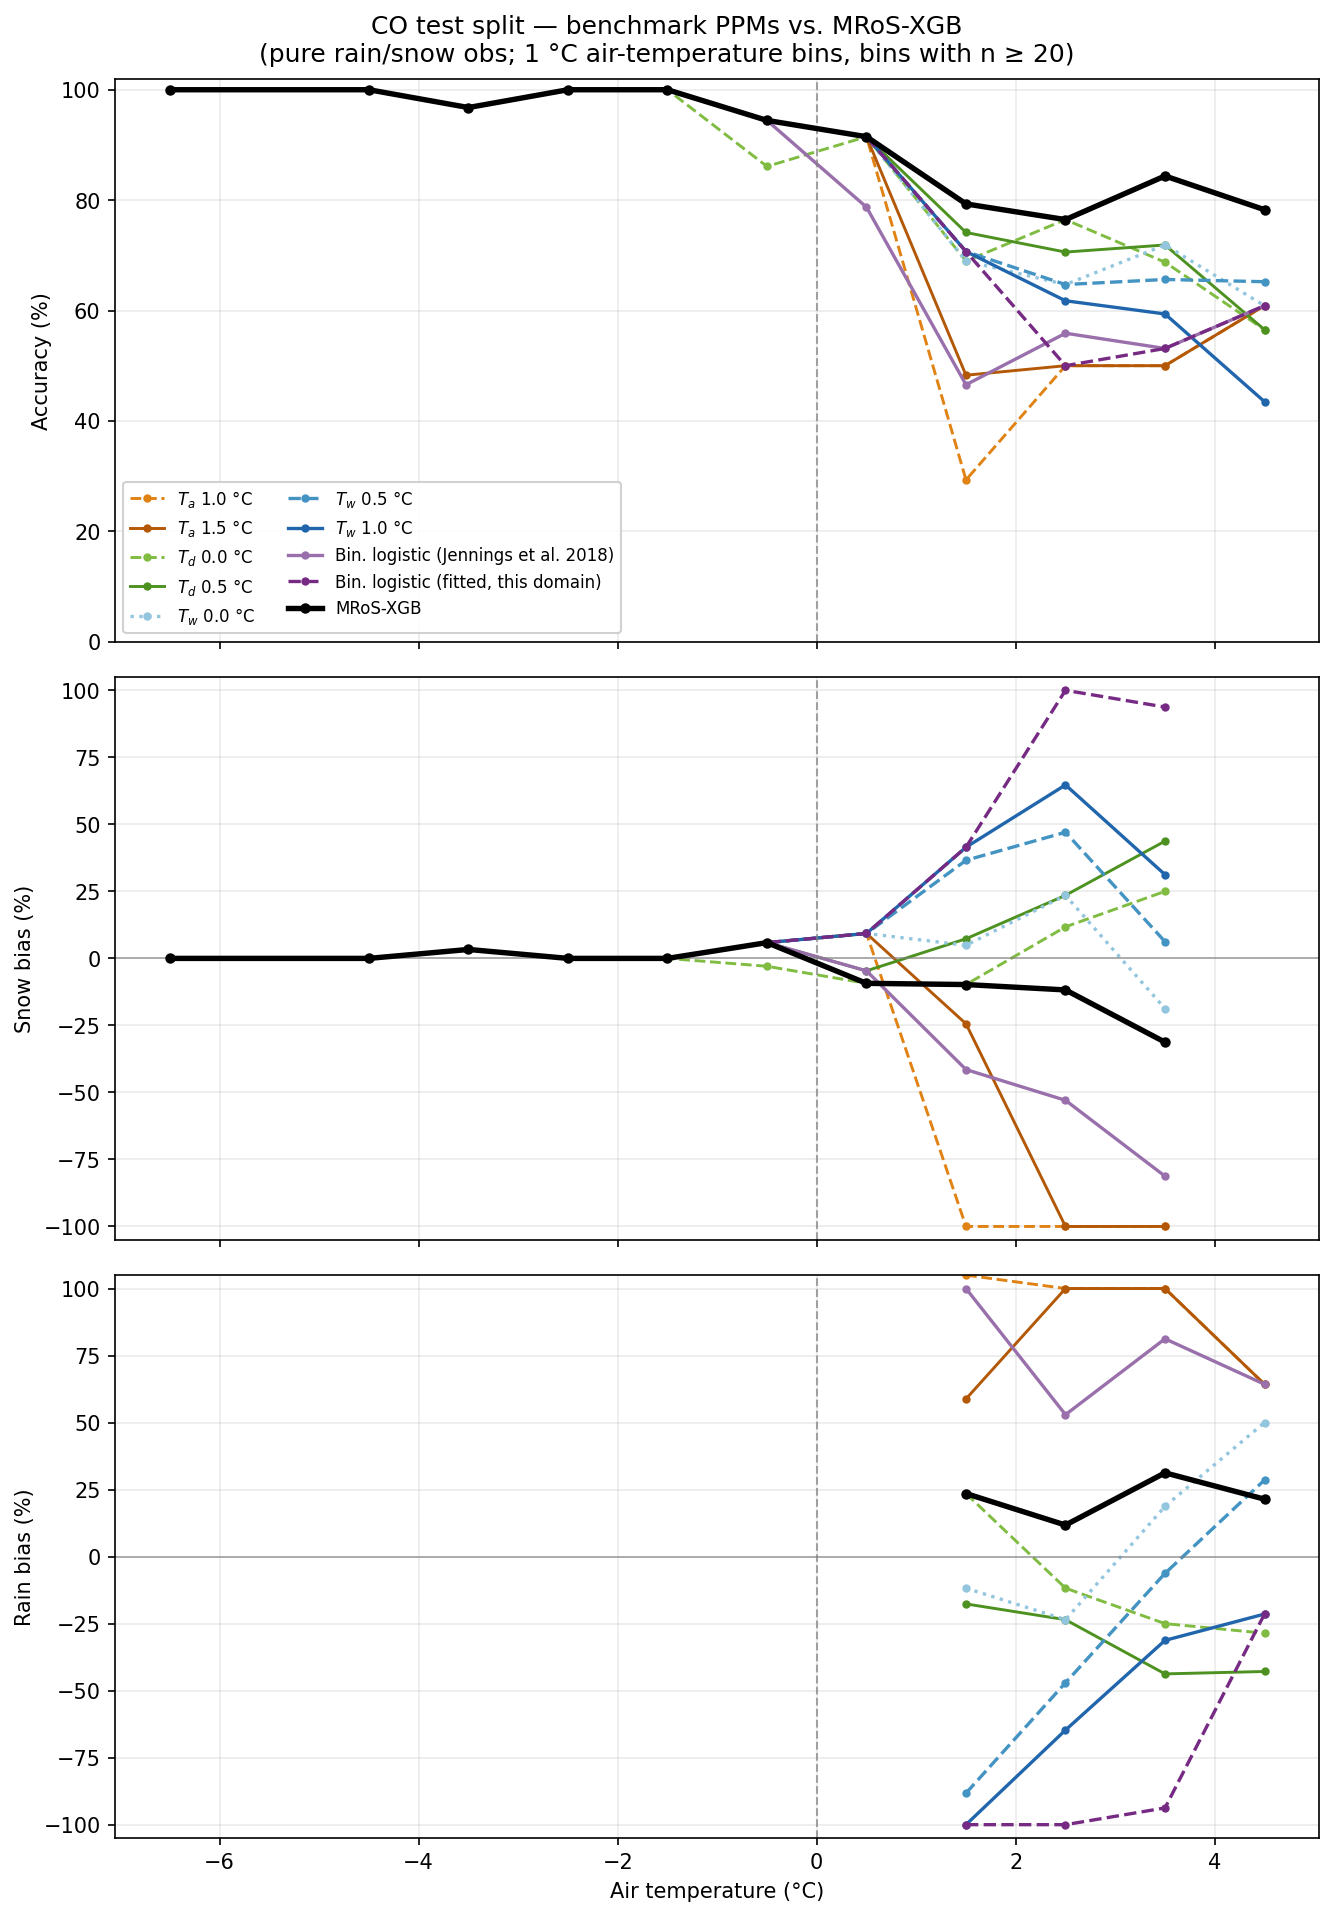
\includegraphics[width=0.47\textwidth]{CO/CO_benchmark_accuracy_by_tair.png}
  \caption{Accuracy and per-phase bias against air temperature for all
  nine benchmark partitioning methods and the model, California (left)
  and Colorado (right), held-out test split, \degC{1} bins with $n \ge
  20$ pure observations. Panels give, from top to bottom, accuracy, snow
  bias, and rain bias, where bias is the signed difference between
  predicted and observed frequency of that phase within the bin, so zero
  is unbiased and positive means over-prediction. These are point
  estimates without intervals; Figure~\ref{fig:tair} gives the
  bootstrap-resampled version for the model and best benchmark.
  The bias panels are the reason to include this figure: they show
  \emph{how} fixed-threshold methods fail rather than only that they do.
  Each threshold method's error is a compensating pair --- systematic
  snow over-prediction on the warm side of its threshold and rain
  over-prediction on the cold side --- so its accuracy in any single bin
  understates the structure of the error, and bins where two methods tie
  on accuracy can be biased in opposite directions. The model's bias
  curves stay closer to zero across the range rather than trading one
  phase against the other, which is what a threshold-free partition
  should look like. Colder and warmer bins are dropped where fewer than
  20 pure observations are available, so the curves do not all span the
  same range.}
  \label{fig:tair-bias}
\end{figure*}


\begin{figure*}[tp]
  \centering
  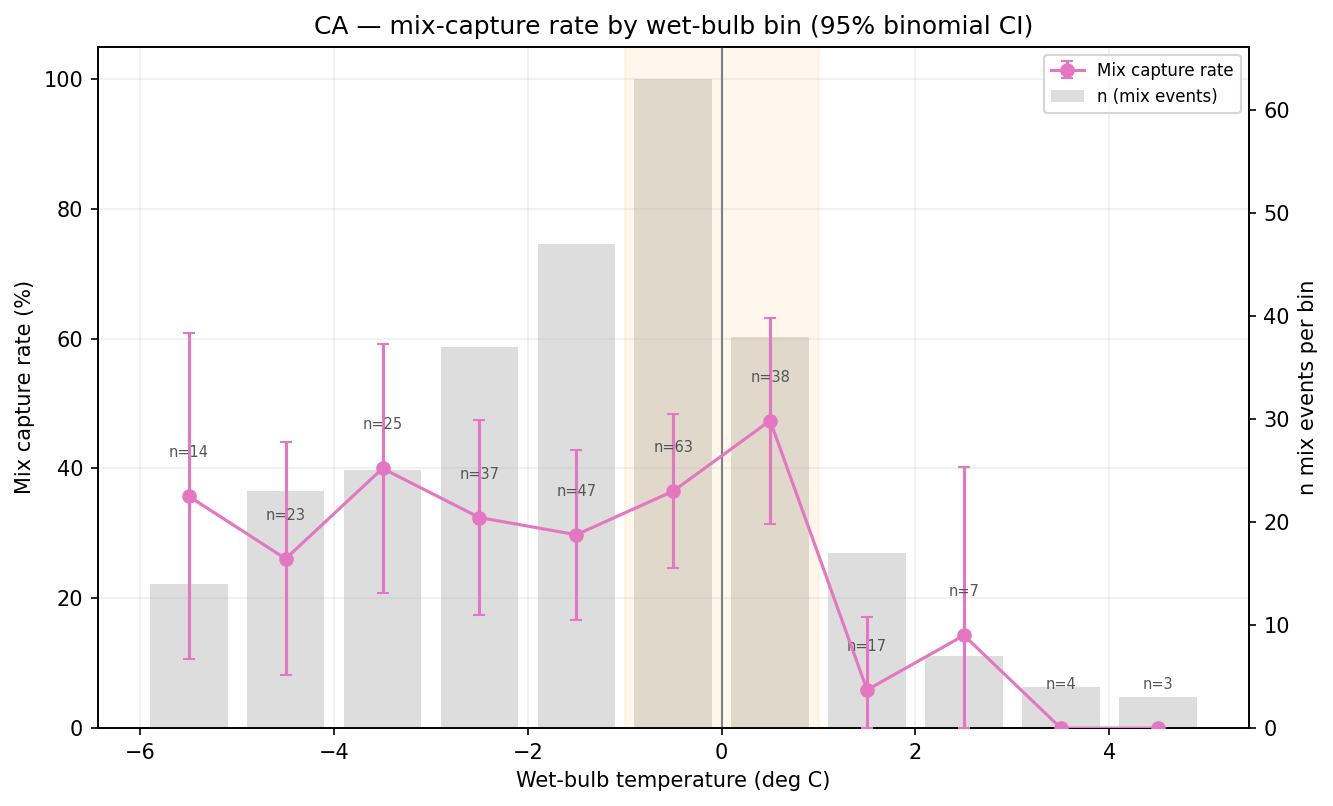
\includegraphics[width=0.95\textwidth]{CA/CA_mix_capture_by_wetbulb.png}\\[2pt]
  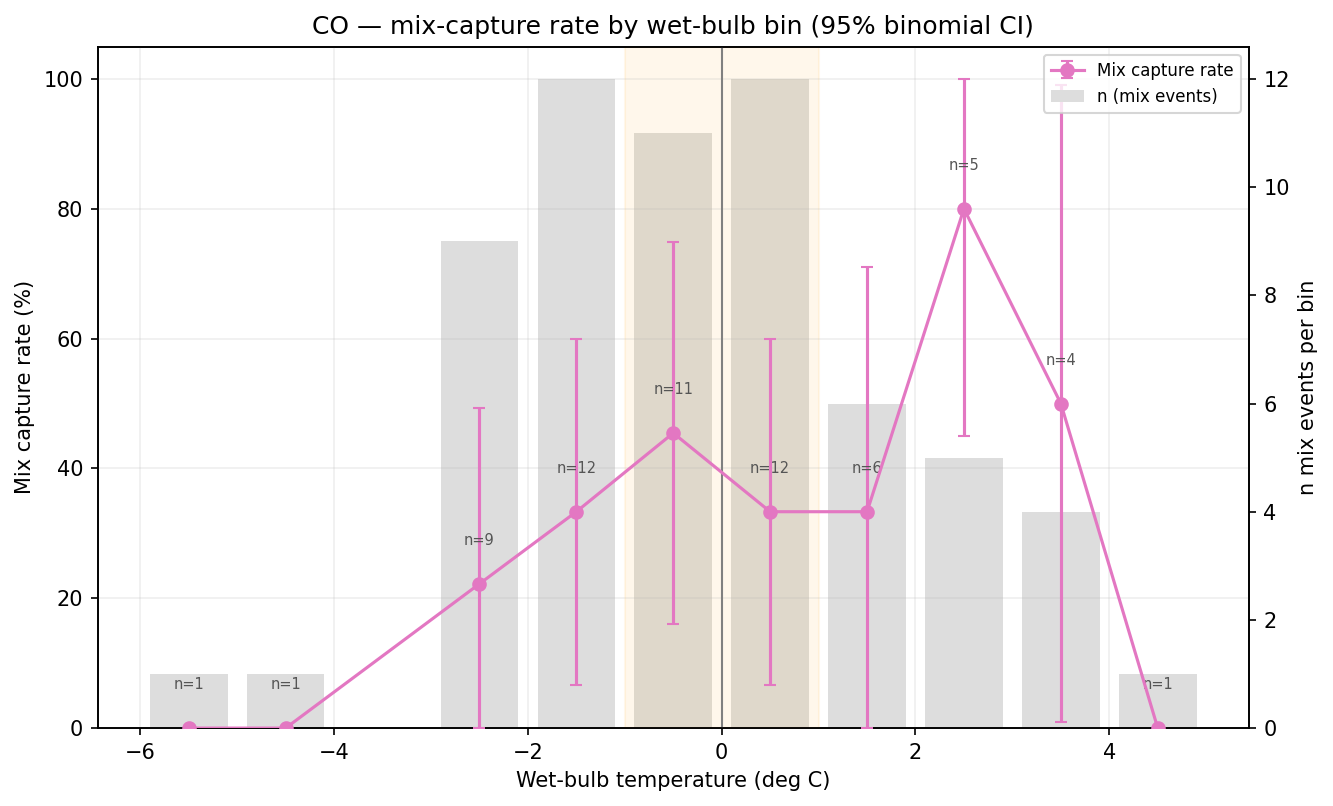
\includegraphics[width=0.95\textwidth]{CO/CO_mix_capture_by_wetbulb.png}
  \caption{Mix-capture rate by \degC{1} wet-bulb bin for California (top) and
  Colorado (bottom), held-out test split. Points give the fraction of
  observer-reported mix events per bin whose calibrated
  $p(\mathrm{snow})$ falls inside the uncertainty band, with 95\%
  intervals; grey bars give the mix-event count per bin on the
  right-hand axis, and shading marks $|T_w| \le \degC{1}$.
  %
  Two results stand out. Capture is highest in the near-freezing bins
  where mixed precipitation actually occurs ($47\%$ at
  $T_w = \degC{0.5}$ in California) and falls away on either side, which
  is the intended behavior, since the band is placed to flag ambiguity
  rather than to maximize capture everywhere. And pooled capture, $31\%$
  in California and $36\%$ in Colorado, agrees with the independent
  test-set bootstrap estimates of $0.30$ and $0.33$ in
  Table~\ref{tab:bootstrap}.
  %
  Interval construction differs from every other estimate in this paper.
  The saved prediction file for this diagnostic carries no cluster key, so
  the intervals shown are simple per-bin binomial intervals that treat mix
  events as independent. Because nearby simultaneous reports are not
  independent, these are optimistic, and the pooled figures in
  Table~\ref{tab:bootstrap} are the ones to quote. Several tail bins rest
  on fewer than ten events, where a rate of $0\%$ or $100\%$ reflects a
  handful of observations; 42 California and 2 Colorado mix events fall
  outside the \degC{\pm 6} range and are absent here while remaining in
  the pooled totals.}
  \label{fig:mix-capture}
\end{figure*}

\bibliographystyle{ametsocV6}
\bibliography{references}

\end{document}